%==============================================================================
%  Evaluación de la arquitectura mediante ATAM, versión 1.2
%  Plataforma para la Gestión de Desastres y Reconstrucción
%  Arquitectura de Software, Pontificia Universidad Javeriana
%  Archivo autocontenido: pegar como main.tex en Overleaf (pdfLaTeX).
%  Figuras requeridas en la carpeta figuras/: vista_logica.pdf, vista_procesos.pdf,
%  vista_despliegue.pdf, vista_despliegue_implementacion.pdf, seq_eo1.pdf, seq_eo3.pdf,
%  seq_eo4.pdf (las mismas del SAD 1.2),
%  arbol_utilidad.pdf, seq_conmutacion.pdf, componentes_impactados.pdf
%==============================================================================
\documentclass[11pt,letterpaper]{article}

\usepackage[utf8]{inputenc}
\usepackage[T1]{fontenc}
\usepackage{lmodern}
\usepackage[spanish,es-tabla]{babel}
\usepackage[margin=2.4cm,top=2.6cm,bottom=2.6cm]{geometry}
\usepackage{graphicx}
\usepackage{booktabs}
\usepackage{longtable}
\usepackage{tabularx}
\usepackage{array}
\usepackage{xcolor}
\usepackage{csquotes}
\usepackage{pdflscape}
\usepackage{caption}
\usepackage{float}
\usepackage{enumitem}
\usepackage{siunitx}
\usepackage{ragged2e}
\usepackage{fancyhdr}
\usepackage[hidelinks]{hyperref}
\usepackage[spanish,nameinlink]{cleveref}

\hypersetup{
  pdftitle={Evaluación de la arquitectura mediante ATAM. Plataforma para la Gestión de Desastres y Reconstrucción},
  pdfauthor={Samuel Gantiva; Daniel Guiza; Juan Rubiano},
  pdfsubject={Arquitectura de Software. Proyecto del semestre, entrega 2}
}

%------------------------------------------------------------------ formato ---
\sisetup{
  output-decimal-marker={,},
  group-minimum-digits=5,
  group-separator={\,},
  mode=text,
  reset-text-series=false,
  text-series-to-math=true,
  reset-text-shape=false
}

% Se conserva la denominación "Cuadro" que usan los tres documentos del proyecto.
\addto\captionsspanish{%
  \renewcommand{\tablename}{Cuadro}%
  \renewcommand{\listtablename}{Índice de cuadros}}
\crefname{table}{Cuadro}{Cuadros}
\Crefname{table}{Cuadro}{Cuadros}
\crefname{figure}{Figura}{Figuras}
\Crefname{figure}{Figura}{Figuras}
\crefname{section}{sección}{secciones}
\Crefname{section}{Sección}{Secciones}
\crefname{subsection}{sección}{secciones}
\Crefname{subsection}{Sección}{Secciones}
\crefname{subsubsection}{sección}{secciones}
\Crefname{subsubsection}{Sección}{Secciones}

\setlength{\parskip}{0.45em}
\setlength{\parindent}{0pt}
\renewcommand{\arraystretch}{1.25}
\setlength{\tabcolsep}{4pt}
\setlength{\LTleft}{0pt}
\setlength{\LTright}{\fill}
\tolerance=1500
\emergencystretch=3em
\captionsetup{font=small,labelfont=bf}
\setlist{itemsep=1pt,topsep=3pt,parsep=0pt}

\pagestyle{fancy}
\fancyhf{}
\fancyhead[L]{\footnotesize ATAM. Plataforma para la Gestión de Desastres y Reconstrucción}
\fancyhead[R]{\footnotesize\thepage}
\renewcommand{\headrulewidth}{0.4pt}
\setlength{\headheight}{14pt}
\fancypagestyle{plain}{\fancyhf{}\renewcommand{\headrulewidth}{0pt}}

\newcolumntype{L}[1]{>{\RaggedRight\arraybackslash}p{#1}}
\newcolumntype{C}[1]{>{\Centering\arraybackslash}p{#1}}

% Punto de corte opcional dentro de una ruta
\providecommand{\br}{\discretionary{}{}{}}

% Encabezado repetido de un cuadro largo:
% \cabecera{columnas}{etiqueta}{título}{fila de encabezado}
\newcommand{\cabecera}[4]{%
  \caption{#3}\label{#2}\\
  \toprule #4 \\ \midrule
  \endfirsthead
  \multicolumn{#1}{@{}l}{\small\itshape (continuación del \cref{#2})}\\
  \toprule #4 \\ \midrule
  \endhead
  \bottomrule
  \endfoot}

%==============================================================================
\begin{document}

\begin{titlepage}
\centering
\vspace*{2.2cm}
{\large Pontificia Universidad Javeriana\\ Facultad de Ingeniería\\ Departamento de Ingeniería de Sistemas\par}
\vspace{0.4cm}
{\large Arquitectura de Software\par}
\vspace{2.2cm}
{\Huge\bfseries Evaluación de la arquitectura\\[3mm] mediante ATAM\par}
\vspace{1.0cm}
{\LARGE Plataforma para la Gestión\\[2mm] de Desastres y Reconstrucción\par}
\vspace{1.6cm}
{\large\itshape Entrega 2\par}
{\large Enfoques arquitectónicos, árbol de utilidad, análisis de escenarios,\\ puntos de sensibilidad, compromisos y riesgos\par}
\vspace{2.2cm}
{\large Samuel Gantiva \quad$\cdot$\quad Daniel Guiza \quad$\cdot$\quad Juan Rubiano\par}
\vspace{1.2cm}
{\large 18 de noviembre de 2026\par}
\vfill
{\small Versión 1.2\par}
\end{titlepage}

\section*{Control de cambios}

\noindent\begin{tabular}{L{1.5cm} L{3.2cm} L{11.0cm}}
\toprule
\textbf{Versión} & \textbf{Fecha} & \textbf{Cambios} \\
\midrule
1.0 & 24 de septiembre de 2026 & Versión entregada. \\
1.1 & 10 de noviembre de 2026 & Se atienden las observaciones del profesor sobre la versión 1.0.
Se reemplazan las figuras por las vistas corregidas del SAD 1.1 y se agrega la vista de procesos.
Se agrega al cuadro de enfoques la columna que indica la vista y el elemento donde se ve cada uno.
Se reproduce el árbol de utilidad completo, con la priorización cuantitativa del SRS 1.1.
Se agregan diagramas de secuencia al análisis.
Se agrega a cada ficha la fila de componentes impactados, y una figura con los componentes
impactados por los escenarios del paso 8.
Se agregan el cuadro de puntos de sensibilidad, el análisis resumido de los cinco escenarios de
menor prioridad y la matriz de resultados por escenario.
Se incorporan las decisiones AD-43, AD-44 y AD-45 del SAD 1.1, el enfoque EA-19 y el riesgo R-10.
Se completa el análisis de QA-11 y se revisa la redacción de todo el documento. \\
1.2 & 18 de noviembre de 2026 & Se incorpora la evidencia de la implementación de la entrega 2.
Se toman como entrada el SAD 1.2 (AD-01 a AD-65) y el SRS 1.2.
Se agrega al paso 9 el cuadro de verificación en la implementación.
Se agregan los enfoques EA-20 a EA-26 y se amplía EA-19 a todo productor de eventos.
Se agregan los puntos de sensibilidad PS-15 a PS-17, los compromisos T-10 a T-12 y los riesgos
R-11 a R-14.
Cambian de estado los riesgos R-01, R-02, R-07, R-08 y R-10.
Se consolida el cuadro de no riesgos con los que declaran las fichas.
Se corrigen la fila de QA-01 de la matriz, la coherencia entre QA-15 y T-07 y el dueño de la
bandeja de revisión.
Se corrige la fecha de la portada de la versión 1.1, que decía 9 de noviembre: la versión 1.1 es
del 10 de noviembre de 2026.
Cada hoja del árbol queda con la medida única del SRS y con su característica de ISO/IEC 25010.
Los enfoques indican su categoría, y la columna \enquote{Dónde se ve} remite a elementos que aparecen
en las figuras.
Se agregan el enunciado a las fichas abreviadas, la calificación de los escenarios del paso 7 y los
cuadros de series de identificadores, de límites y de enmiendas. \\
\bottomrule
\end{tabular}

\tableofcontents
\newpage

%==============================================================================
\section{Paso 1. Presentación del método}
\label{sec:paso1}

Este documento aplica el \emph{Architecture Tradeoff Analysis Method} (ATAM) \cite{kazman,bass} a
la arquitectura de la Plataforma para la Gestión de Desastres y Reconstrucción. La arquitectura se
documenta en el SAD \cite{sad} y resulta de once iteraciones de ADD 3.0 \cite{iteraciones}. El
objetivo de la evaluación es identificar los riesgos de las decisiones, los parámetros de los que
dependen las medidas de respuesta y los puntos en los que una decisión afecta a más de un atributo.

El método produce cinco clases de resultado, que este documento usa con el significado siguiente:

\begin{description}[leftmargin=3.8cm,labelwidth=3.5cm,labelsep=0.3cm]
  \item[Riesgo] Decisión, o ausencia de una decisión, que puede impedir que se alcance la medida de
        respuesta de un escenario. Cada riesgo se asocia al escenario que amenaza.
  \item[No riesgo] Decisión que satisface su escenario bajo un supuesto declarado. Deja de serlo si
        el supuesto cambia.
  \item[Punto de sensibilidad] Propiedad de un componente o de un mecanismo de la que depende la
        medida de respuesta de un atributo.
  \item[Punto de compromiso] Punto de sensibilidad que afecta a más de un atributo en sentidos
        opuestos. Exige decidir qué atributo se favorece.
  \item[Tema de riesgo] Patrón común a varios riesgos, que señala una debilidad del conjunto del
        diseño. Se asocia al driver de negocio que amenaza.
\end{description}

Los resultados se identifican con las series siguientes: enfoques arquitectónicos \texttt{EA-nn},
escenarios del paso 7 \texttt{ES-nn}, puntos de sensibilidad \texttt{PS-nn}, puntos de compromiso
\texttt{T-nn}, riesgos \texttt{R-nn} y temas de riesgo \texttt{TR-n}. La serie \texttt{PS-nn} se
agrega en la versión 1.1.

El \cref{tab:series} explica todas las series de identificadores del documento. El
\cref{tab:limites} lista los límites de la implementación y el \cref{tab:enmiendas}, las enmiendas que
este documento cita. Ambos provienen de la revisión de arquitectura del proyecto \cite{revision}.

\begin{longtable}{L{2.4cm} L{13.4cm}}
\cabecera{2}{tab:series}{Series de identificadores que usa este documento}{\textbf{Serie} & \textbf{Qué identifica}}
\texttt{RF-XX-nn} & Requisito funcional del SRS. \texttt{XX} es el módulo: GD, ED, PA, RE, CO o RC. \\
\texttt{QA-nn} & Escenario de atributo de calidad del SRS (QA-01 a QA-15). \\
\texttt{CON-n} & Restricción del SRS (CON-1 a CON-8). \\
\texttt{SE-n} & Familia de sistemas externos (SE-1 a SE-8). \\
\texttt{AD-nn} & Decisión del SAD: AD-01 a AD-49 son estructurales y AD-50 a AD-65 son de tecnología. \\
\texttt{E-nn} & Enmienda a los documentos, surgida de la revisión y de la implementación (E-01 a E-43). \\
\texttt{EV-nn} & Evento del catálogo del SAD (EV-01 a EV-29). \\
\texttt{L-nn} & Límite declarado de la implementación (L-01 a L-10). \\
\texttt{EA-nn} & Enfoque arquitectónico identificado en el ATAM (EA-01 a EA-26). \\
\texttt{ES-nn} & Escenario de la lluvia de ideas del paso 7 del ATAM (ES-01 a ES-06). \\
\texttt{PS-nn} & Punto de sensibilidad del ATAM (PS-01 a PS-17). \\
\texttt{T-nn} & Punto de compromiso del ATAM (T-01 a T-12). \\
\texttt{R-nn} & Riesgo del ATAM (R-01 a R-14). \\
\texttt{TR-n} & Tema de riesgo del ATAM (TR-1 a TR-4). \\
\end{longtable}

\begin{longtable}{L{1.4cm} L{14.4cm}}
\cabecera{2}{tab:limites}{Límites declarados de la implementación}{\textbf{ID} & \textbf{Límite}}
L-01 & Una sola región: no hay enrutador global ni réplica en otra ubicación (AD-26, AD-27, QA-03). \\
L-02 & Los rechazos del punto de entrada y la alarma de la bandeja de revisión no se registran en Auditoría (QA-11, R-08). \\
L-03 & No hay pruebas de carga en un clúster ni de caos (QA-05, QA-06 y la consulta de 10\,000 entradas de QA-13). \\
L-04 & Las latencias se midieron con 20 clientes en un computador, no con 10\,000 usuarios. \\
L-05 & El despliegue en el clúster local no se verificó de punta a punta, y el inicio de sesión exige reenviar puertos. \\
L-06 & Fuera de la implementación: Consolidación, Notificación (SE-8, QA-08), Gestión de Recursos, Personas Afectadas (QA-12), Coordinación de Organismos, Portal público y adaptadores de SE-1, SE-3, SE-4, SE-5 y SE-8. \\
L-07 & La aplicación móvil entregada es la variante de depuración, que admite conexiones sin cifrar, y el proveedor de identidad corre sin TLS. \\
L-08 & El emisor de los tokens es una dirección local: el emulador necesita reenviar ese puerto y un teléfono físico exige cambiar la dirección en el proveedor y en quienes validan el token. \\
L-09 & Pendientes menores: filtro de Auditoría por jurisdicción, validación condicional en la descarga, aviso de activo fusionado al cliente incremental, base única del adaptador de SE-2, índice del historial por municipio, recarga de las llaves del token y evaluaciones rechazadas en la consola. \\
L-10 & La aplicación móvil adjunta solo fotografías como evidencia, y la evidencia no guarda un autor propio (RF-ED-03 parcial). \\
\end{longtable}

\begin{longtable}{L{1.4cm} L{14.4cm}}
\cabecera{2}{tab:enmiendas}{Enmiendas citadas en este documento}{\textbf{ID} & \textbf{Enmienda}}
E-01 & Reconstrucción consume EV-08 y obtiene las candidatas de su copia local, sin consultar a Consulta de Daños (AD-46). \\
E-13 & La bandeja de revisión pertenece a Evaluación de Daños. Consulta de Daños solo marca el activo e informa indicadores. \\
E-15 & Evento nuevo EV-23: estado de integración cambiado (mitigación de R-10). \\
E-18 & Secuencia del productor en el sobre canónico (mitigación de R-02). \\
E-19 & La bandeja de salida se aplica en todo microservicio productor (AD-45). \\
E-21 & La caché de geometrías atiende también a Consulta de Daños (AD-17). \\
E-23 & Colas acotadas: rechazo de la publicación al llenarse, mensajes muertos y eventos sin ruta. \\
E-24 & Mecanismo de la conmutación regional y mitigación de R-09 (AD-26). \\
E-27 & Cifrado en tránsito: TLS en el borde y cifrado mutuo en el tráfico interno. \\
E-31 & La secuencia del productor la asigna el relevo de la bandeja, sin huecos. \\
E-32 & El límite de entregas de un mensaje lo aplica el consumidor. \\
E-33 & EV-18 lleva el autor de la creación del proyecto. \\
E-34 & Auditoría registra también los tipos de evento que aún no conoce. \\
E-38 & El marcador de la descarga incremental es el instante del servidor. \\
E-39 & La autoridad solo ve y usa los proyectos y las evaluaciones de su jurisdicción. \\
E-42 & Registro del desastre en campo desde el cliente móvil, con identificador del cliente (RF-GD-02, AD-48). \\
E-43 & El Proveedor de identidad aparece en las vistas lógica y física (AD-49). \\
\end{longtable}

\subsection{Alcance y limitaciones de la evaluación}

Un ATAM completo se ejecuta como una sesión con tres grupos: el equipo de evaluación, los
responsables de las decisiones y los interesados del sistema. Los escenarios del paso 7 provienen
de interesados que no diseñaron la arquitectura. En este proyecto académico, la evaluación la
realiza el mismo equipo que diseñó la arquitectura, sin interesados externos. Esta condición tiene
dos consecuencias:

\begin{itemize}
  \item Los escenarios del paso 7 los propone el equipo y no los interesados.
  \item La composición del grupo no corrige el sesgo de confirmación, que es la tendencia del
        diseñador a concluir que su diseño funciona.
\end{itemize}

Para reducir este efecto se toman dos medidas. El análisis del paso 6 parte de las alternativas
descartadas en cada iteración de ADD y las compara con la opción elegida. El paso 7 busca
escenarios que el diseño no previó.

\subsection{Documentos de entrada}

\begin{itemize}
  \item SRS, versión 1.2 \cite{srs}: escenarios QA-01 a QA-15, priorización cuantitativa, árbol de
        utilidad preliminar y restricciones CON-1 a CON-8.
  \item SAD, versión 1.2 \cite{sad}: vistas 4+1 \cite{kruchten}, documentadas según
        ISO/IEC/IEEE 42010 \cite{iso42010} y Clements et al. \cite{clements}, modelo de integración,
        catálogo de APIs y de eventos, decisiones estructurales AD-01 a AD-49 y decisiones de
        tecnología AD-50 a AD-65.
  \item Iteraciones de ADD \cite{iteraciones}: alternativas consideradas en cada iteración.
  \item Revisión de la arquitectura y enmiendas E-01 a E-43 \cite{revision}: medidas obtenidas en la
        implementación y límites declarados L-01 a L-10.
\end{itemize}

La versión 1.2 no cambia el método ni las calificaciones del árbol de utilidad. Agrega la evidencia
de la implementación en el paso 9, aparte del análisis de los pasos 6 a 8. Las medidas obtenidas están
en el \cref{tab:verificacion}, y cada riesgo que la implementación mitiga cambia de estado en el
\cref{tab:riesgos}.

%==============================================================================
\section{Paso 2. Presentación de los drivers de negocio}
\label{sec:paso2}

En un desastre, la coordinación se distribuye entre los sistemas de cada organismo participante
(bomberos, salud, defensa civil y entidades de socorro). Ningún sistema consolida la situación, los
recursos disponibles y las acciones realizadas. La plataforma integra la información que esos
sistemas producen, coordina la respuesta entre organismos y conserva el registro de lo ocurrido,
desde la alerta inicial hasta la reconstrucción \cite{enunciado,srs}.

Las funciones críticas son las que deben estar disponibles durante una emergencia activa: registrar
y clasificar un desastre, consultar el estado de la emergencia y enviar alertas a los organismos.
Una falla en estas funciones afecta la atención de las personas y la asignación de los recursos.

El contexto impone dos condiciones de negocio. La primera es que la plataforma no reemplaza los
sistemas de los organismos: cada organismo conserva su autonomía y la plataforma integra, coordina
y da visibilidad conjunta (CON-1). La segunda es que la plataforma administra decisiones sobre
recursos y presupuesto público. Por eso toda asignación de recursos y todo cambio de presupuesto
deben quedar registrados y ser auditables por un ente de control externo (QA-13, QA-15).

De estas condiciones resultan tres drivers de negocio:

\begin{enumerate}
  \item Continuidad del servicio durante la emergencia. La plataforma debe operar cuando la
        infraestructura del país está bajo presión, incluso si el desastre afecta su propia
        infraestructura (QA-02, QA-03).
  \item Integración con sistemas que no se reemplazan. La plataforma coordina organismos autónomos
        sin exigir cambios en sus sistemas, tanto los actuales como los que se incorporen (QA-01,
        QA-09).
  \item Rendición de cuentas sobre recursos y presupuestos. Toda decisión de asignación y de costo
        debe poder reconstruirse ante un control externo (QA-13, QA-15).
\end{enumerate}

%==============================================================================
\section{Paso 3. Presentación de la arquitectura}
\label{sec:paso3}

Esta sección resume la arquitectura. El SAD justifica cada decisión con los requisitos y los drivers
\cite{sad}.

La plataforma integra y coordina, y no es dueña de la mayoría de los datos que administra (CON-1).
Los inventarios de recursos, los registros hospitalarios y los presupuestos se originan en otros
sistemas. La plataforma recibe esa información, la conserva con su procedencia, la presenta y
registra las operaciones sobre ella (AD-11).

\subsection{Estructura general}

El estilo de partida es el basado en servicios, con el patrón microservicios (AD-01). La arquitectura
es heterogénea: combina el estilo basado en servicios, el estilo basado en eventos (publicación y
suscripción), las capas (arquitectura limpia \cite{martin}) y la separación de lectura y escritura.
El diseño tiene doce microservicios, cada uno con su almacén, y ningún microservicio usa el almacén
de otro. La implementación de la entrega 2
despliega siete de ellos: Gestión de Desastres, Evaluación de Daños, Reconstrucción, Consulta,
Consulta de Daños, Consulta del Programa y Auditoría. También despliega los adaptadores de SE-2, SE-6
y SE-7. Consolidación, Notificación, Gestión de Recursos, Personas Afectadas, Coordinación de
Organismos y los adaptadores de SE-1, SE-3, SE-4, SE-5 y SE-8 quedan como diseño (L-06)
\cite{revision}. Los elementos se organizan en
cuatro capas: presentación, acceso, dominio e infraestructura (AD-08). Todas las peticiones entran
por el API Gateway, que autentica, valida el rol y limita la tasa (AD-04). Los microservicios se
comunican por un bus de eventos (AD-02): un microservicio publica un evento y los consumidores lo
procesan sin que el productor los conozca. Por eso el fallo de un consumidor no detiene al
productor. La \cref{fig:vista-logica} muestra esta estructura.

\subsection{Integración con sistemas externos}

Los ocho sistemas externos se conectan mediante un adaptador cada uno (AD-03). Todos los
adaptadores implementan el mismo contrato y entregan el mismo evento canónico (AD-09). Los
microservicios de dominio conocen el evento canónico y no conocen los sistemas externos. Por eso
incorporar un sistema consiste en agregar un adaptador (QA-09).

\subsection{Separación de lectura y escritura}

Ocho microservicios reciben las operaciones de escritura: Gestión de Desastres, Consolidación,
Notificación, Evaluación de Daños, Gestión de Recursos, Reconstrucción, Personas Afectadas y
Coordinación de Organismos. Tres microservicios de consulta atienden las lecturas de mayor carga:
Consulta, Consulta de Daños y Consulta del Programa (AD-15, AD-34, AD-42). Cada uno tiene
proyecciones alimentadas por los eventos del bus y se replica sin replicar la escritura. El
microservicio de Auditoría consume los eventos de cambio de todos los demás (AD-21).

\subsection{Procesos y despliegue}

La \cref{fig:vista-procesos} muestra los procesos en ejecución, sus réplicas, las colas por
consumidor y las tácticas de resiliencia. La \cref{fig:vista-despliegue} muestra el despliegue. La
plataforma opera en dos regiones geográficas: la primaria atiende el tráfico y la secundaria recibe
los datos por replicación asíncrona y asume la operación si la primaria deja de responder (AD-26).
En cada región, los microservicios son unidades persistentes con réplicas activas (AD-24) y los
adaptadores son unidades efímeras, que se crean cuando llega un evento (AD-25).

La \cref{fig:vista-despliegue-impl} muestra el despliegue de la implementación: los contenedores de
Docker Compose en un computador y el teléfono Android con el cliente móvil (AD-65). La
implementación tiene una sola región (L-01).

Las cuatro figuras son las del SAD 1.2 \cite{sad}, copiadas con su fuente PlantUML. Los elementos
con el estereotipo \texttt{«implementado»} existen en el código, y los que tienen
\texttt{«diseño»} quedan como diseño.

\begin{landscape}
\begin{figure}[p]
\centering
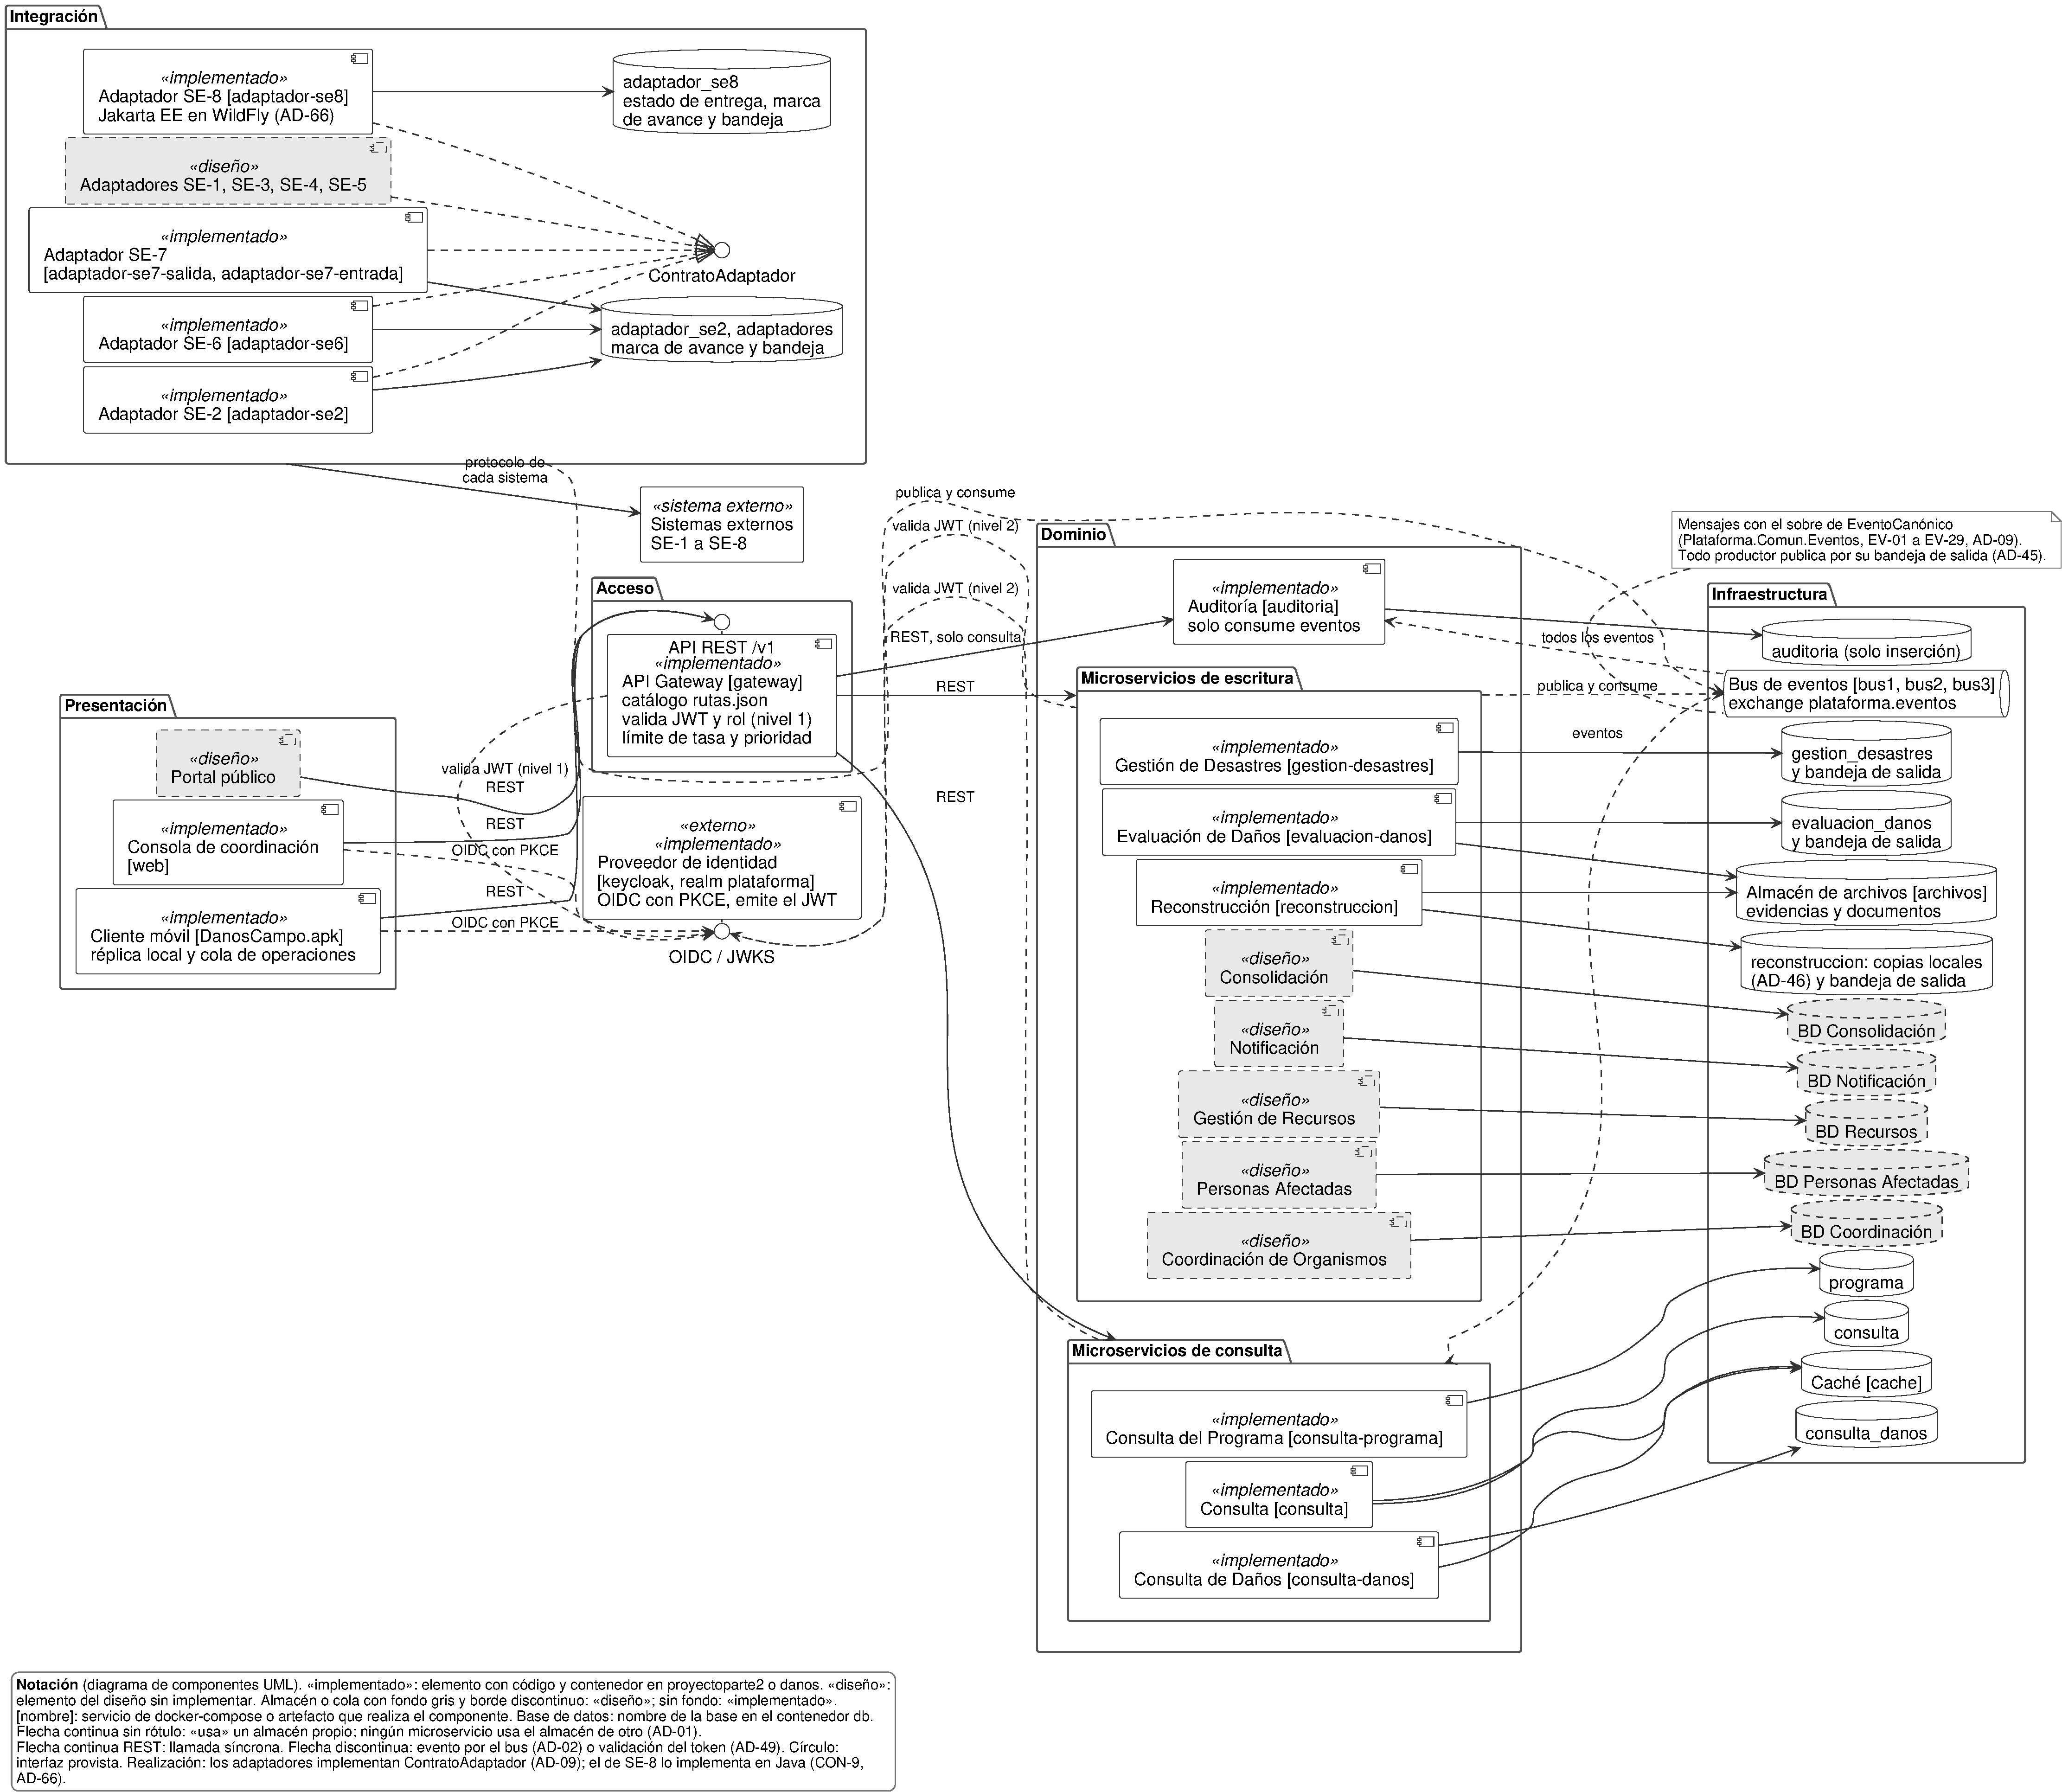
\includegraphics[width=\linewidth,height=0.86\textheight,keepaspectratio]{figuras/vista_logica}
\caption{Vista lógica (SAD 1.2). Diagrama de componentes UML por capas, con el alcance
implementado.}
\label{fig:vista-logica}
\end{figure}
\end{landscape}

\begin{landscape}
\begin{figure}[p]
\centering
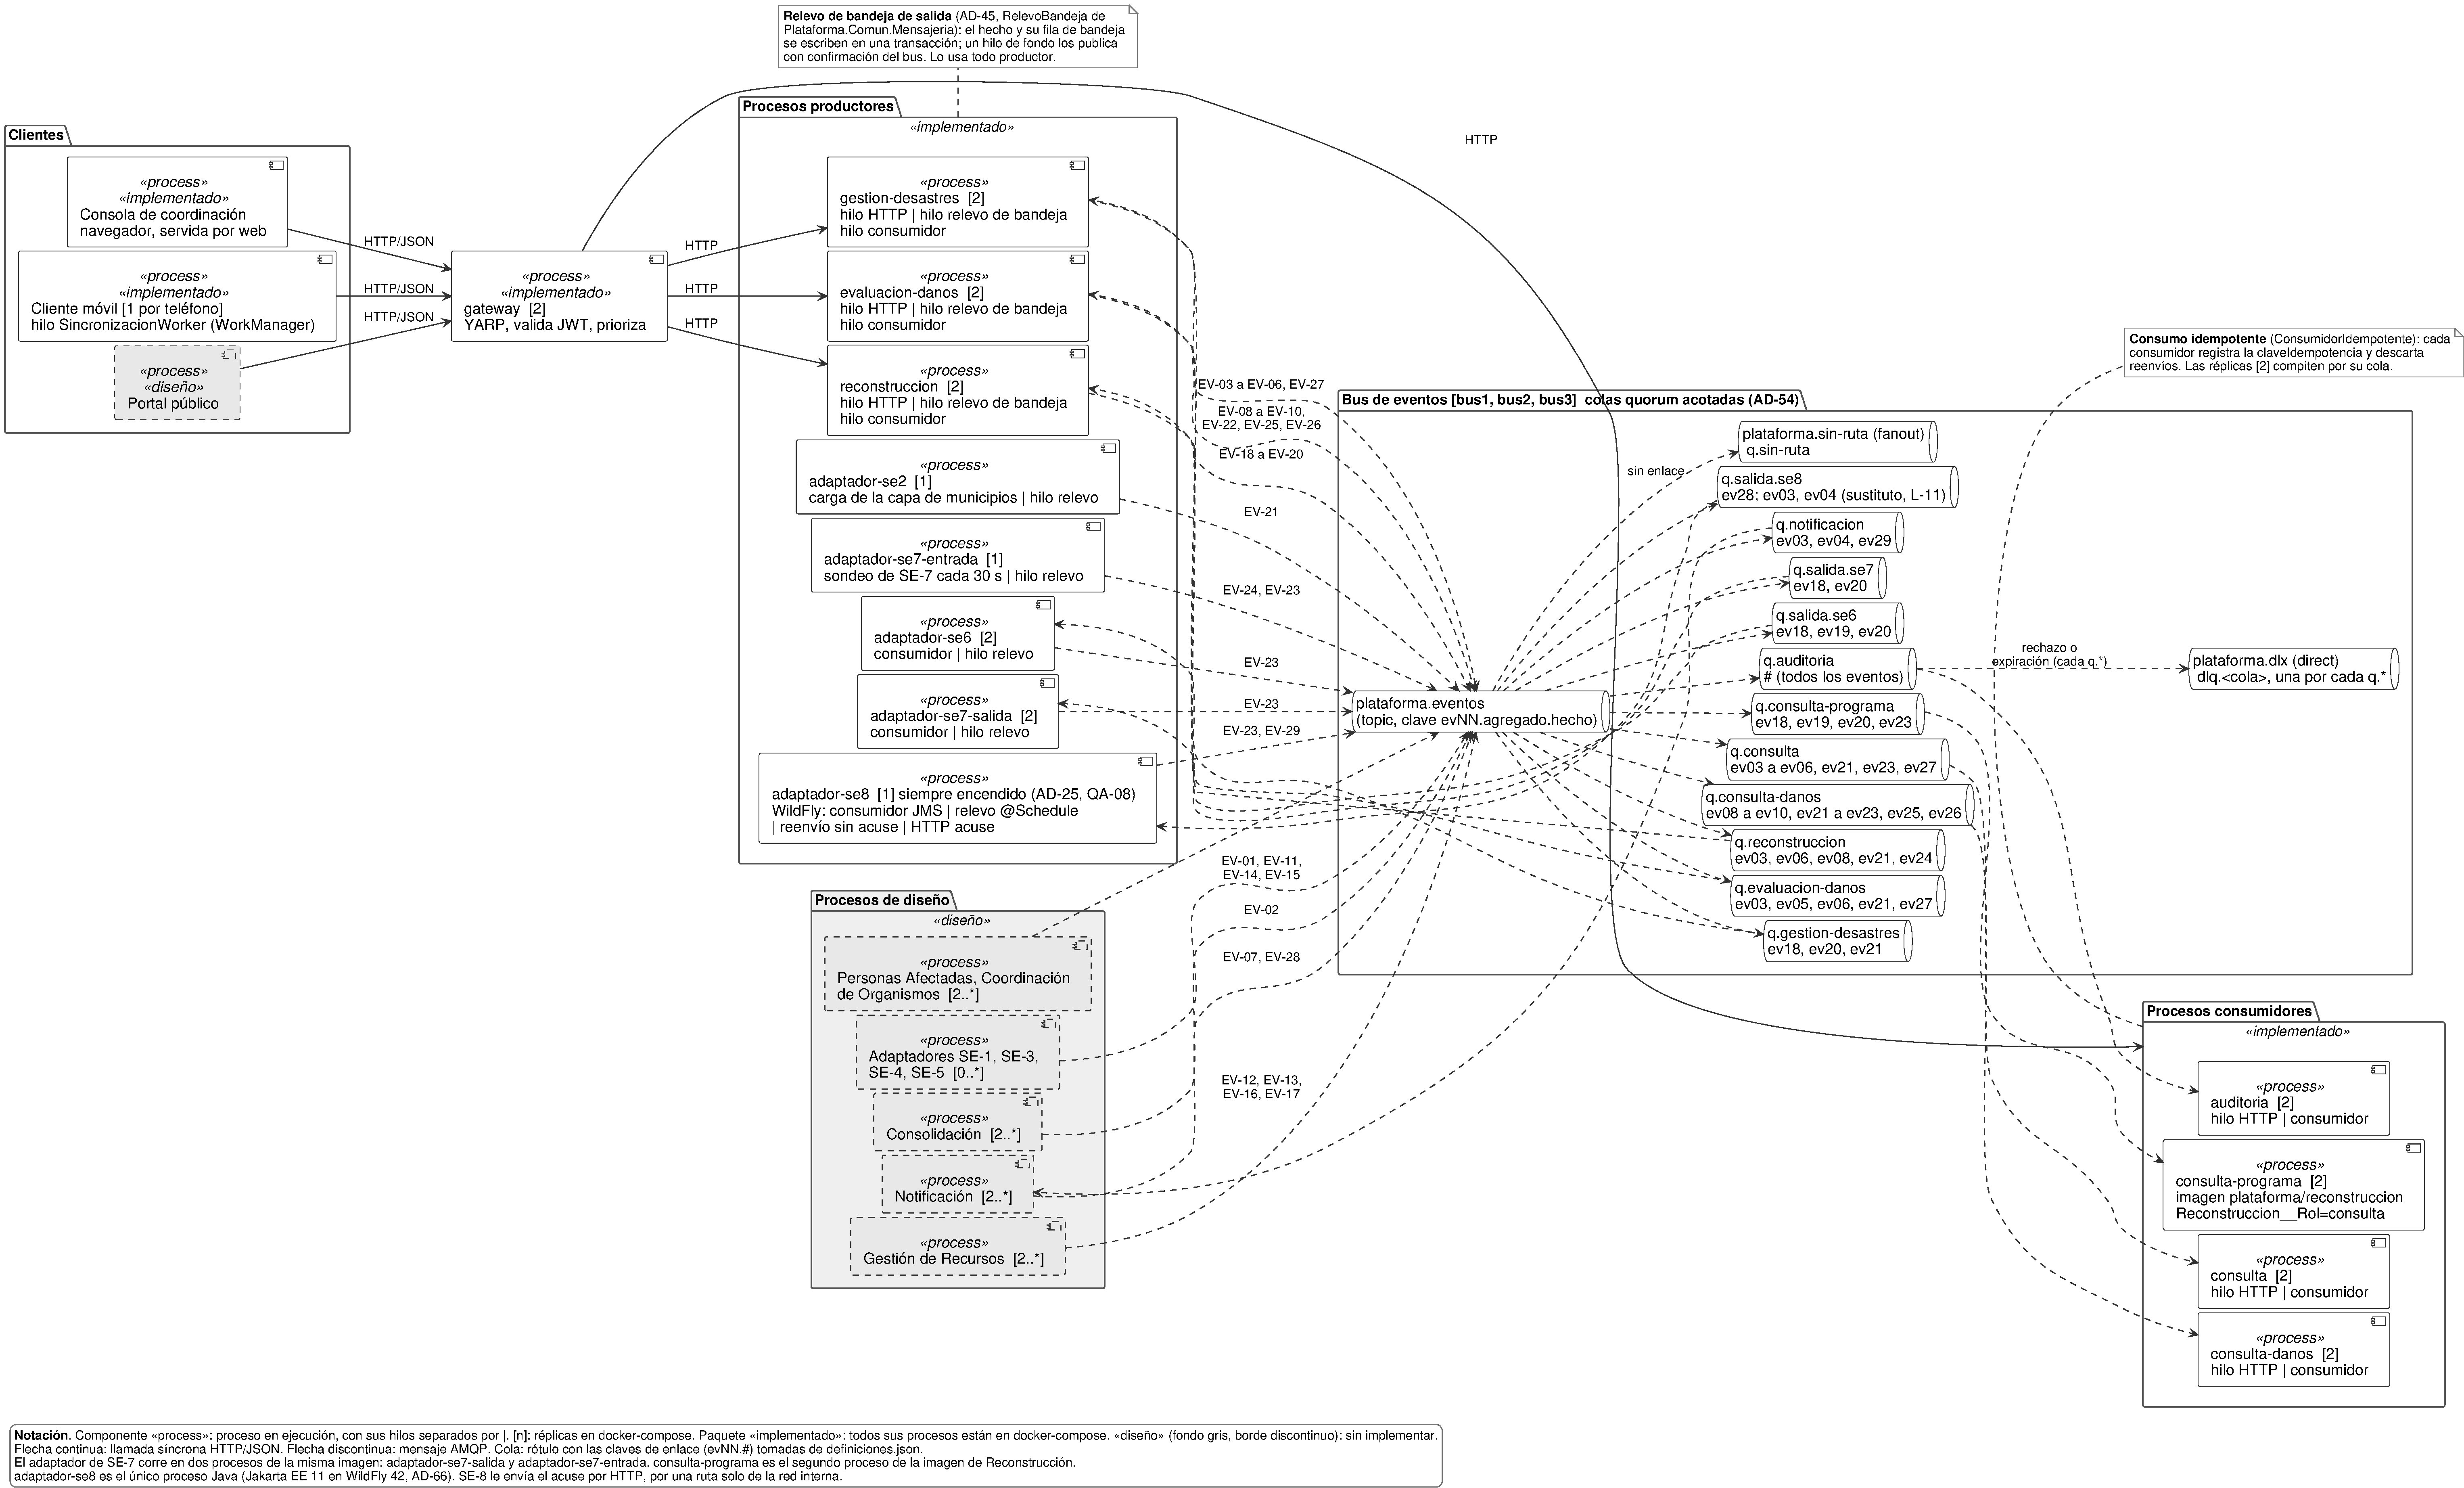
\includegraphics[width=\linewidth,height=0.86\textheight,keepaspectratio]{figuras/vista_procesos}
\caption{Vista de procesos (SAD 1.2). Procesos, réplicas, colas por consumidor y tácticas de
resiliencia.}
\label{fig:vista-procesos}
\end{figure}
\end{landscape}

\begin{landscape}
\begin{figure}[p]
\centering
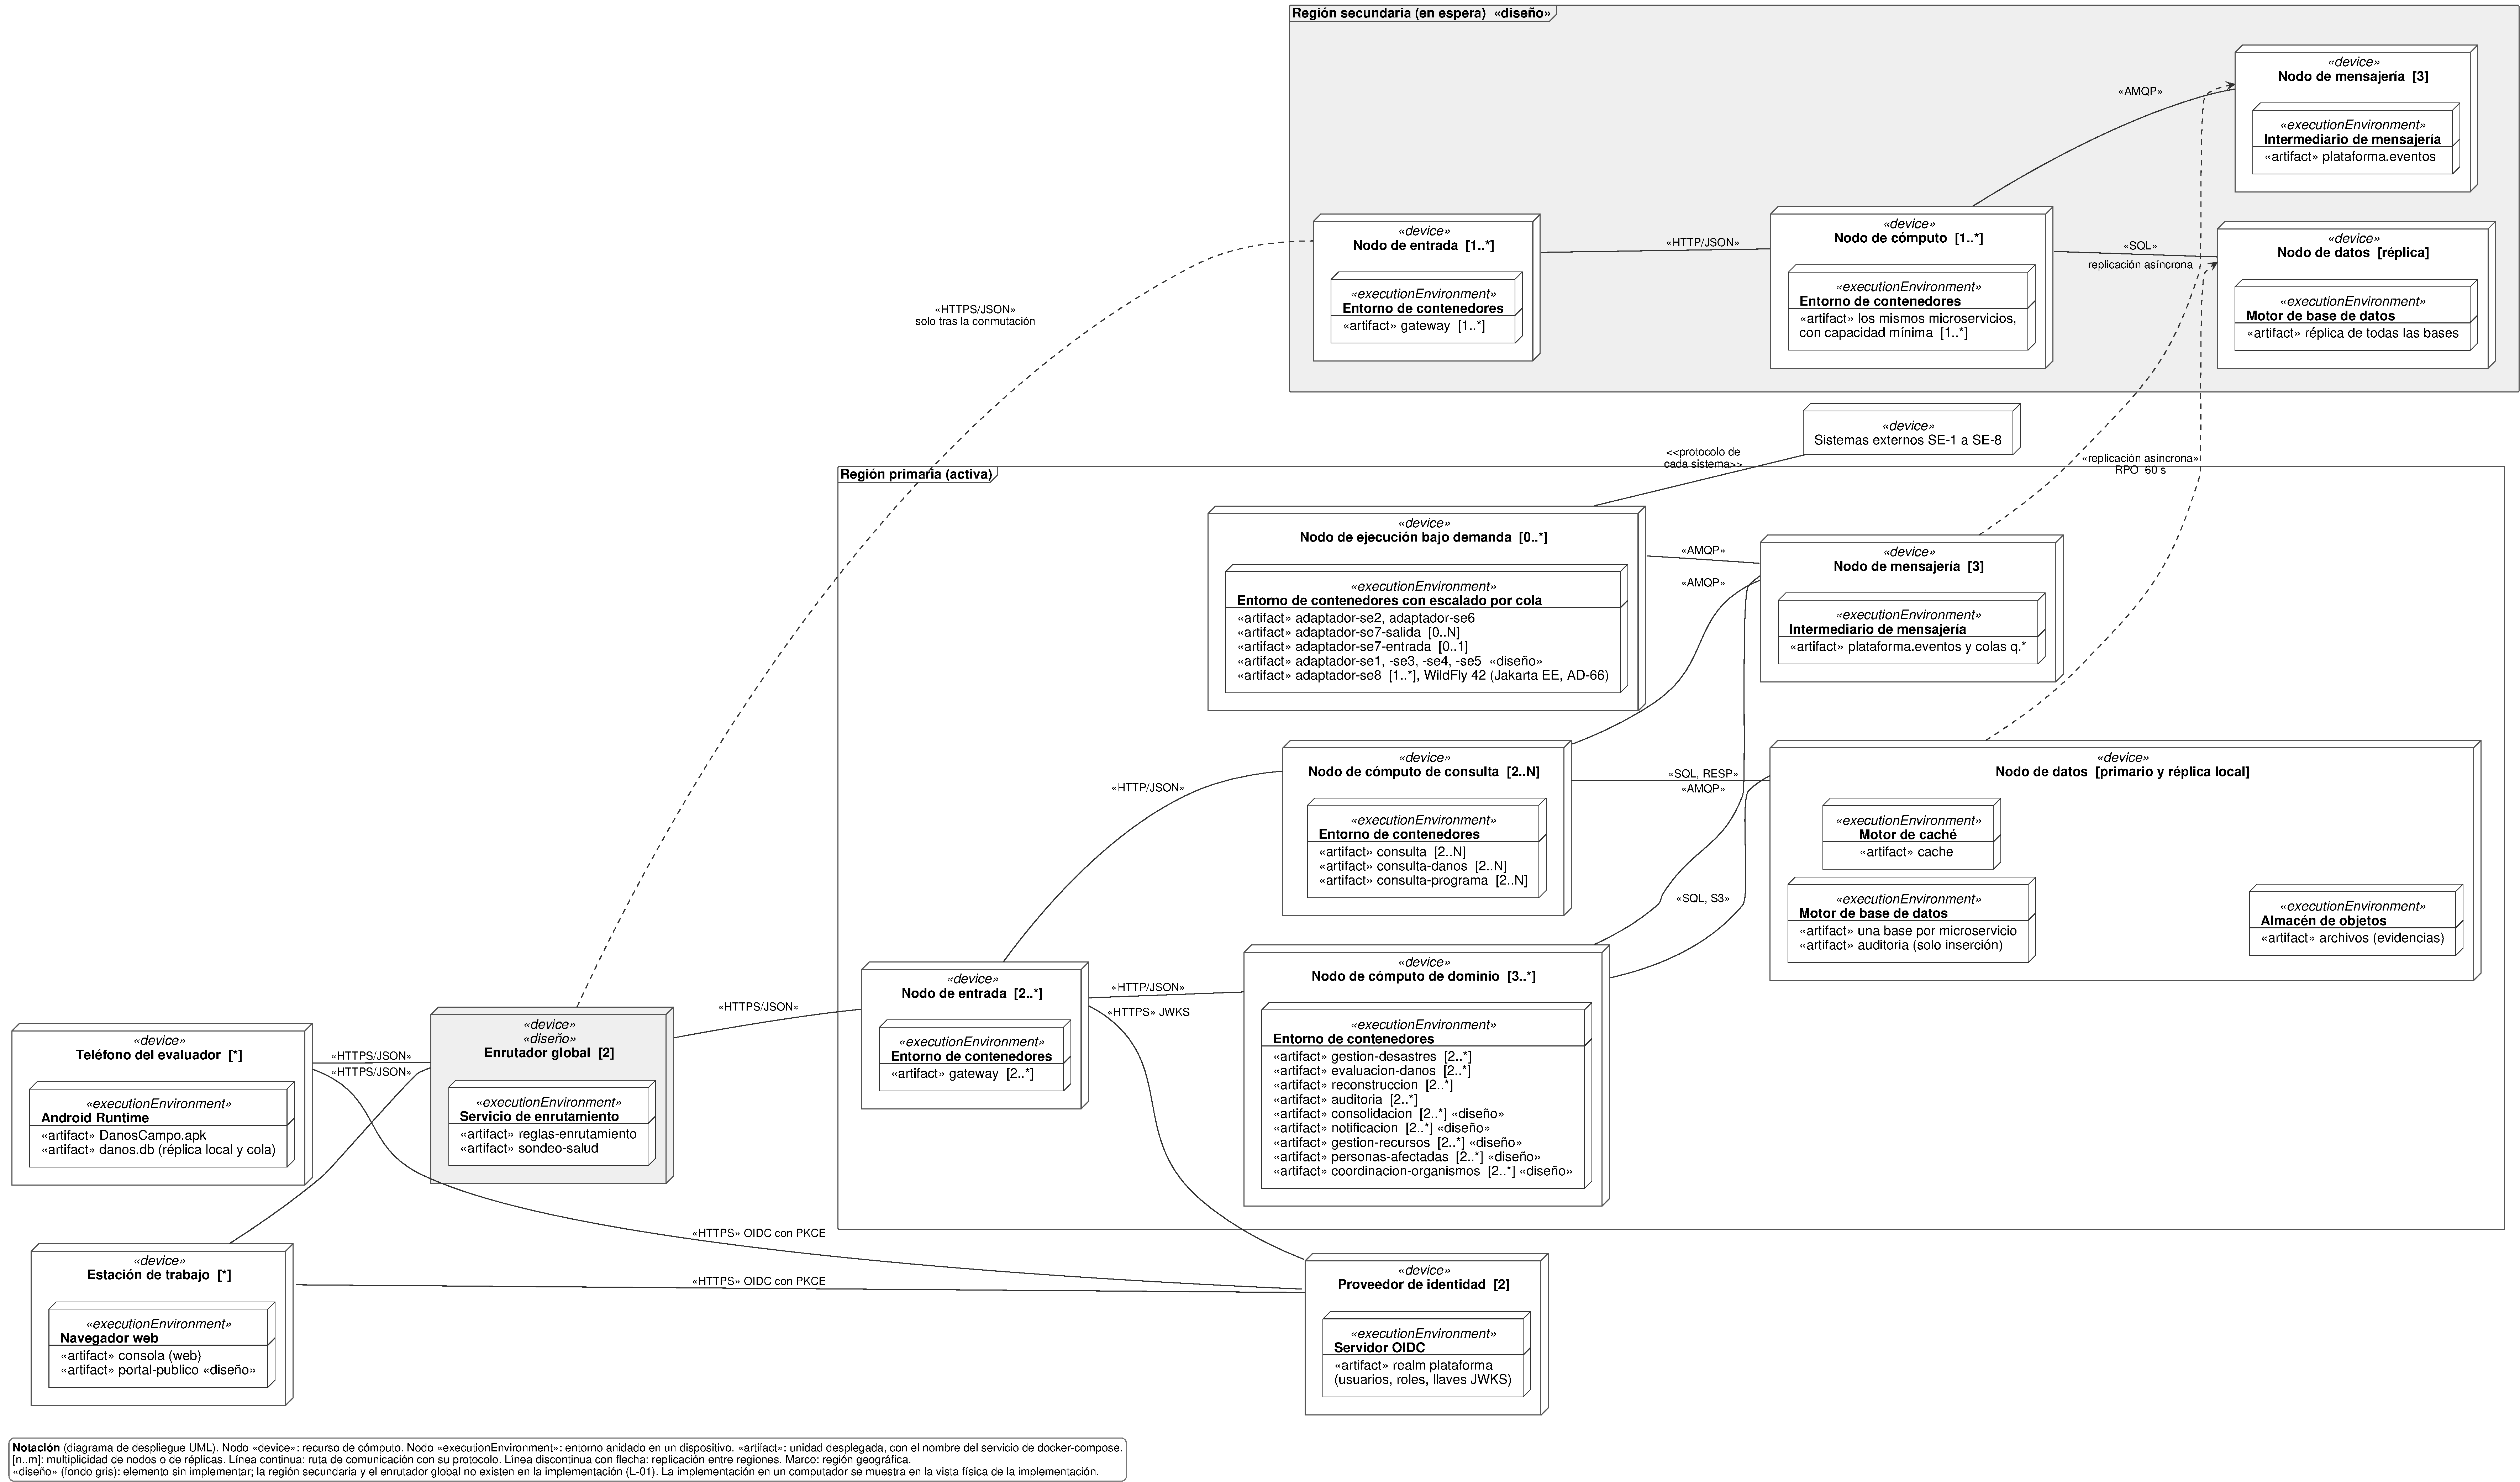
\includegraphics[width=\linewidth,height=0.86\textheight,keepaspectratio]{figuras/vista_despliegue}
\caption{Vista física del diseño (SAD 1.2). Diagrama de despliegue UML con dos regiones.}
\label{fig:vista-despliegue}
\end{figure}
\end{landscape}

\begin{landscape}
\begin{figure}[p]
\centering
\includegraphics[width=\linewidth,height=0.86\textheight,keepaspectratio]{figuras/vista_despliegue_implementacion}
\caption{Vista física de la implementación (SAD 1.2). Diagrama de despliegue UML de Docker Compose
y del teléfono Android.}
\label{fig:vista-despliegue-impl}
\end{figure}
\end{landscape}

%==============================================================================
\section{Paso 4. Identificación de los enfoques arquitectónicos}
\label{sec:paso4}

Los enfoques son los patrones y las tácticas que la arquitectura aplica \cite{bass}. Se identifican con
\texttt{EA-nn} y se relacionan con las decisiones del SAD que los materializan. Son la unidad de
análisis del paso 6: cada escenario se evalúa contra los enfoques que responden por él.

El \cref{tab:enfoques} indica, para cada enfoque, su categoría y el elemento en el que se ve. La
categoría dice si es un patrón, con el estilo al que pertenece, o una táctica, con su atributo y su
rama en Bass, Clements y Kazman \cite{bass}. La columna \enquote{Dónde se ve} remite a las vistas que
este documento reproduce (\cref{fig:vista-logica,fig:vista-procesos,fig:vista-despliegue,fig:vista-despliegue-impl})
y a sus secuencias (\cref{fig:seq-conmutacion,fig:seq-eo1,fig:seq-eo4,fig:seq-eo3}). Las demás figuras
se citan con su número en el SAD 1.2 \cite{sad}: Figura 5, vista de implementación; Figura 6, vista de
implementación del cliente móvil; Figura 11, registro del desastre en campo; y Figura 12, modelo de
integración. Cuando un mecanismo no está dibujado, la fila lo dice y remite a la decisión que lo
especifica.

La versión 1.1 agrega EA-19, que corresponde a la decisión AD-45, y amplía EA-16 con las decisiones
AD-43 y AD-44. La versión 1.2 amplía EA-19 a todo productor de eventos (E-19), agrega AD-46 y AD-47 a
EA-08 y agrega los enfoques EA-20 a EA-26, que resultan de la implementación.

\begin{longtable}{L{1.0cm} >{\RaggedRight\arraybackslash\hspace{0pt}}p{2.7cm} L{1.3cm} >{\RaggedRight\arraybackslash\hspace{0pt}}p{2.4cm} >{\RaggedRight\arraybackslash\hspace{0pt}}p{2.8cm} L{4.9cm}}
\cabecera{6}{tab:enfoques}{Enfoques arquitectónicos, categoría y elementos del diseño en los que se
ven}{\textbf{ID} & \textbf{Enfoque} & \textbf{Decisiones} & \textbf{Atributos} & \textbf{Categoría} &
\textbf{Dónde se ve}}
EA-01 & Microservicios con almacén propio, organizados en cuatro capas & AD-01, AD-08 &
Disponibilidad, escalabilidad, modificabilidad & Patrón microservicios (estilo basado en servicios) y
patrón capas (estilo llamada y retorno) & \cref{fig:vista-logica}: paquetes Presentación, Acceso,
Dominio e Infraestructura, y cada microservicio con su base. SAD, Figura 5: capas de
\texttt{evaluacion-danos} \\
EA-02 & Arquitectura dirigida por eventos, con bus intermediario y colas acotadas & AD-02 &
Disponibilidad, resiliencia, escalabilidad & Patrón publicación y suscripción (estilo basado en
eventos) & \cref{fig:vista-logica}: Bus de eventos. \cref{fig:vista-procesos}: exchange
\texttt{plataforma.eventos} y una cola \texttt{q.*} por consumidor. \cref{fig:vista-despliegue}: Nodo
de mensajería \\
EA-03 & Contrato de adaptador y evento canónico & AD-03, AD-09 & Interoperabilidad, modificabilidad &
Patrón adaptador. Táctica de integrabilidad, rama limitar dependencias: usar un intermediario &
\cref{fig:vista-logica}: paquete Integración, interfaz \texttt{ContratoAdaptador} y nota del bus sobre
\texttt{EventoCanónico}. SAD, Figuras 5 y 12: \texttt{IContratoAdaptador} \\
EA-04 & API Gateway como punto único de entrada, con límite de tasa y priorización & AD-04, AD-19 &
Seguridad, rendimiento, resiliencia & Patrón API Gateway (estilo basado en servicios). Táctica de
rendimiento, rama controlar la demanda: priorizar eventos & \cref{fig:vista-logica}: API Gateway.
\cref{fig:vista-procesos}: proceso \texttt{gateway} [2]. \cref{fig:vista-despliegue}: Nodo de entrada \\
EA-05 & Cortacircuitos por adaptador, con tiempo de espera y reintento & AD-05, AD-37 & Resiliencia,
disponibilidad & Táctica de disponibilidad. Detectar fallos: tiempo de espera. Prevenir fallos: retirar
de servicio. Recuperarse de fallos: reintento & \cref{fig:vista-procesos}: procesos
\texttt{adaptador-se6} y \texttt{adaptador-se7-salida}. SAD, Figura 12: componente Resiliencia.
Secuencia: \cref{fig:seq-eo3} \\
EA-06 & Marca de avance y consumo idempotente para recuperar el flujo de entrada & AD-14, AD-37 &
Disponibilidad, integridad & Táctica de disponibilidad, rama recuperarse de fallos: resincronización de
estado & \cref{fig:vista-logica}: base con la marca de avance de los adaptadores.
\cref{fig:vista-procesos}: nota de consumo idempotente. SAD, Figura 12: \texttt{MarcaAvance}.
Secuencia: \cref{fig:seq-eo3} \\
EA-07 & Catálogos de tipos y de categorías administrados en ejecución & AD-07, AD-28 & Modificabilidad
& Táctica de modificabilidad, rama diferir el enlace & \cref{fig:vista-logica}: componentes Gestión
de Desastres y Evaluación de Daños. Los catálogos son datos de sus bases y no se dibujan aparte \\
EA-08 & Modelo de lectura separado y copias locales, alimentados por eventos & AD-12, AD-15, AD-18,
AD-34, AD-42, AD-46, AD-47 & Escalabilidad, rendimiento & Patrón separación de lectura y escritura
(estilo basado en eventos) & \cref{fig:vista-logica}: paquete Microservicios de consulta, sus bases y
las copias locales de \texttt{reconstruccion}. \cref{fig:vista-procesos}: \texttt{consulta},
\texttt{consulta-danos} y \texttt{consulta-programa} con 2 réplicas, y colas \texttt{q.reconstruccion}
y \texttt{q.gestion-desastres}. \cref{fig:vista-despliegue}: multiplicidad de diseño [2..N] \\
EA-09 & Precálculo y caché de geometrías y de proyecciones & AD-17 & Rendimiento & Táctica de
rendimiento, rama gestionar recursos: mantener copias de los datos & \cref{fig:vista-logica}: almacén
Caché [\texttt{cache}] y bases de proyecciones. \cref{fig:vista-despliegue}: «artifact»
\texttt{cache}, en el Motor de caché \\
EA-10 & Historial versionado e historial de solo inserción & AD-20, AD-41 & Trazabilidad, integridad
& Táctica de seguridad, rama recuperarse de ataques: auditoría & \cref{fig:vista-logica}: bases
\texttt{gestion\_desastres}, \texttt{evaluacion\_danos} y \texttt{reconstruccion}. Las tablas de
historial están dentro de esas bases \\
EA-11 & Microservicio de Auditoría centralizado por eventos, con procedencia & AD-11, AD-21 &
Trazabilidad & Táctica de seguridad, rama recuperarse de ataques: auditoría & \cref{fig:vista-logica}:
Auditoría, base \texttt{auditoria} (solo inserción) y Consolidación. \cref{fig:vista-procesos}: cola
\texttt{q.auditoria} \\
EA-12 & Autorización en dos niveles y cifrado por columna & AD-22, AD-23 & Seguridad & Táctica de
seguridad, rama resistir ataques: autorizar actores y cifrar datos & \cref{fig:vista-logica}: API
Gateway (nivel 1), validación del JWT en los microservicios (nivel 2) y BD Personas Afectadas.
Secuencia: \cref{fig:seq-eo1} \\
EA-13 & Réplica activa local con sondeo de salud & AD-24 & Disponibilidad, resiliencia & Táctica de
disponibilidad. Detectar fallos: sondeo. Recuperarse de fallos: repuesto redundante &
\cref{fig:vista-procesos}: multiplicidades [2] y [2..*]. \cref{fig:vista-despliegue}: multiplicidad
[2..*] de los artefactos. \cref{fig:seq-conmutacion}: mensajes \enquote{sondeo de salud} \\
EA-14 & Despliegue en dos regiones, con réplica en espera, conmutación automática y resincronización &
AD-26, AD-27 & Recuperación ante fallos, disponibilidad & Táctica de disponibilidad, rama recuperarse
de fallos: repuesto redundante y resincronización de estado & \cref{fig:vista-despliegue}: regiones
primaria y secundaria, Enrutador global y «replicación asíncrona». Secuencia:
\cref{fig:seq-conmutacion} \\
EA-15 & Modelo híbrido de ejecución: microservicios persistentes y adaptadores efímeros & AD-25 &
Escalabilidad, rendimiento & Táctica de rendimiento, rama gestionar recursos: aumentar recursos &
\cref{fig:vista-procesos}: procesos persistentes y adaptadores [0..*]. \cref{fig:vista-despliegue}:
Nodo de ejecución bajo demanda \\
EA-16 & Réplica local sin conexión, con cola de operaciones y detección determinista de conflictos sin
resolución automática & AD-31, AD-32, AD-33, AD-43, AD-44 & Integridad de datos & Táctica de
disponibilidad, rama recuperarse de fallos: resincronización de estado & \cref{fig:vista-logica}:
Cliente móvil. \cref{fig:vista-despliegue}: Teléfono del evaluador con \texttt{danos.db}. SAD,
Figura 5: \texttt{ReglaConflicto}. Secuencia: \cref{fig:seq-eo4} \\
EA-17 & Reserva optimista con confirmación asíncrona y plazo de expiración & AD-38, AD-39 &
Disponibilidad, integridad & Táctica de disponibilidad, rama recuperarse de fallos: reversión al vencer
el plazo & \cref{fig:vista-logica}: Gestión de Recursos. \cref{fig:vista-procesos}: proceso Gestión de
Recursos [2..*]. El plazo de expiración no se dibuja: lo especifica AD-39 \\
EA-18 & Degradación controlada con marca de tiempo del dato & AD-16, AD-19 & Resiliencia,
disponibilidad & Táctica de disponibilidad, rama recuperarse de fallos: degradación &
\cref{fig:vista-procesos}: proceso \texttt{gateway}, que prioriza. \cref{fig:seq-eo3}: mensaje
\enquote{respuesta degradada y marcada} \\
EA-19 & Bandeja de salida transaccional en todo productor de eventos & AD-45, E-19 & Resiliencia,
integridad & Patrón bandeja de salida (estilo basado en eventos). Táctica de disponibilidad, rama
prevenir fallos: transacciones & \cref{fig:vista-logica}: bases con bandeja de salida y nota del bus.
\cref{fig:vista-procesos}: hilo relevo de bandeja y su nota. SAD, Figura 5: \texttt{RelevoBandeja}.
Secuencia: \cref{fig:seq-eo4} \\
EA-20 & Detección de huecos por secuencia del productor & AD-21, E-18, E-31 & Trazabilidad, integridad
& Táctica de seguridad, rama detectar ataques: anomalías en la entrega de mensajes &
\cref{fig:vista-procesos}: cola \texttt{q.auditoria}. SAD, Figura 5: \texttt{Sobre} y paquete
\texttt{Auditoria.*} \\
EA-21 & Cola acotada con rechazo de publicación, límite de entregas, cola de mensajes muertos y cola
sin ruta & AD-02, E-23, E-32 & Resiliencia, disponibilidad & Táctica de rendimiento, rama gestionar
recursos: acotar las colas. Táctica de disponibilidad, rama recuperarse de fallos: manejo de
excepciones & \cref{fig:vista-procesos}: colas \texttt{q.*}, \texttt{plataforma.dlx} con
\texttt{dlq.<cola>} y \texttt{plataforma.sin-ruta} con \texttt{q.sin-ruta}.
\cref{fig:vista-despliegue-impl}: \texttt{bus1}, \texttt{bus2} y \texttt{bus3} \\
EA-22 & Registro idempotente con identificador generado en el cliente & AD-44, AD-48, E-42 &
Integridad, disponibilidad & Táctica de disponibilidad, rama recuperarse de fallos: reintento & SAD,
Figura 6: paquetes del cliente móvil. SAD, Figura 11: registro con reenvío idempotente. Secuencia:
\cref{fig:seq-eo4} \\
EA-23 & Catálogo de rutas con regla de dominio, validado al arrancar & AD-04, AD-22 & Seguridad &
Táctica de seguridad, rama resistir ataques: limitar el acceso & \cref{fig:vista-logica}: API Gateway
con \texttt{rutas.json}. \cref{fig:vista-despliegue-impl}: \texttt{gateway} [2] y ruta con
\texttt{rutas.json} \\
EA-24 & Inicio de sesión OIDC con PKCE y token validado en el gateway y en cada servicio & AD-49, E-43
& Seguridad & Táctica de seguridad, rama resistir ataques: identificar y autenticar actores &
\cref{fig:vista-logica}: Proveedor de identidad. \cref{fig:vista-despliegue-impl}: \texttt{keycloak}.
SAD, Figura 5: \texttt{Plataforma.\br Comun.\br Seguridad} \\
EA-25 & Estado de integración publicado como EV-23 & AD-05, E-15 & Disponibilidad, interoperabilidad
& Táctica de disponibilidad, rama detectar fallos: monitor & SAD, Figura 12: \texttt{MonitorCircuito}
y \texttt{EstadoIntegracion}. \cref{fig:vista-procesos}: colas \texttt{q.consulta},
\texttt{q.consulta-danos} y \texttt{q.consulta-programa} \\
EA-26 & Umbrales y alarma de la bandeja de revisión & AD-32, E-13 & Integridad, operabilidad & Táctica
de disponibilidad, rama detectar fallos: monitoreo de condición & \cref{fig:vista-logica}: Consulta de
Daños y Evaluación de Daños. \cref{fig:vista-procesos}: cola \texttt{q.consulta-danos}. La bandeja se
ve en \cref{fig:seq-eo4} \\
\end{longtable}

%==============================================================================
\section{Paso 5. Generación del árbol de utilidad}
\label{sec:paso5}

El árbol de utilidad del SRS 1.2 se adopta sin cambios en la calificación de las hojas. La
priorización se hizo antes del diseño, y modificarla en la evaluación rompería la trazabilidad
entre ambos. Cada hoja tiene una calificación de importancia (I) y de dificultad (D), con la escala
Alta $= 3$, Media $= 2$ y Baja $= 1$, y una prioridad $P = I \times D$ \cite{srs}. La
\cref{fig:arbol} reproduce el árbol y el \cref{tab:arbol} lista sus quince hojas, ordenadas por
prioridad. Cada hoja enuncia el escenario con la medida única de su ficha en el SRS y la
característica de ISO/IEC 25010 \cite{iso25010} que le corresponde.

\begin{figure}[H]
\centering
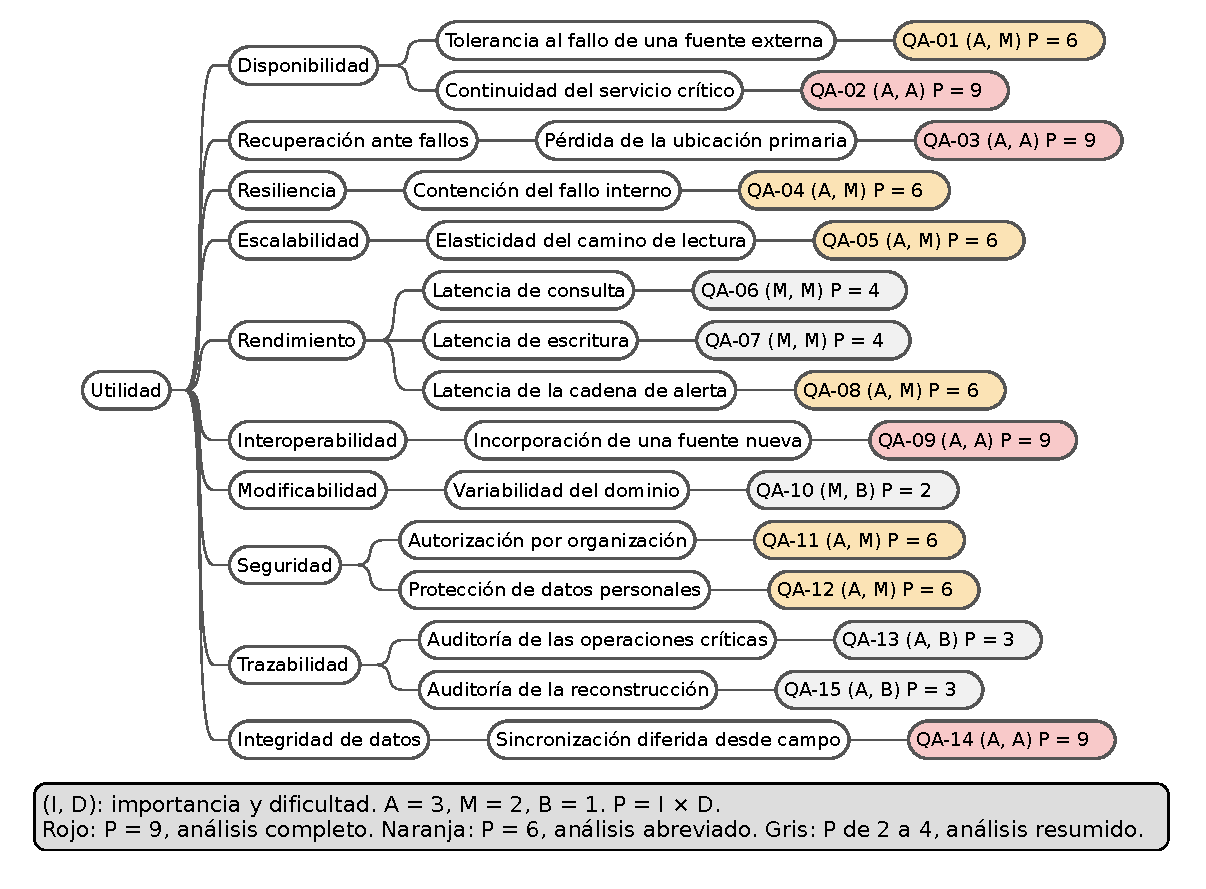
\includegraphics[width=\linewidth]{figuras/arbol_utilidad}
\caption{Árbol de utilidad con la calificación (importancia, dificultad) y la prioridad de cada
hoja.}
\label{fig:arbol}
\end{figure}

\begin{longtable}{L{1.1cm} >{\RaggedRight\arraybackslash\hspace{0pt}}p{2.1cm} L{4.9cm} >{\RaggedRight\arraybackslash\hspace{0pt}}p{2.8cm} C{1.1cm} C{0.5cm} L{1.8cm}}
\cabecera{7}{tab:arbol}{Hojas del árbol de utilidad, ordenadas por prioridad}{\textbf{ID} &
\textbf{Atributo} & \textbf{Escenario y medida única} & \textbf{Característica ISO/IEC 25010} &
\textbf{(I, D)} & \textbf{P} & \textbf{Análisis}}
QA-02 & Disponibilidad & Disponibilidad mensual de los servicios críticos $\ge$
\qty{99.95}{\percent} & Fiabilidad: disponibilidad & (A, A) & 9 & Completo \\
QA-03 & Recuperación ante fallos & Pérdida de la ubicación primaria: RTO $\le$ \qty{15}{\minute} con
RPO $\le$ \qty{60}{\second} & Fiabilidad: capacidad de recuperación & (A, A) & 9 & Completo \\
QA-09 & Interoperabilidad & Integrar un sistema externo nuevo con 0 componentes existentes modificados
& Compatibilidad: interoperabilidad & (A, A) & 9 & Completo \\
QA-14 & Integridad de datos & Sincronización de 120 evaluaciones con 5 conflictos: 0 evaluaciones
perdidas o sobrescritas en silencio & Seguridad: integridad & (A, A) & 9 & Completo \\
\midrule
QA-01 & Disponibilidad & Un sistema externo deja de responder: 0 funciones que no dependen de él
quedan indisponibles & Fiabilidad: tolerancia a fallos & (A, M) & 6 & Abreviado \\
QA-04 & Resiliencia & Un componente interno falla: 0 funciones críticas que no dependen de él quedan
indisponibles & Fiabilidad: tolerancia a fallos & (A, M) & 6 & Abreviado \\
QA-05 & Escalabilidad & De \num{1000} a \num{10000} usuarios concurrentes en \qty{10}{\minute}, con la
consulta frecuente en p95 $<$ \qty{2}{\second} & Eficiencia de desempeño: capacidad & (A, M) & 6 &
Abreviado \\
QA-08 & Rendimiento & Alerta crítica entregada con p95 $<$ \qty{5}{\second} & Eficiencia de desempeño:
comportamiento temporal & (A, M) & 6 & Abreviado \\
QA-11 & Seguridad & Un organismo no responsable intenta modificar un desastre ajeno:
\qty{100}{\percent} de rechazos sobre al menos 200 casos & Seguridad: integridad & (A, M) & 6 &
Abreviado \\
QA-12 & Seguridad & Lectura directa de los datos de personas afectadas: \qty{100}{\percent} de los
campos identificatorios ilegibles sin la clave & Seguridad: confidencialidad & (A, M) & 6 & Abreviado \\
\midrule
QA-06 & Rendimiento & Consulta frecuente con p95 $<$ \qty{2}{\second} bajo \num{10000} usuarios &
Eficiencia de desempeño: comportamiento temporal & (M, M) & 4 & Resumido \\
QA-07 & Rendimiento & Registro de un evento con p95 $<$ \qty{3}{\second} & Eficiencia de desempeño:
comportamiento temporal & (M, M) & 4 & Resumido \\
QA-13 & Trazabilidad & Rastro de las cinco clases de operación crítica: \qty{100}{\percent} de las
operaciones con entrada de auditoría & Seguridad: responsabilidad y no repudio & (A, B) & 3 & Resumido \\
QA-15 & Trazabilidad & Cambios de presupuesto y de estado de un proyecto: \qty{100}{\percent} con
entrada de valor anterior y valor nuevo & Seguridad: responsabilidad y no repudio & (A, B) & 3 &
Resumido \\
QA-10 & Modificabilidad & Incorporar un tipo de desastre con 0 componentes modificados o redesplegados
& Mantenibilidad: capacidad de ser modificado & (M, B) & 2 & Resumido \\
\end{longtable}

Las quince hojas provienen de requisitos documentados en el SRS. El árbol no incluye escenarios de
crecimiento ni exploratorios. Esos escenarios se generan en el paso 7.

Dos clasificaciones merecen una justificación. La recuperación (QA-03) pertenece a la categoría de
disponibilidad de Bass, Clements y Kazman \cite{bass}, y se trata en una hoja aparte por tres razones:
el enunciado la nombra como atributo propio \cite{enunciado}, ISO/IEC 25010 distingue la disponibilidad
de la capacidad de recuperación \cite{iso25010}, y su estímulo y su medida son otros. QA-02 mide la
proporción de tiempo de servicio en un mes, ante fallos que las réplicas absorben. QA-03 mide cuánto
tarda el servicio en volver y cuántos datos se pierden cuando se pierde una ubicación completa. El
compromiso T-08 muestra que ambas medidas se relacionan, y por eso se analizan juntas.

QA-09 se clasifica como interoperabilidad y no como extensibilidad. La pregunta es válida, porque la
plataforma se amplía con un adaptador sin modificar lo existente. Sin embargo, el estímulo del
escenario es intercambiar información con un sistema externo heterogéneo, y su resultado es que ese
intercambio funciona, sin que la plataforma gane una función de dominio nueva. Eso corresponde a
Compatibilidad: interoperabilidad en ISO/IEC 25010. La medida usa el vocabulario de la integrabilidad
\cite{bass}: componentes modificados. La extensibilidad del dominio se evalúa en QA-10, donde lo que
se agrega es un tipo de desastre.

El análisis se asigna según la prioridad:

\begin{itemize}
  \item Las cuatro hojas con $P = 9$ concentran el riesgo arquitectónico y reciben un análisis
        completo en el paso 6 (\cref{sec:qa02,sec:qa03,sec:qa09,sec:qa14}).
  \item Las seis hojas con $P = 6$ reciben un análisis abreviado, con los mismos campos
        (\cref{sec:abreviado}).
  \item Las cinco hojas con $P \le 4$ reciben un análisis resumido (\cref{sec:resumido}). Los
        mecanismos que las resuelven son conocidos y su riesgo técnico es bajo. QA-13 y QA-15
        tienen importancia Alta y dificultad Baja.
\end{itemize}

%==============================================================================
\newpage
\section{Paso 6. Análisis de los enfoques arquitectónicos}
\label{sec:paso6}

Cada ficha analiza un escenario contra los enfoques que responden por él. El razonamiento compara
la opción elegida con las alternativas descartadas en la iteración de ADD correspondiente
\cite{iteraciones}. Cada ficha indica los componentes impactados, los puntos de sensibilidad
(\cref{tab:sensibilidad}), los compromisos (\cref{tab:tradeoffs}), los riesgos (\cref{tab:riesgos})
y los no riesgos. Los diagramas de secuencia muestran el comportamiento que se analiza.

\subsection{QA-02: Disponibilidad de los servicios críticos}
\label{sec:qa02}

\begin{longtable}{L{3.0cm} L{12.8cm}}
\cabecera{2}{tab:f-qa02}{Análisis de QA-02}{\textbf{Campo} & \textbf{Análisis}}
Escenario & Disponibilidad mensual $\ge$ \qty{99.95}{\percent} ($\le$ \qty{21.6}{\minute} al mes) de
los servicios críticos. Calificación (A, A), $P = 9$ \\
Enfoques & EA-01, microservicios con fallo aislado. EA-02, bus que desacopla productor y consumidor.
EA-13, réplicas activas con sondeo. EA-14, dos regiones con conmutación automática. EA-18,
degradación controlada \\
Componentes impactados & API Gateway y los microservicios que prestan los servicios críticos:
Gestión de Desastres, Consulta, Notificación y Coordinación de Organismos. Bus de eventos y
enrutador global (\cref{fig:vista-procesos,fig:vista-despliegue}) \\
Razonamiento & Se descartaron dos alternativas. El reinicio manual depende de que una persona
detecte el fallo, lo que no puede garantizarse durante una emergencia. La reposición automática sin
réplica activa detecta y repone la instancia, pero deja un intervalo sin servicio mientras la
instancia arranca. Con réplicas activas (EA-13), las demás réplicas ya atienden tráfico cuando una
falla, y el sondeo de salud retira la réplica fallida en \qty{30}{\second} o menos, que es el plazo
que fija la respuesta de QA-02 en el SRS. La primera parte de la \cref{fig:seq-conmutacion} muestra este comportamiento.\newline
El fallo de un componente interno completo se atiende con el mismo mecanismo y con el bus de eventos
(EA-02), que retiene los mensajes y los entrega cuando el componente se recupera. La degradación
controlada (EA-18) protege los servicios críticos ante un exceso de carga: se reduce primero el
portal público. La conmutación regional (QA-03) es el evento que más consume del margen mensual:
hasta \qty{15}{\minute} en una sola ocurrencia \\
Sensibilidad & PS-01, número de réplicas activas por microservicio. Con una réplica no hay
redundancia. Con dos se tolera un fallo simultáneo y con tres se toleran dos. La conmutación
regional no depende de este número, porque se pierde la región completa. Su efecto se analiza en
QA-03 (PS-13) \\
Compromiso & Mantener réplicas activas tiene un costo de operación, que no afecta a otro driver.
T-12: validar el token en cada servicio hace que todos dependan del proveedor de identidad \\
Riesgos & R-04. Una conmutación regional consume cerca de \qty{15}{\minute} de los
\qty{21.6}{\minute} mensuales y deja \qty{6.6}{\minute} para cualquier otro fallo del mes. Se
registra como el compromiso T-08. R-13: un cambio de llaves del proveedor de identidad hace que los
servicios rechacen tokens válidos hasta reiniciarse \\
No riesgos & Un fallo de instancia no produce indisponibilidad perceptible, mientras haya al menos
dos réplicas activas por servicio crítico y el sondeo retire la réplica fallida en \qty{30}{\second}
o menos \\
\end{longtable}

\subsection{QA-03: Recuperación ante la pérdida de la ubicación primaria}
\label{sec:qa03}

\begin{longtable}{L{3.0cm} L{12.8cm}}
\cabecera{2}{tab:f-qa03}{Análisis de QA-03}{\textbf{Campo} & \textbf{Análisis}}
Escenario & Conmutación con RTO $\le$ \qty{15}{\minute} y RPO $\le$ \qty{60}{\second}. Calificación
(A, A), $P = 9$ \\
Enfoques & EA-14, réplica en espera en una segunda región, conmutación automática y
resincronización de estado. EA-02, bus como punto de retención de los eventos en tránsito \\
Componentes impactados & Enrutador global, todos los nodos de la región primaria y de la región
secundaria, y la replicación entre los nodos de datos y entre los nodos de mensajería
(\cref{fig:vista-despliegue}) \\
Razonamiento & Se descartaron dos alternativas. Un solo centro de cómputo no resiste el escenario
del dominio, en el que el desastre puede inutilizarlo. Varias sedes en la misma ciudad protegen ante
un fallo local y no ante un sismo regional.\newline
La región secundaria tiene los microservicios desplegados y recibe los datos por replicación
continua. Por eso la conmutación consiste en activar la región y aumentar su capacidad, lo que es
compatible con un RTO de \qty{15}{\minute}. El RPO de \qty{60}{\second} resulta de la replicación
asíncrona: en el instante del fallo hay datos que solo existen en la primaria. Cuando la primaria se
recupera, la resincronización (AD-27) hace converger sus datos con los de la región activa. La
segunda parte de la \cref{fig:seq-conmutacion} muestra la conmutación y la recuperación \\
Sensibilidad & PS-02, retardo de la replicación asíncrona entre regiones. Si su p99 pasa del umbral
de alarma (\qty{30}{\second}) hacia el límite de \qty{60}{\second}, el RPO real incumple la
medida. PS-13, valor del RTO \\
Compromiso & T-02 (AD-26). La replicación es asíncrona para no aumentar la latencia de escritura
(QA-07), y eso fija el RPO en hasta \qty{60}{\second}. Con replicación síncrona, el RPO sería
cercano a cero, pero cada escritura esperaría el acuse de la región secundaria. El compromiso se
resuelve a favor de la latencia de escritura \\
Riesgos & R-09. El SAD no especifica qué ocurre con un evento publicado en la primaria que no se
había replicado al bus de la secundaria en el instante del fallo. Esto puede afectar los 0 eventos
perdidos que exige la respuesta de QA-04 \\
No riesgos & La región secundaria recibe tráfico dentro del RTO, mientras la conmutación sea
automática y no dependa de un operador \\
\end{longtable}

\begin{figure}[p]
\centering
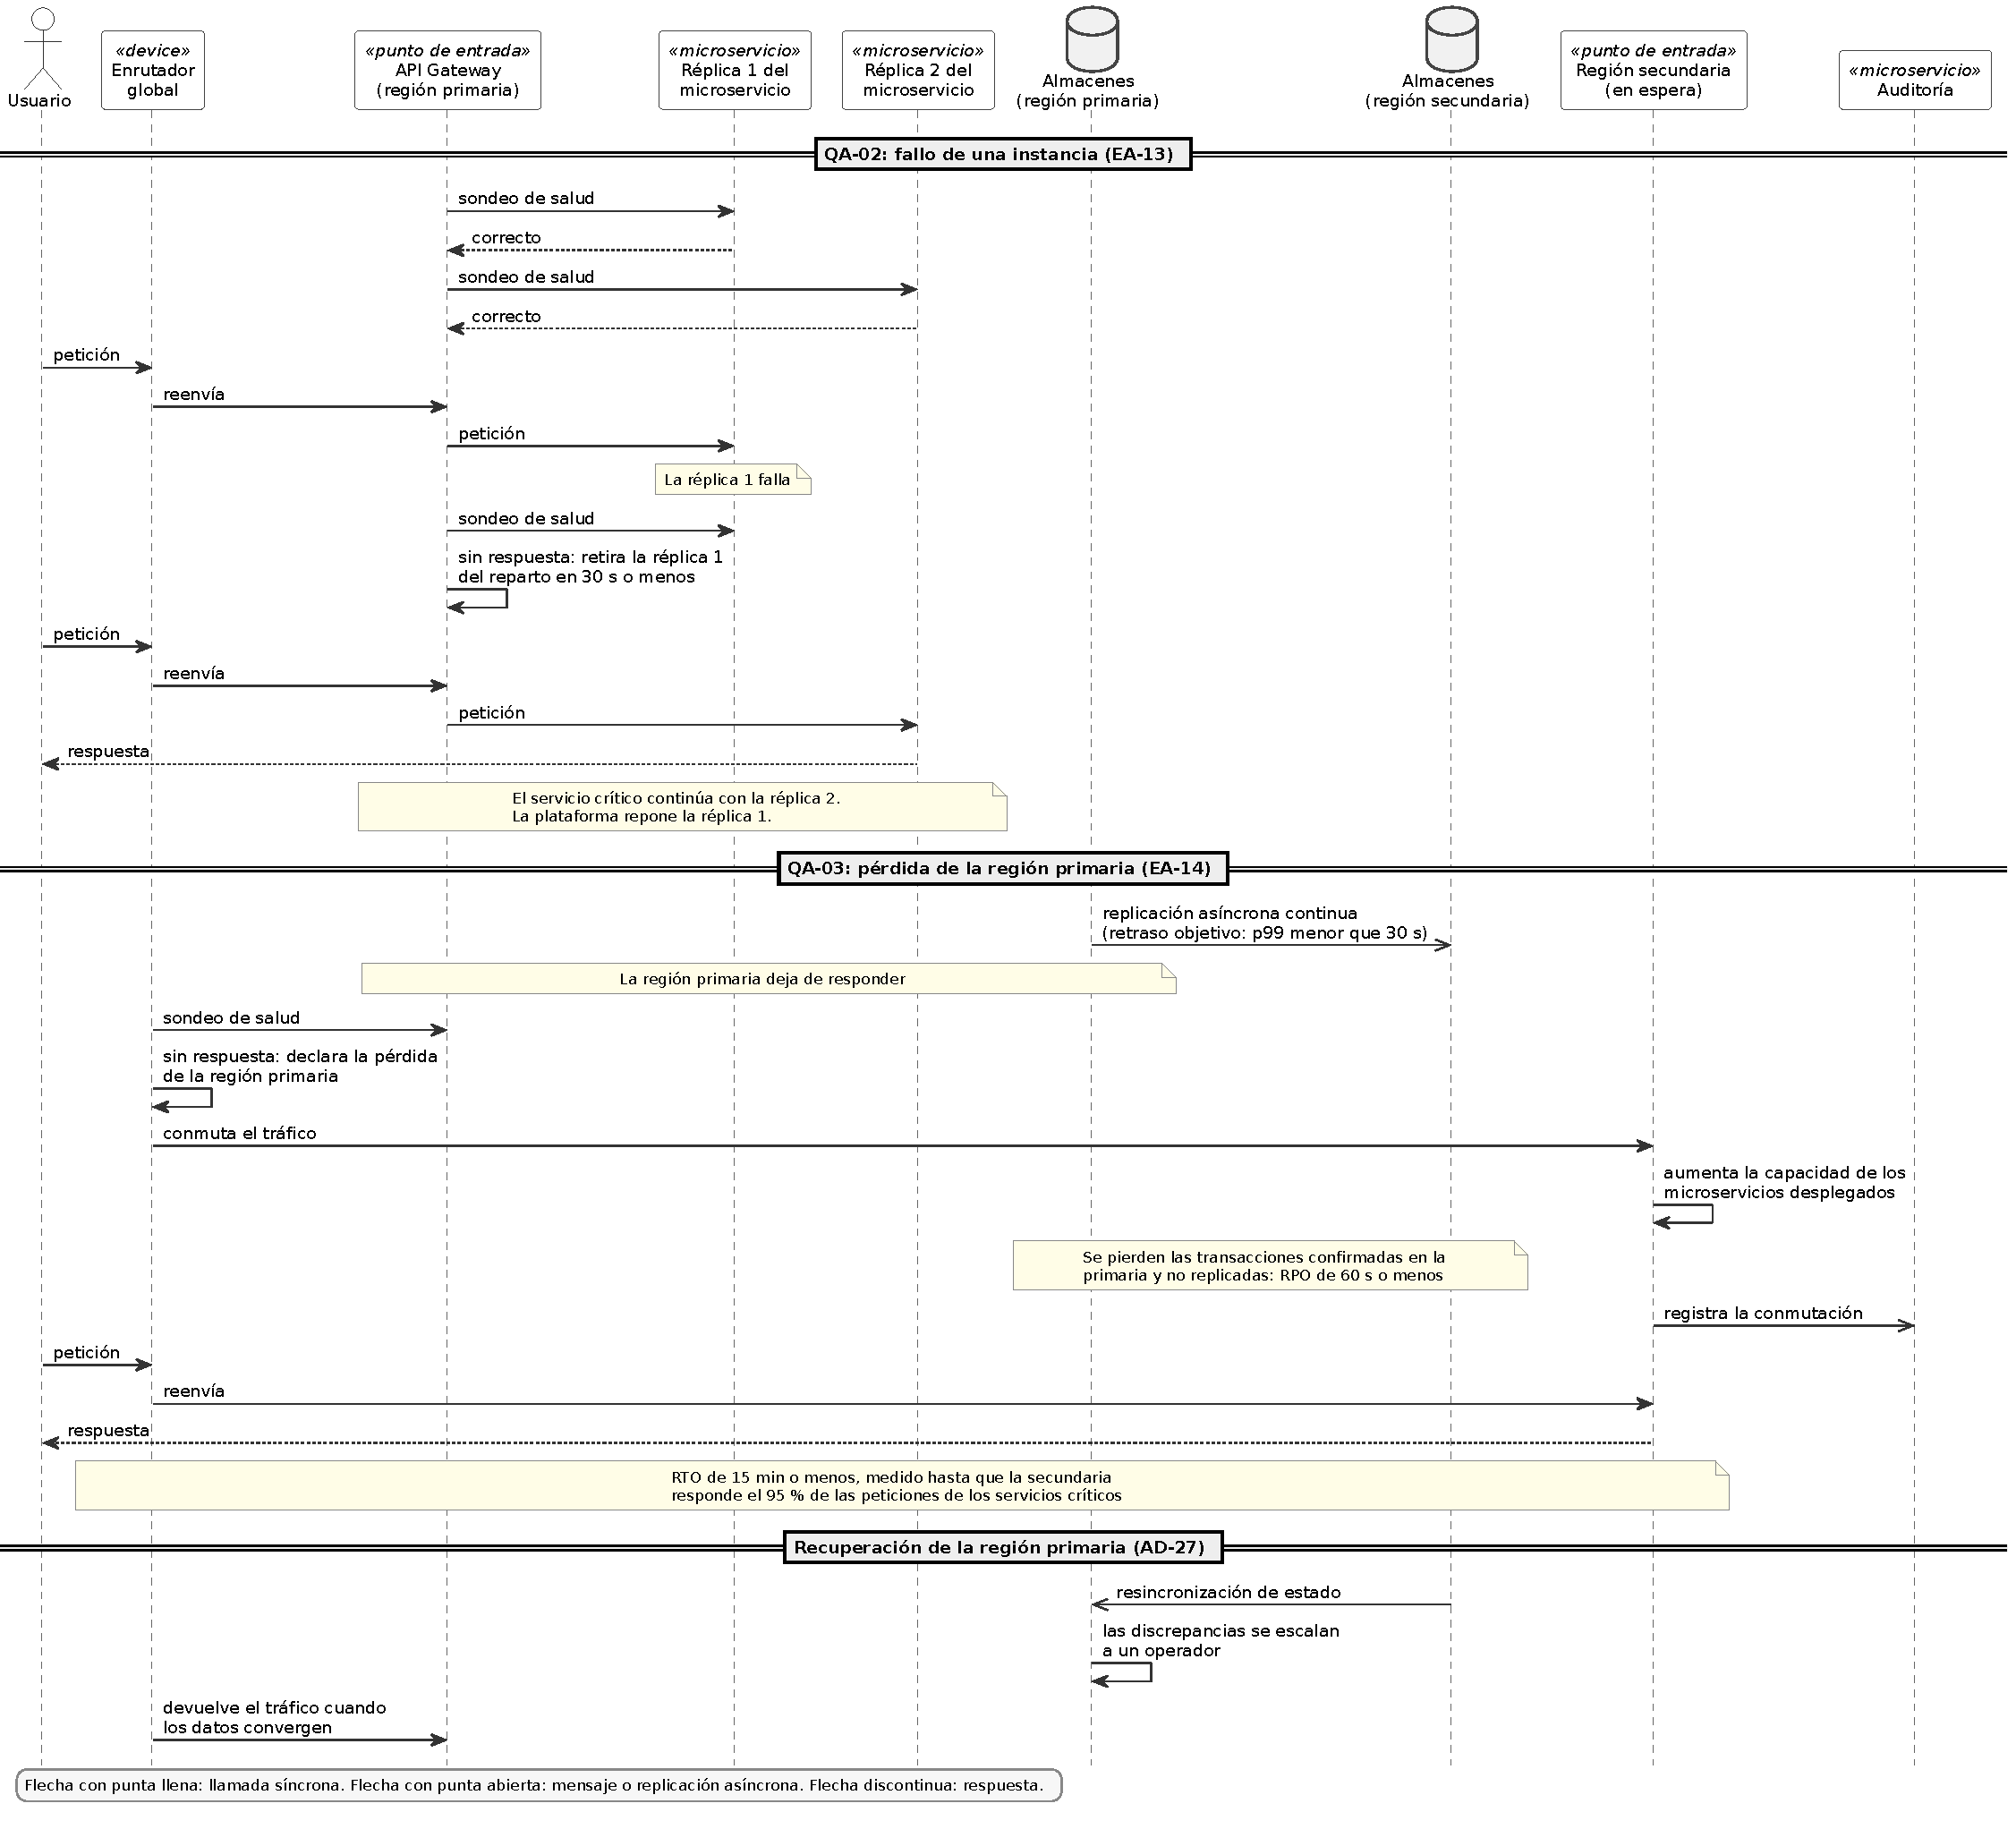
\includegraphics[width=\linewidth,height=0.9\textheight,keepaspectratio]{figuras/seq_conmutacion}
\caption{Diagrama de secuencia de QA-02 y QA-03: fallo de una instancia, pérdida de la región
primaria y recuperación.}
\label{fig:seq-conmutacion}
\end{figure}
\clearpage

\subsection{QA-09: Incorporación de un sistema externo nuevo}
\label{sec:qa09}

\begin{longtable}{L{3.0cm} L{12.8cm}}
\cabecera{2}{tab:f-qa09}{Análisis de QA-09}{\textbf{Campo} & \textbf{Análisis}}
Escenario & Integrar un sistema externo nuevo con 0 componentes existentes modificados. Calificación
(A, A), $P = 9$ \\
Enfoques & EA-03, contrato de adaptador y evento canónico. EA-05, cortacircuitos propio. EA-06,
marca de avance. EA-15, adaptadores como unidades efímeras \\
Componentes impactados & Se agrega un adaptador y su cola de salida en el bus. No cambian los doce
microservicios, el paquete común ni los ocho adaptadores existentes (SAD, cuadro \enquote{Qué se
modifica para...}) \\
Razonamiento & Se descartaron dos alternativas en la iteración 3. Una interfaz propia por adaptador
obligaría a los microservicios de dominio a conocer cada forma de recibir información, y agregar un
sistema los modificaría. Un adaptador genérico configurable no cubre la heterogeneidad de protocolo,
formato y frecuencia de los sistemas, y cada sistema nuevo modificaría ese componente
compartido.\newline
Con el contrato de adaptador y el evento canónico (EA-03), los microservicios conocen el evento
canónico y no los sistemas externos. Incorporar un sistema consiste en escribir un adaptador que
implementa el contrato. El modelo de integración del SAD aplica el contrato a ocho sistemas
distintos (alertas, GIS, hospitalario, recursos, personas afectadas, financiero, proyectos y
notificación). La \cref{fig:seq-eo1} muestra el recorrido de un dato de SE-1: el adaptador publica
EV-01 y ningún microservicio invoca a SE-1.\newline
El esfuerzo de 15 días-persona que fija la respuesta del escenario se limita a lo específico del
sistema nuevo. El contrato, el esquema
del evento, el cortacircuitos (EA-05) y la marca de avance (EA-06) se reutilizan. El adaptador se
despliega como unidad efímera (EA-15), sin capacidad reservada \\
Sensibilidad & PS-03, expresividad del contrato de adaptador y del esquema del evento canónico. Un
contrato más estrecho reduce el costo de cada adaptador y excluye sistemas cuyo dato no cabe en el
esquema. Un contrato más amplio admite más sistemas, traslada complejidad a cada adaptador y
permite que los microservicios dependan de campos que no todo evento contiene \\
Compromiso & T-09 (AD-09). Se favorece la interoperabilidad frente a la modificabilidad del
contrato: ocho adaptadores dependen de él, y un cambio del contrato los afecta a todos \\
Riesgos & R-03. La cifra de 15 días-persona supone que el sistema nuevo se expresa con el esquema
vigente del evento canónico. Un sistema cuyo dato no se ajuste obligaría a extender el contrato
compartido \\
No riesgos & Agregar un sistema externo no modifica ningún microservicio de dominio, mientras el
sistema nuevo se exprese por completo con el evento canónico vigente \\
\end{longtable}

\begin{landscape}
\begin{figure}[p]
\centering
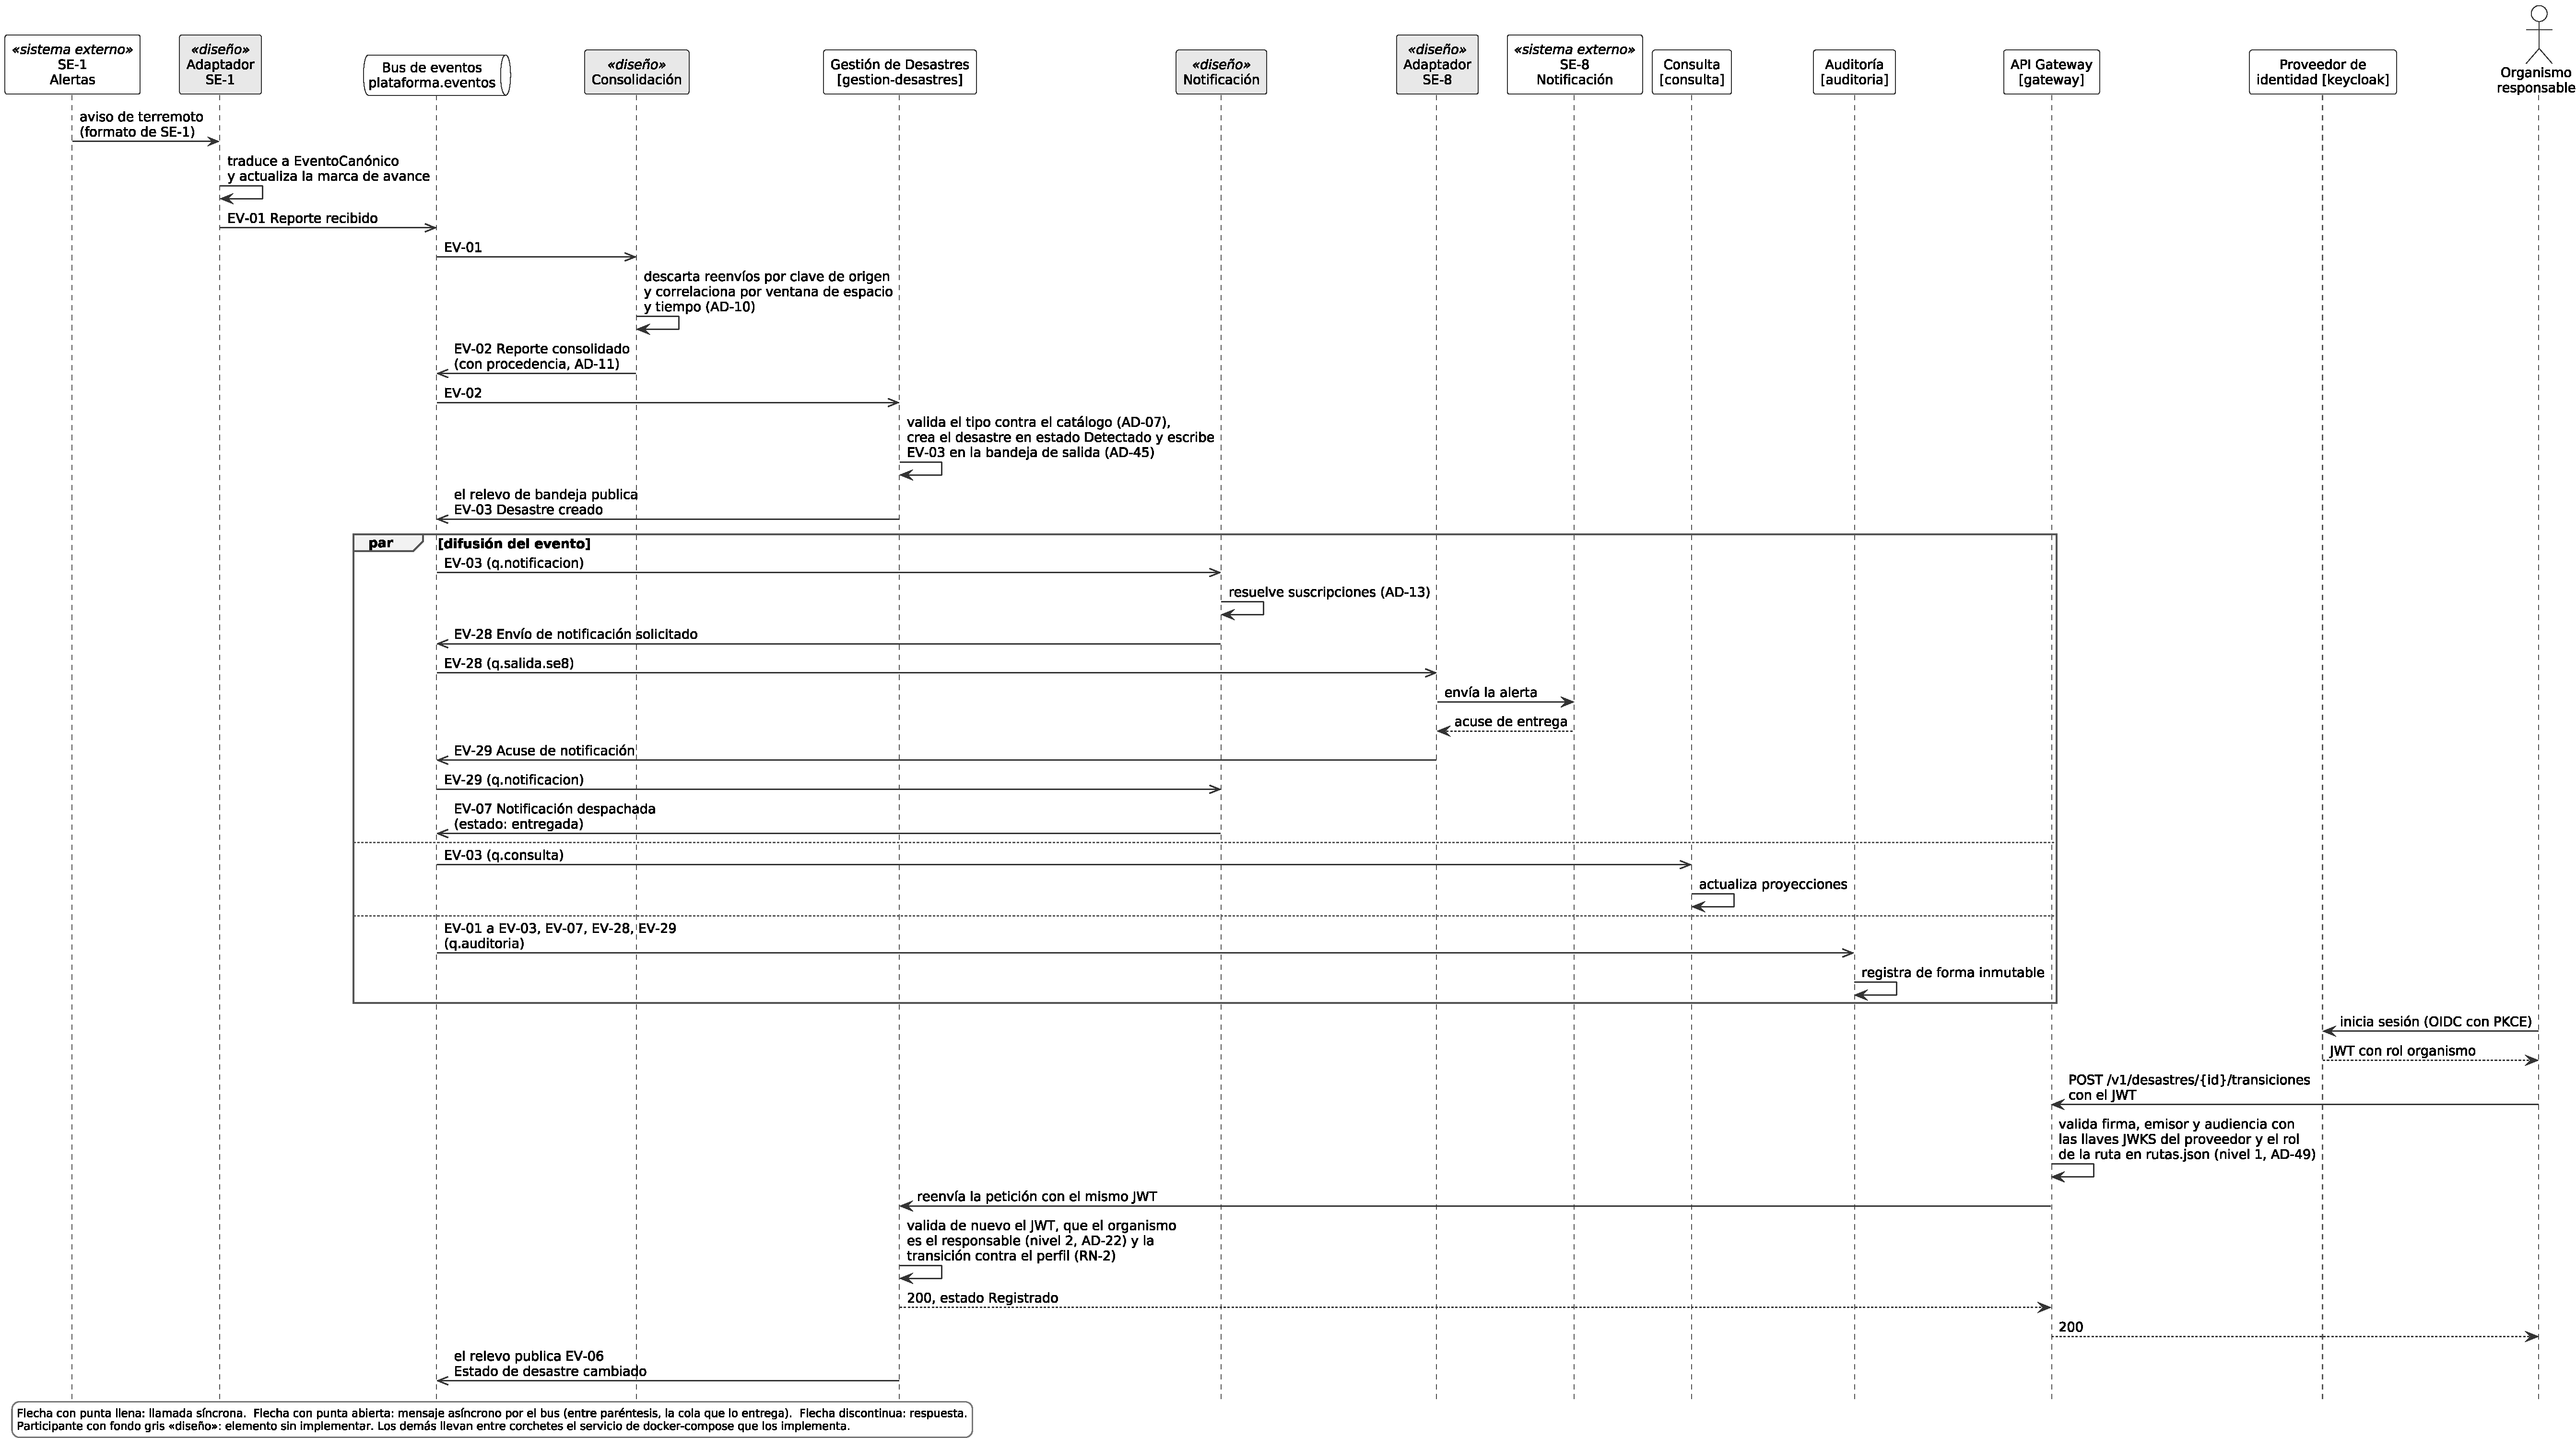
\includegraphics[width=\linewidth,height=0.86\textheight,keepaspectratio]{figuras/seq_eo1}
\caption{Diagrama de secuencia del inicio de una emergencia (SAD 1.2). Sustenta el
análisis de QA-09, QA-08 y QA-11.}
\label{fig:seq-eo1}
\end{figure}
\end{landscape}

\subsection{QA-14: Integridad de la sincronización sin conexión}
\label{sec:qa14}

\begin{longtable}{L{3.0cm} L{12.8cm}}
\cabecera{2}{tab:f-qa14}{Análisis de QA-14}{\textbf{Campo} & \textbf{Análisis}}
Escenario & Sincronización de 120 evaluaciones con 5 conflictos: 0 evaluaciones perdidas o
sobrescritas en silencio. Calificación (A, A), $P = 9$ \\
Enfoques & EA-16, réplica local, cola de operaciones y detección determinista sin resolución
automática. EA-19, bandeja de salida. EA-10, historial versionado. EA-11, auditoría de la decisión
humana. EA-22, registro idempotente con identificador del cliente. EA-26, umbrales y alarma de la
bandeja de revisión \\
Componentes impactados & Cliente móvil (réplica local y cola de operaciones), microservicio de
Evaluación de Daños y su almacén (historial, bandeja de revisión y bandeja de salida), Consulta de
Daños (marca en el mapa e indicadores de revisión, E-13) y Auditoría \\
Razonamiento & Se descartaron dos alternativas en la iteración 8: la resolución automática que
conserva el daño más alto y la regla de la última escritura. Ambas suponen que la plataforma puede
decidir qué versión se descarta. La plataforma no puede distinguir una reevaluación correcta de una
lectura errónea.\newline
La versión 1.0 del SAD exigía una regla determinista y no la definía. El SAD 1.1 la define en AD-43:
hay conflicto si el activo tiene una versión mayor que la versión base de la operación, producida
por otro dispositivo. La \cref{fig:seq-eo4} muestra la secuencia. La medida y la respuesta se
sostienen así:\newline
La medida, 0 evaluaciones perdidas o sobrescritas en silencio: ningún caso de tratamiento elimina una
versión (AD-32), y una operación solo sale de la cola local con respuesta del servidor (AD-44).\newline
La detección del \qty{100}{\percent} de los conflictos: todo cambio de otro dispositivo aumenta la
versión del activo, de modo que la regla lo detecta siempre.\newline
Los 0 duplicados en el reenvío: el servidor registra el identificador de cada operación y devuelve el
resultado guardado (AD-44).\newline
La bandeja de salida (EA-19) escribe EV-09 y EV-10 en la misma transacción que la evaluación. La
bandeja de revisión pertenece a Evaluación de Daños, porque resolver un conflicto exige consistencia
fuerte con la versión vigente (E-13). Consulta de Daños y Auditoría reciben todos los conflictos por
EV-10 (AD-45). La evidencia medida está en el \cref{tab:verificacion} \\
Sensibilidad & PS-04, amplitud de la ventana de tiempo de la detección de duplicados (AD-33). Una
ventana corta deja pasar duplicados reales. Una ventana amplia marca como posibles duplicados
evaluaciones legítimas. PS-15, umbrales de la bandeja de revisión. PS-17, traslape de la descarga
incremental (E-38) \\
Compromiso & T-03. Integridad frente a tiempo de cierre y carga de revisión humana. Una detección
más estricta produce más casos en la bandeja de revisión y evaluaciones que tardan más en
cerrarse \\
Riesgos & R-08, mitigado en parte. El escenario mide una proporción de conflictos del
\qty{4}{\percent}. Con cientos de equipos, esa proporción puede generar más conflictos de los que la
revisión humana procesa. La versión 1.1 no fijaba un límite ni una alarma para la bandeja. La
implementación compara el tamaño y la antigüedad de la bandeja con umbrales configurables (EA-26).
La alarma no llega a Auditoría (L-02, R-11).\newline
Riesgo cerrado: la comparación del número de versión sin considerar el dispositivo marcaría como
conflicto las secuencias de crear y editar de un mismo dispositivo sin conexión (falsos positivos).
AD-43 lo evita al considerar el dispositivo que produjo cada versión \\
No riesgos & Ninguna evaluación se pierde en la sincronización. En la versión 1.0 este no riesgo
dependía de un supuesto sobre el cliente. En la versión 1.1 es una decisión (AD-44): la cola local
conserva cada operación hasta la respuesta del servidor. El reenvío del lote no produce
duplicados \\
\end{longtable}

\begin{figure}[p]
\centering
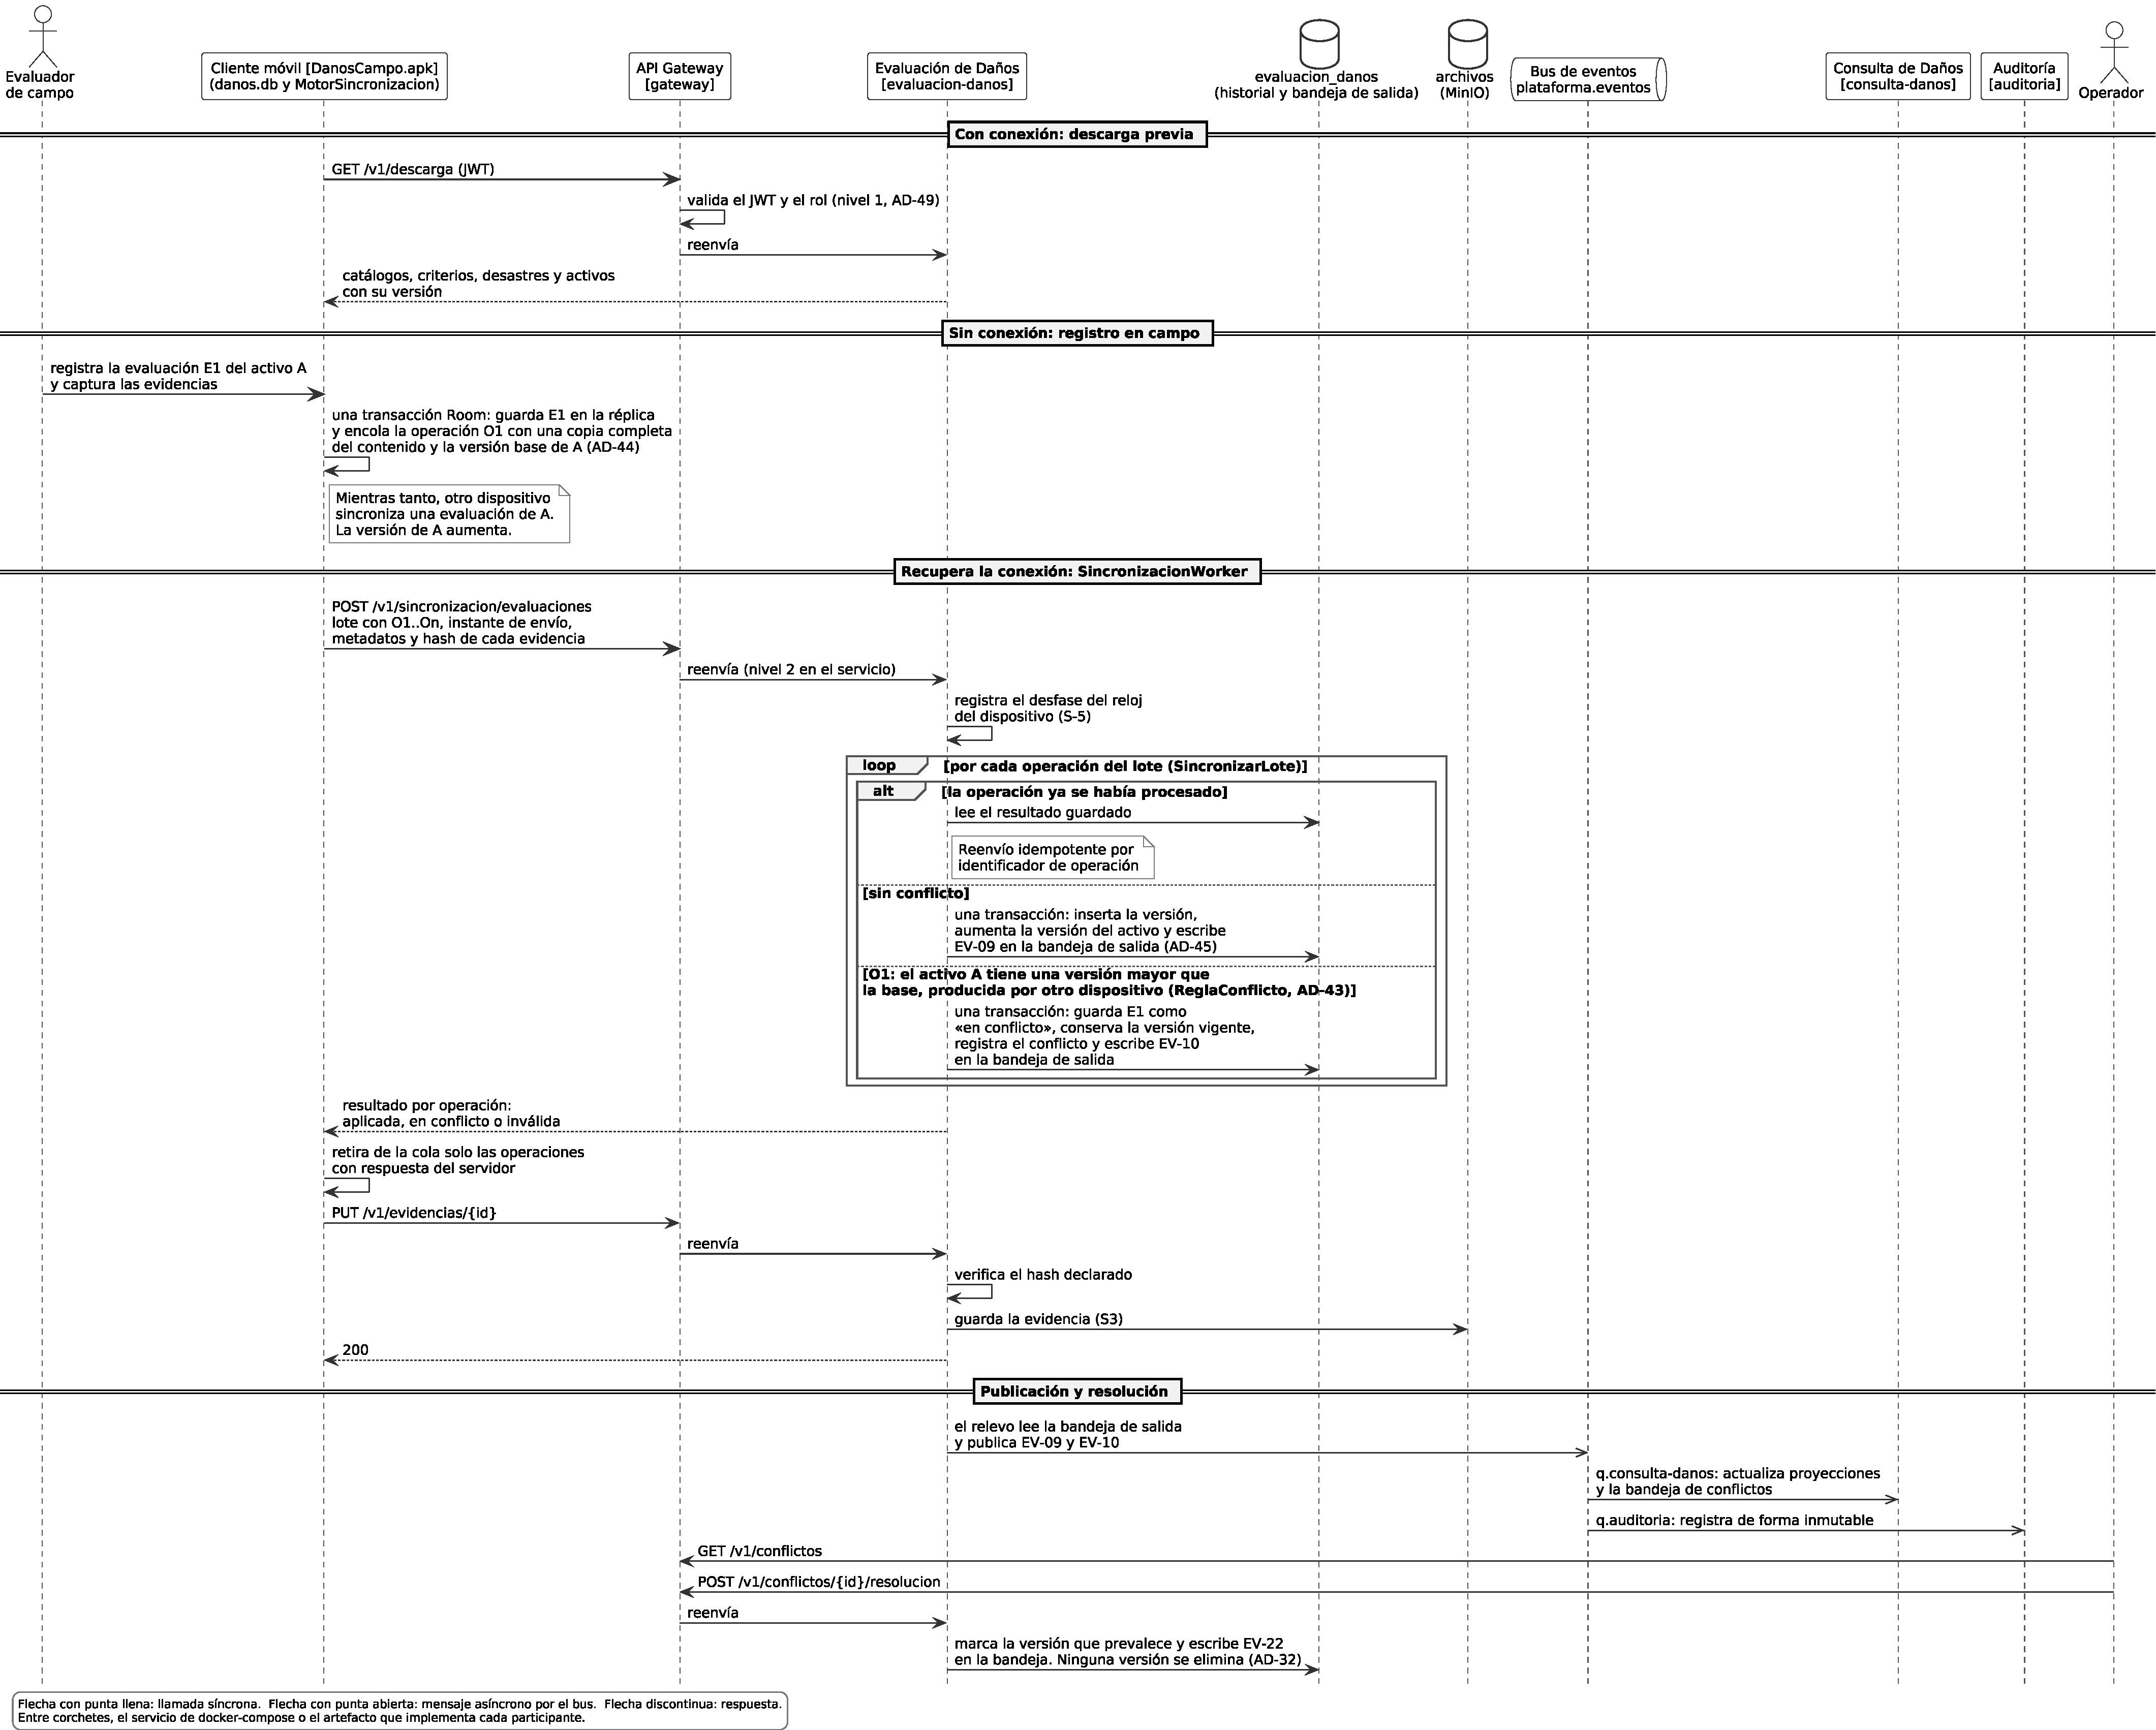
\includegraphics[width=\linewidth,height=0.9\textheight,keepaspectratio]{figuras/seq_eo4}
\caption{Diagrama de secuencia de la sincronización sin conexión con un conflicto (SAD 1.2).
Sustenta el análisis de QA-14.}
\label{fig:seq-eo4}
\end{figure}
\clearpage

\subsection{Análisis abreviado de las hojas con prioridad 6}
\label{sec:abreviado}

\subsubsection{QA-01: Fallo de un sistema externo}

\begin{longtable}{L{3.0cm} L{12.8cm}}
\cabecera{2}{tab:f-qa01}{Análisis de QA-01}{\textbf{Campo} & \textbf{Análisis}}
Escenario & SE-3 deja de responder durante una emergencia. Medida: 0 funciones que no dependen de SE-3
quedan indisponibles. Calificación (A, M), $P = 6$ \\
Enfoques & EA-05, EA-06, EA-18, EA-25 \\
Componentes impactados & Adaptador de SE-3, su cola de salida en el bus y el microservicio de
Consulta. En la implementación, el mismo mecanismo se verifica con los adaptadores de SE-6 y SE-7,
porque el de SE-3 no se implementó (L-06) \\
Razonamiento & El cortacircuitos aísla la indisponibilidad de SE-3 sin bloquear a los demás
componentes. La cola de salida conserva los mensajes pendientes. La marca de avance recupera el
rango pendiente cuando SE-3 vuelve, y el consumo idempotente evita duplicados. La consulta muestra
el último dato conocido con su marca de tiempo. La \cref{fig:seq-eo3} muestra la secuencia. El
mecanismo es el mismo en las ocho integraciones del SAD, y por eso la dificultad del escenario es
Media \\
Sensibilidad & PS-08, proporción de llamadas fallidas que abre el circuito y duración de cada tiempo
de espera. De ambos depende el plazo de \qty{30}{\second} de la respuesta de QA-01. PS-06 aplica
cuando el sistema caído es el de recursos (SE-4): de él depende cuánto tiempo queda retenida una
reserva sin confirmar (EA-17) \\
Compromiso & T-09: el mecanismo es el del contrato común de adaptador. T-04 en el caso de SE-4 \\
Riesgos & R-10, mitigado. La respuesta de QA-01 exige que la indisponibilidad de SE-3 se refleje en
el camino de consulta en \qty{30}{\second} o menos, con un indicador de que la fuente no responde. La
versión 1.1 no definía cómo el microservicio de Consulta conoce que el circuito se abrió. La
implementación agrega EV-23 (E-15): cada adaptador lo publica al abrir o cerrar el circuito, y lo
consumen Consulta, Consulta de Daños y Consulta del Programa (EA-25) \\
No riesgos & Las funciones que no dependen de SE-3 continúan, porque ninguna lo invoca de forma
síncrona (CON-3) \\
\end{longtable}

\begin{landscape}
\begin{figure}[p]
\centering
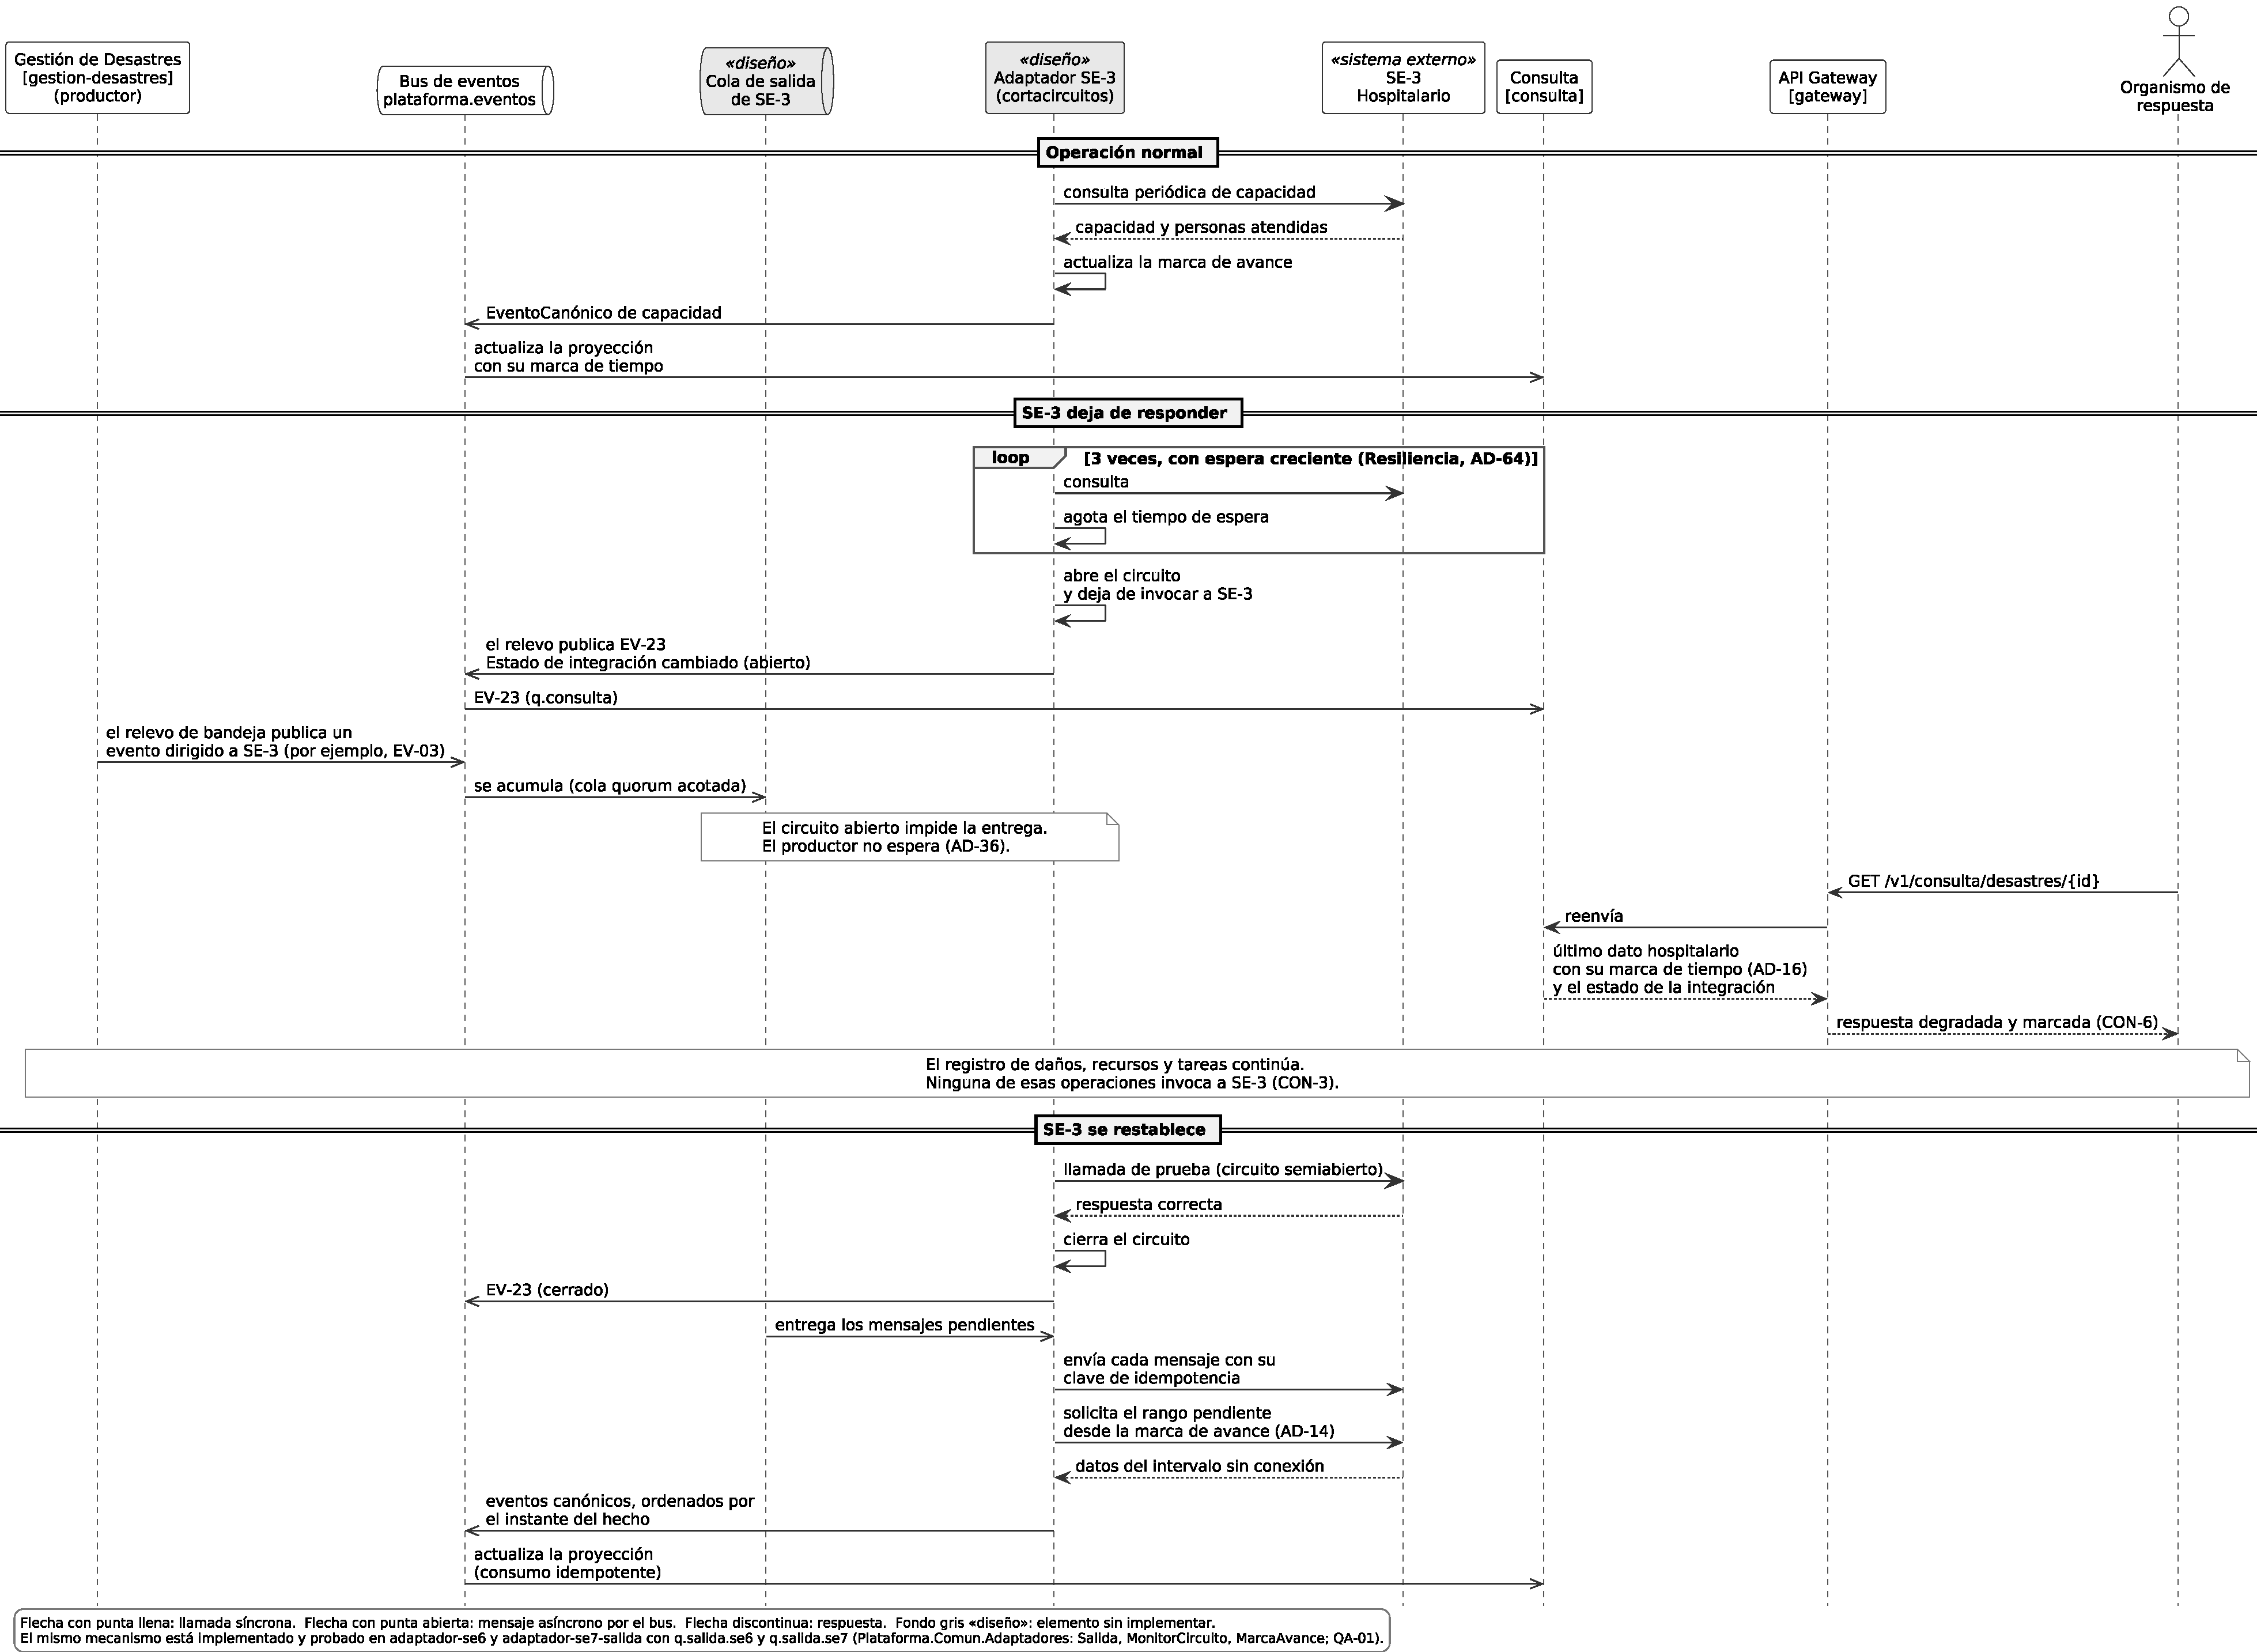
\includegraphics[width=\linewidth,height=0.86\textheight,keepaspectratio]{figuras/seq_eo3}
\caption{Diagrama de secuencia del fallo de SE-3 (SAD 1.2). Sustenta el análisis de
QA-01.}
\label{fig:seq-eo3}
\end{figure}
\end{landscape}

\subsubsection{QA-04: Fallo de un componente interno}

\begin{longtable}{L{3.0cm} L{12.8cm}}
\cabecera{2}{tab:f-qa04}{Análisis de QA-04}{\textbf{Campo} & \textbf{Análisis}}
Escenario & Un componente interno falla. Medida: 0 funciones críticas que no dependen de él quedan
indisponibles. Calificación (A, M), $P = 6$ \\
Enfoques & EA-02, EA-13, EA-18, EA-19, EA-21 \\
Componentes impactados & El microservicio afectado (el caso de referencia es Consolidación), su
cola en el bus y los microservicios que publican hacia él \\
Razonamiento & El bus desacopla al consumidor que falla del productor. Los mensajes dirigidos al
consumidor quedan en su cola hasta que se recupera. Las réplicas activas asumen la carga si falla
una instancia. La propagación se corta en \qty{60}{\second} o menos cuando los invocadores dejan de
generar peticiones hacia el componente afectado. La bandeja de salida (EA-19) cubre el caso en que
el bus no está disponible para cualquier microservicio productor (E-19). Una cola llena rechaza la
publicación y el evento permanece en la bandeja del productor. Un mensaje que falla cinco veces se
aparta a la cola de mensajes muertos del consumidor sin bloquear los siguientes (EA-21) \\
Sensibilidad & PS-14, umbral con el que los invocadores detectan el fallo (proporción de errores y
duración de la ventana). PS-16, largo máximo de cola y límite de entregas \\
Compromiso & T-10. La cola acotada con rechazo de publicación favorece 0 eventos perdidos y
aumenta la antigüedad del dato mientras la cola está llena (QA-06) \\
Riesgos & R-09, en lo que respecta a los eventos en tránsito durante una conmutación regional \\
No riesgos & No se pierden eventos encolados, mientras la retención del bus cubra el tiempo de
recuperación del consumidor. Una cola llena no descarta eventos, mientras la bandeja de salida del
productor los conserve hasta que la cola los acepte \\
\end{longtable}

\subsubsection{QA-05: Aumento repentino de usuarios}

\begin{longtable}{L{3.0cm} L{12.8cm}}
\cabecera{2}{tab:f-qa05}{Análisis de QA-05}{\textbf{Campo} & \textbf{Análisis}}
Escenario & La concurrencia pasa de \num{1000} a \num{10000} usuarios en \qty{10}{\minute}. Medida: consulta
frecuente en p95 $<$ \qty{2}{\second}. Calificación (A, M), $P = 6$ \\
Enfoques & EA-08, EA-15, EA-04 \\
Componentes impactados & API Gateway y los tres microservicios de consulta con sus proyecciones. Los
microservicios de escritura no cambian su capacidad \\
Razonamiento & El paso de \num{1000} a \num{10000} usuarios se atiende con más réplicas de los
procesos de consulta (EA-08), sin cambio de código ni redespliegue. El API Gateway prioriza la
consola de coordinación sobre el portal público si la carga supera la capacidad (EA-04) \\
Sensibilidad & PS-05, retardo de propagación de los eventos del bus hacia las proyecciones \\
Compromiso & T-01. Escalabilidad frente a consistencia: la separación de lectura y escritura
introduce un retraso de hasta \qty{2}{\second} entre un cambio y su consulta \\
Riesgos & Ninguno identificado \\
No riesgos & La consulta se mantiene dentro de su objetivo, mientras el incremento de réplicas se
complete en \qty{5}{\minute} o menos \\
\end{longtable}

\subsubsection{QA-08: Latencia de la cadena de alerta}

\begin{longtable}{L{3.0cm} L{12.8cm}}
\cabecera{2}{tab:f-qa08}{Análisis de QA-08}{\textbf{Campo} & \textbf{Análisis}}
Escenario & Un desastre pasa a Nivel\_3 o Nivel\_4. Medida: alerta crítica entregada con p95 $<$
\qty{5}{\second}. Calificación (A, M), $P = 6$ \\
Enfoques & EA-02, EA-15 \\
Componentes impactados & Gestión de Desastres, bus de eventos, Notificación y adaptador de SE-8
(\cref{fig:seq-eo1}) \\
Razonamiento & El bus entrega el evento a Notificación sin que el productor espere. El adaptador de
SE-8 envía la alerta y recibe el acuse \\
Sensibilidad & PS-09, tiempo de arranque de un adaptador efímero \\
Compromiso & Ninguno adicional \\
Riesgos & R-01. El arranque de un adaptador efímero que no se ha invocado recientemente puede
exceder \qty{5}{\second}. La mitigación está decidida en AD-25: mantener una instancia encendida del
adaptador de SE-8. Notificación y el adaptador de SE-8 quedan fuera de la implementación (L-06), por
lo que la mitigación sigue sin verificar \\
No riesgos & Una alerta no se da por entregada sin acuse, porque Notificación conserva el estado de
entrega (AD-13) \\
\end{longtable}

\subsubsection{QA-11: Autorización por organización}

\begin{longtable}{L{3.0cm} L{12.8cm}}
\cabecera{2}{tab:f-qa11}{Análisis de QA-11}{\textbf{Campo} & \textbf{Análisis}}
Escenario & Un organismo no responsable intenta modificar un desastre ajeno. Medida: \qty{100}{\percent} de
rechazos sobre al menos 200 casos. Calificación (A, M), $P = 6$ \\
Enfoques & EA-12, EA-23, EA-24 \\
Componentes impactados & Proveedor de identidad, API Gateway (nivel 1) y el microservicio de
destino (nivel 2). En el caso de referencia, Gestión de Desastres \\
Razonamiento & La medida exige un \qty{100}{\percent} de rechazos a un organismo no responsable. El
API Gateway valida el rol general. El microservicio valida que el organismo sea el responsable
asignado del desastre. Ninguno de los dos niveles alcanza por separado el \qty{100}{\percent} de
rechazos: el API Gateway no conoce la relación entre el organismo y el desastre, y la validación
solo en el microservicio deja sin protección las rutas que no la implementen.\newline
En la implementación, el gateway valida el catálogo de rutas al arrancar y no arranca si una ruta de
modificación no declara su regla de dominio (EA-23). Cada microservicio valida otra vez el token
(EA-24). Fuera de su jurisdicción, una autoridad recibe 404 y no 403 (E-39) \\
Sensibilidad & Ninguna de valor numérico. La medida depende de que toda ruta de modificación
aplique los dos niveles \\
Compromiso & T-11, confidencialidad frente a diagnóstico (404 en vez de 403). T-12, defensa en
profundidad frente a dependencia del emisor del token \\
Riesgos & R-07, mitigado con residuo: una ruta que declara la regla \texttt{ninguna} pasa la
validación del catálogo. R-11: los rechazos no llegan a Auditoría, por lo que no se cumple el registro
del intento que pide la respuesta (L-02). R-12: sin cifrado entre servicios. R-13: llaves y emisor del token \\
No riesgos & Un organismo no responsable no modifica un desastre ajeno, mientras toda ruta de
modificación declare su regla de dominio en el catálogo. La evidencia medida está en el
\cref{tab:verificacion} \\
\end{longtable}

\subsubsection{QA-12: Protección de datos personales}

\begin{longtable}{L{3.0cm} L{12.8cm}}
\cabecera{2}{tab:f-qa12}{Análisis de QA-12}{\textbf{Campo} & \textbf{Análisis}}
Escenario & Alguien sin necesidad de conocer intenta leer los datos de personas afectadas. Medida:
\qty{100}{\percent} de los campos identificatorios ilegibles sin la clave. Calificación (A, M),
$P = 6$ \\
Enfoques & EA-12 \\
Componentes impactados & Microservicio de Personas Afectadas, su almacén y el adaptador de SE-5 \\
Razonamiento & Los campos identificatorios se cifran por columna y son ilegibles sin la clave. Los
roles sin necesidad de conocer reciben información agregada o seudonimizada \\
Sensibilidad & PS-07, lista de columnas declaradas como sensibles \\
Compromiso & T-05. Seguridad frente a rendimiento: el cifrado por columna no penaliza las consultas
frecuentes, pero no protege un campo sensible que no se haya declarado \\
Riesgos & R-06, en lo que respecta a la eliminación de datos personales (ES-05). R-12, en lo que
respecta al tráfico sin cifrar entre servicios \\
No riesgos & Una copia de respaldo no expone datos identificatorios, mientras las claves se
almacenen fuera del almacén cifrado \\
\end{longtable}

\subsection{Análisis resumido de las hojas con prioridad de 2 a 4}
\label{sec:resumido}

El \cref{tab:resumido} indica, para las cinco hojas de menor prioridad, los enfoques, los puntos de
sensibilidad, los compromisos y los riesgos. En la versión 1.0 estas hojas se declaraban cubiertas
sin análisis.

\begin{longtable}{L{1.3cm} L{2.4cm} L{5.4cm} L{3.0cm} L{3.0cm}}
\cabecera{5}{tab:resumido}{Análisis resumido de QA-06, QA-07, QA-10, QA-13 y QA-15}{\textbf{ID} &
\textbf{Enfoques} & \textbf{Razonamiento} & \textbf{Sensibilidad y compromiso} & \textbf{Riesgos y
no riesgos}}
QA-06 & EA-08, EA-09 & La consulta se atiende con proyecciones y con la caché de geometrías, sin
cálculo en cada petición & PS-05, PS-07, PS-16. T-01, T-05 y T-10 & R-14. No riesgo: la latencia se
mantiene mientras EV-05 invalide la caché de Consulta, y EV-21 y los eventos de evaluación la de
Consulta de Daños (E-21) \\
QA-07 & EA-01, EA-08, EA-22 & El registro escribe en un solo almacén y no espera a los
consumidores ni a la región secundaria. Un reenvío desde la app con el mismo identificador devuelve
el desastre ya registrado (AD-48) & PS-02. T-02 & Sin riesgos. No riesgo: la escritura no espera la
replicación \\
QA-10 & EA-07 & El tipo de desastre es una entrada del catálogo, con su perfil de ciclo de vida y
sus criterios & Sin punto de sensibilidad numérico & Sin riesgos. No riesgo: no se modifican
componentes mientras la variabilidad sea de datos y no de comportamiento \\
QA-13 & EA-10, EA-11, EA-20 & Auditoría persiste los eventos de cambio en un registro de solo
inserción y detecta los huecos en la secuencia de cada productor & PS-11. T-07 & R-02 (mitigado),
R-06 y R-11. No riesgo: el rastro se reconstruye con una consulta, y un evento ausente se señala
como hueco \\
QA-15 & EA-10, EA-11, EA-19 & El historial de solo inserción conserva cada cambio de presupuesto y
de estado. La bandeja de salida de Reconstrucción publica el cambio en la misma transacción &
Sin punto de sensibilidad numérico. Sin compromiso & R-02 (mitigado). No riesgo: una entrada no se
modifica, porque el almacén no admite actualización ni borrado \\
\end{longtable}

%==============================================================================
\newpage
\section{Paso 7. Lluvia de escenarios y repriorización}
\label{sec:paso7}

Este paso propone escenarios que el diseño no previó, para comprobar si los enfoques existentes los
atienden. El equipo propuso los seis escenarios del \cref{tab:lluvia}. Cada uno se califica con la escala del
paso 5. La calificación es una valoración del equipo: la importancia indica el efecto sobre los drivers
de negocio, y la dificultad, el esfuerzo de atenderlo con los enfoques existentes. Se analizan en el
paso 8 los escenarios con $P \ge 6$.

\begin{longtable}{L{1.3cm} L{9.0cm} C{1.2cm} C{0.6cm} L{2.8cm}}
\cabecera{5}{tab:lluvia}{Escenarios propuestos en el paso 7}{\textbf{ID} & \textbf{Escenario} &
\textbf{(I, D)} & \textbf{P} & \textbf{Resultado}}
ES-01 & Dos desastres de Nivel\_4 ocurren al mismo tiempo en regiones distintas. La carga crítica se
duplica & (A, B) & 3 & Descartado \\
ES-02 & Un organismo participante se retira de la respuesta durante la emergencia. Quedan sus
tareas, sus recursos reservados y su responsabilidad sobre un desastre & (M, B) & 2 & Descartado \\
ES-03 & Un sistema externo responde, pero entrega datos corruptos o inverosímiles. El
cortacircuitos no se abre & (A, M) & 6 & Analizado en el paso 8 \\
ES-04 & La región secundaria falla mientras la primaria no está disponible & (A, B) & 3 & Descartado \\
ES-05 & Una norma obliga a eliminar los datos personales de una persona afectada, y el registro de
auditoría es inmutable & (A, M) & 6 & Analizado en el paso 8 \\
ES-06 & Se incorpora un noveno sistema externo cuyo protocolo o modelo de datos no se ajusta al
contrato de adaptador & (A, M) & 6 & Analizado en el paso 8 \\
\end{longtable}

Se descartaron tres escenarios:

\begin{itemize}
  \item ES-01. La priorización del API Gateway y la elasticidad del modelo de lectura atienden los
        picos de carga con independencia del número de desastres que los originan (EA-04, EA-08).
  \item ES-02. El escenario corresponde a reglas de negocio sobre la reasignación de tareas y de
        recursos. No requiere un mecanismo arquitectónico distinto de los existentes.
  \item ES-04. La ficha de QA-03 ya define la respuesta: restauración desde copia de respaldo en
        \qty{4}{\hour} o menos, con un RPO de \qty{24}{\hour} o menos.
\end{itemize}

El árbol de utilidad no cambia. ES-03 y ES-06 ponen a prueba enfoques ya analizados: ES-03 presiona
sobre QA-01 (EA-05) y ES-06 sobre QA-09 (EA-03). ES-05 no corresponde a una hoja del árbol. Es una
tensión entre dos decisiones de seguridad (AD-23 y AD-41) y se analiza en el paso 8 como hallazgo.

%==============================================================================
\section{Paso 8. Análisis de los enfoques resultantes}
\label{sec:paso8}

La \cref{fig:impactados} muestra los componentes que impacta cada uno de los tres escenarios
analizados. Cada ficha repite esos componentes en su fila correspondiente.

\begin{landscape}
\begin{figure}[p]
\centering
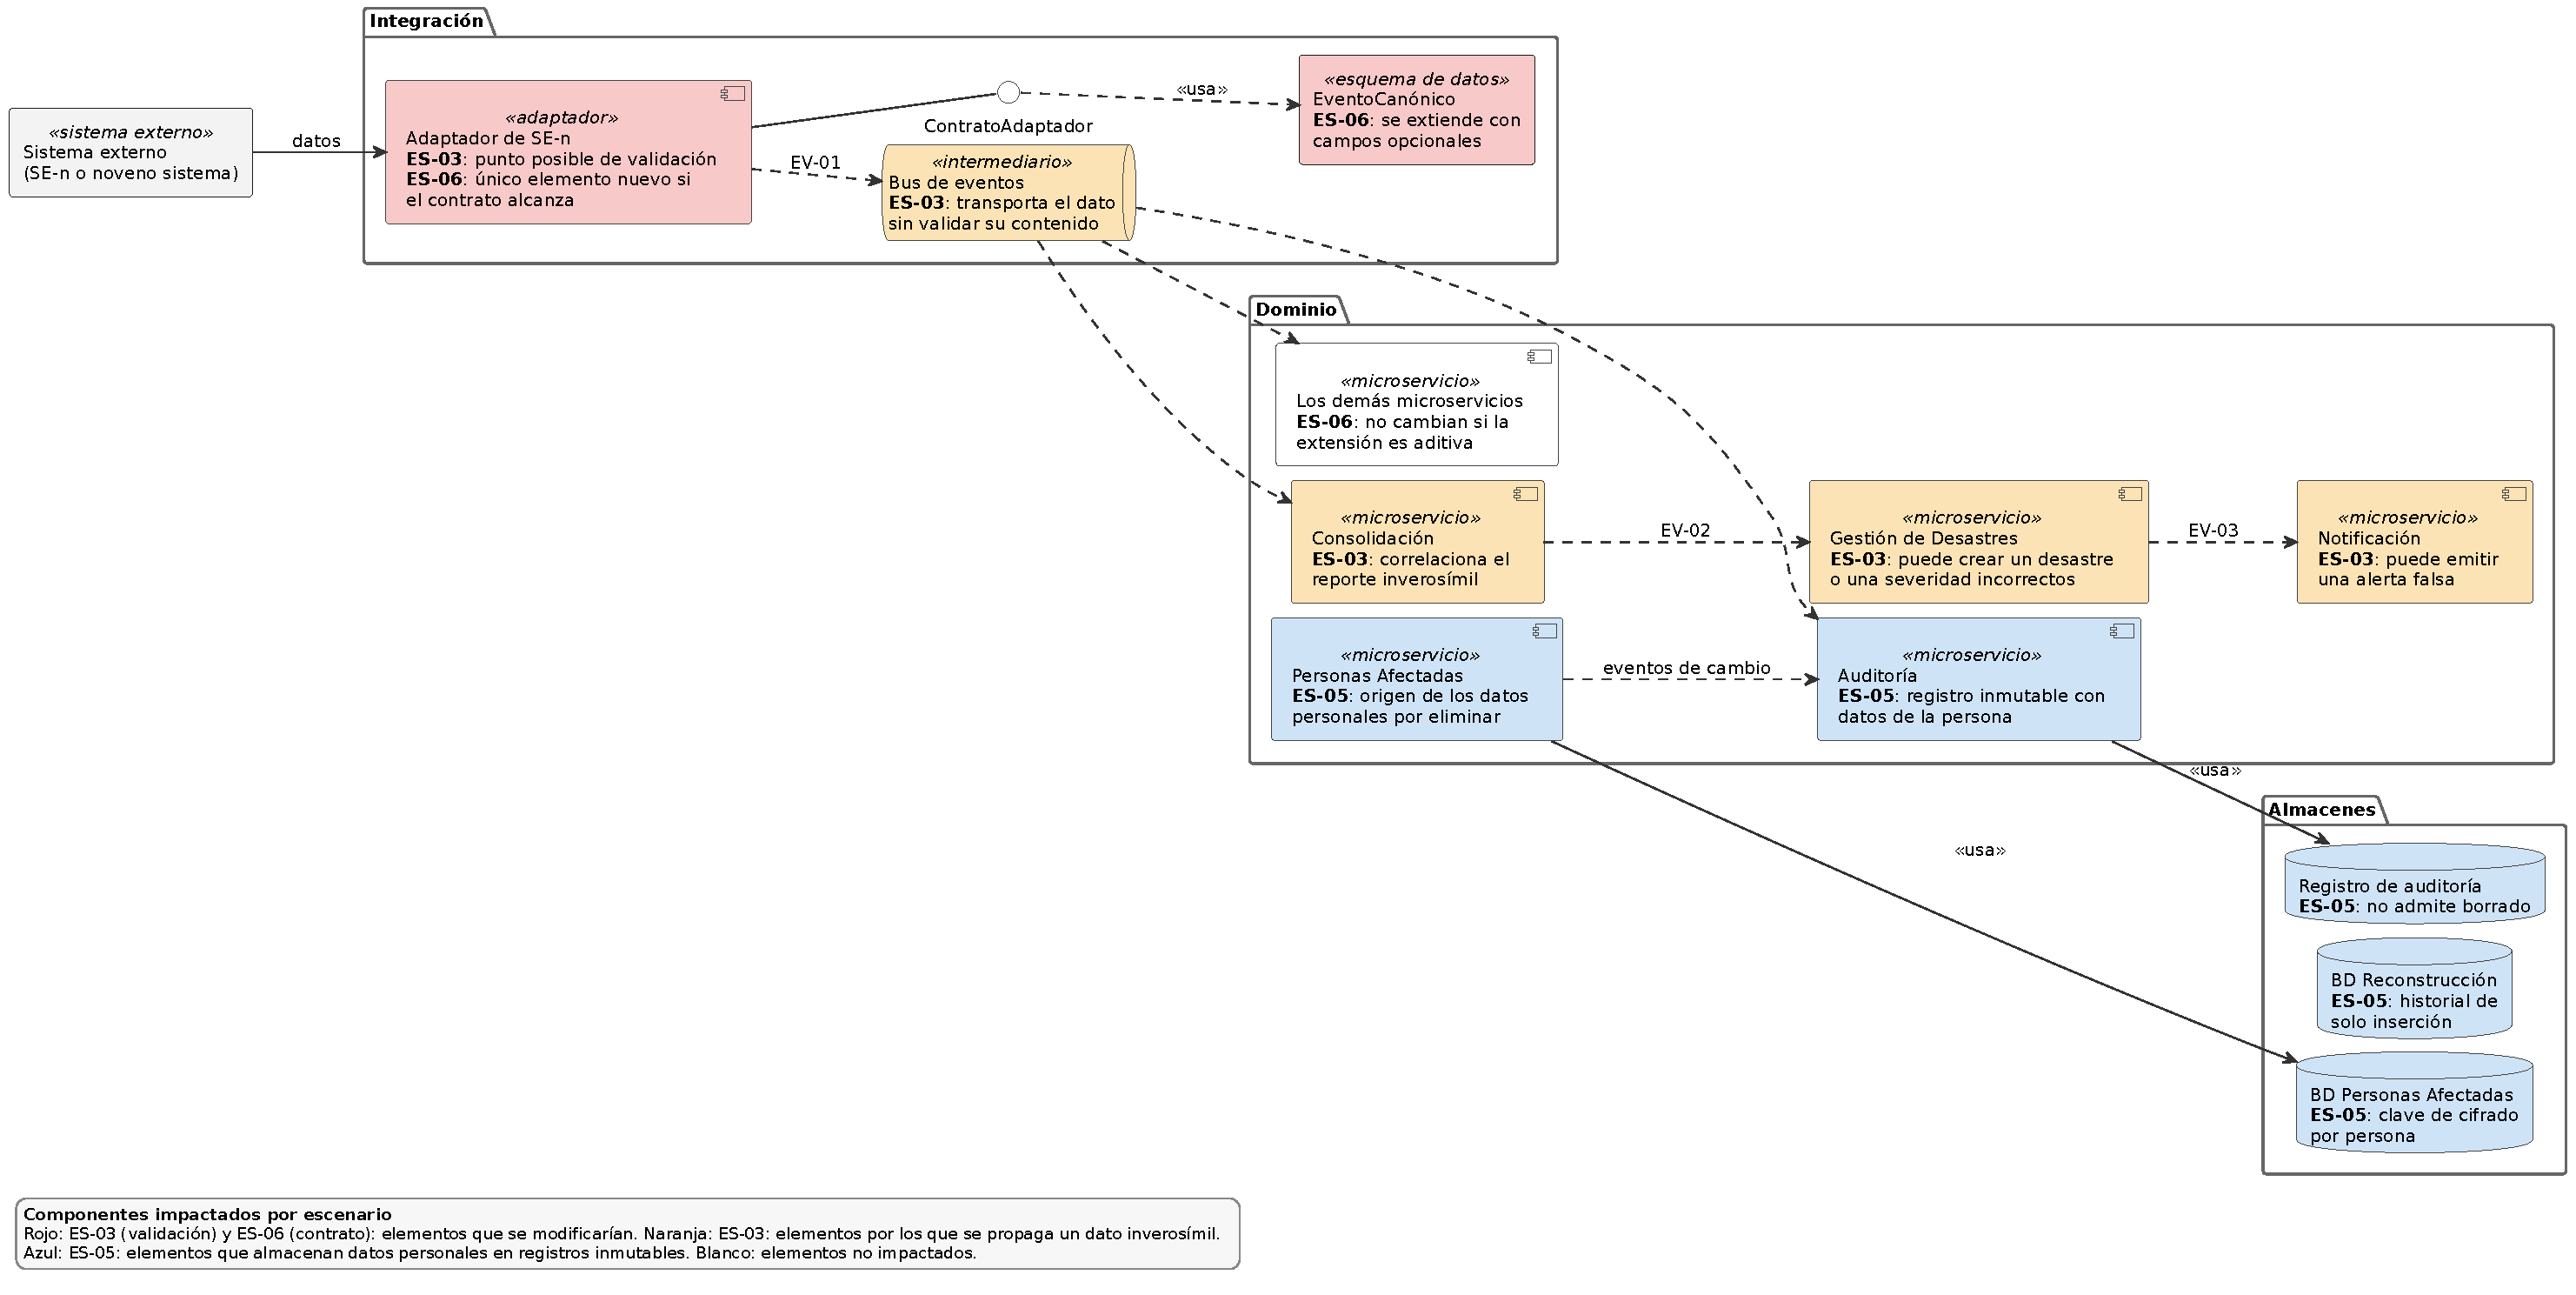
\includegraphics[width=\linewidth,height=0.86\textheight,keepaspectratio]{figuras/componentes_impactados}
\caption{Componentes impactados por los escenarios ES-03, ES-05 y ES-06.}
\label{fig:impactados}
\end{figure}
\end{landscape}

\subsection{ES-03: Datos corruptos o inverosímiles de un sistema externo que responde}

\begin{longtable}{L{3.0cm} L{12.8cm}}
\cabecera{2}{tab:f-es03}{Análisis de ES-03}{\textbf{Campo} & \textbf{Análisis}}
Escenario & Un sistema externo responde con normalidad y el cortacircuitos no se abre. Los valores
que entrega son inverosímiles: una magnitud sísmica fuera de rango o unas coordenadas en el mar para
una ubicación en tierra \\
Enfoques & Ningún enfoque del \cref{tab:enfoques} cubre el caso. EA-05 observa la ausencia de
respuesta o el error, y no el contenido. EA-03 valida que el mensaje se traduzca al evento canónico,
y no que sus valores sean verosímiles \\
Componentes impactados & El dato entra por el adaptador del sistema externo y se propaga por el bus
de eventos a Consolidación, Gestión de Desastres y Notificación. Una validación se ubicaría en el
adaptador o en la entrada al bus (\cref{fig:impactados}) \\
Razonamiento & Los mecanismos de resiliencia suponen que la indisponibilidad se manifiesta como
ausencia de respuesta o como error. Un sistema que responde con datos erróneos no activa ninguno.
El dato inverosímil se publica como EV-01, se consolida y puede originar un desastre o una
clasificación de severidad incorrectos \\
Sensibilidad & PS-10. Dos parámetros afectan los mismos atributos. El primero es la ubicación de la
validación: en el adaptador, que conoce el dominio del sistema de origen, o en la entrada al bus,
que es común y no conoce el contexto. El segundo es la severidad de la regla: una regla estricta
rechaza más datos erróneos y también más datos legítimos extremos, que en un desastre pueden ser el
primer indicio de un evento grave \\
Compromiso & T-06. Validar el contenido afecta QA-09: cada regla de plausibilidad es específica del
dominio y del sistema, lo que reduce la generalidad del contrato común que AD-09 buscó \\
Riesgos & R-05. La arquitectura no distingue un dato erróneo bien formado de uno correcto. Un
reporte corrupto se propaga con la misma confianza que uno legítimo \\
No riesgos & Ninguno \\
\end{longtable}

\subsection{ES-05: Eliminación de datos personales en un registro inmutable}

\begin{longtable}{L{3.0cm} L{12.8cm}}
\cabecera{2}{tab:f-es05}{Análisis de ES-05}{\textbf{Campo} & \textbf{Análisis}}
Escenario & Una persona afectada ejerce su derecho a la eliminación de sus datos personales. El
registro de auditoría (AD-21) y el historial de solo inserción (AD-41) no admiten borrado \\
Enfoques & EA-11, auditoría centralizada, y EA-12, cifrado por columna, que entran en tensión.
EA-10, historial de solo inserción \\
Componentes impactados & Microservicio de Personas Afectadas y su almacén, microservicio de
Auditoría y registro de auditoría, y almacén de Reconstrucción (\cref{fig:impactados}) \\
Razonamiento & Las dos decisiones son correctas por separado. La inmutabilidad impide borrar la
evidencia de una operación crítica, y el derecho a la eliminación exige borrar. AD-23 decide cifrar por
columna, pero no define cuántas claves se usan. Este análisis propone una salida que respeta ambas
decisiones: cifrar los datos de cada persona con una clave propia, de modo que eliminarlos consista en
destruir esa clave. El registro de que ocurrió una operación sobre esa persona en una fecha se
conserva, y el contenido personal queda ilegible. La clave por persona es una propuesta de esta
evaluación: el SAD no la ha adoptado \\
Sensibilidad & PS-11, granularidad de las claves de cifrado, que el SAD no define. Con una clave
única para todos los registros, destruirla afecta a todas las personas. La eliminación selectiva
exigiría una clave por persona \\
Compromiso & T-07. Trazabilidad frente a cumplimiento normativo. La destrucción de la clave conserva
el rastro de la operación y pierde la posibilidad de auditar después su contenido \\
Riesgos & R-06. Ni el SAD ni las iteraciones de ADD definen un mecanismo de eliminación de datos
personales dentro de un registro inmutable \\
No riesgos & Ninguno \\
\end{longtable}

\subsection{ES-06: Un noveno sistema que no se ajusta al contrato}

\begin{longtable}{L{3.0cm} L{12.8cm}}
\cabecera{2}{tab:f-es06}{Análisis de ES-06}{\textbf{Campo} & \textbf{Análisis}}
Escenario & Se requiere incorporar un sistema externo cuyo protocolo o modelo de datos no se ajusta
al contrato de adaptador ni al evento canónico vigentes \\
Enfoques & EA-03, contrato de adaptador y evento canónico \\
Componentes impactados & El adaptador nuevo y el esquema \texttt{EventoCanónico}. Si la extensión es
aditiva, los ocho adaptadores y los doce microservicios no cambian (\cref{fig:impactados}) \\
Razonamiento & Hay dos opciones. La primera es extender el contrato con campos opcionales, sin
eliminar ni renombrar los existentes. No afecta a los ocho adaptadores, pero modifica un elemento
común, que es el costo que AD-09 declaró. La segunda es aceptar un adaptador que no cumple el
contrato completo. Esta opción obliga a que algún microservicio de dominio conozca el caso
especial, lo que elimina la abstracción que sustenta QA-09 \\
Sensibilidad & PS-12, naturaleza del cambio del contrato. Si el cambio agrega campos opcionales, el
costo es bajo. Si cambia el significado de un campo existente, afecta a los ocho adaptadores \\
Compromiso & T-09. Interoperabilidad frente a estabilidad del contrato común. El escenario confirma
el compromiso que AD-09 declaró \\
Riesgos & R-03. La medida de 0 componentes modificados de QA-09 puede incumplirse \\
No riesgos & Extender el contrato no modifica los ocho adaptadores existentes, mientras la extensión
se limite a campos opcionales y ningún campo cambie de significado \\
\end{longtable}

%==============================================================================
\newpage
\section{Paso 9. Presentación de resultados}
\label{sec:paso9}

\subsection{Puntos de sensibilidad}
\label{sec:sensibilidad}

El \cref{tab:sensibilidad} consolida los puntos de sensibilidad identificados en los pasos 6 y 8.
Cada uno indica la propiedad, el escenario cuya medida depende de ella y el efecto de modificarla.
Los puntos que afectan a más de un atributo en sentidos opuestos son además puntos de compromiso, y
la última columna los relaciona con el \cref{tab:tradeoffs}. PS-15 a PS-17 se agregan en la
versión 1.2: son parámetros que la implementación fija con un valor concreto.

\begin{longtable}{L{1.2cm} L{4.2cm} L{1.9cm} L{5.5cm} L{2.5cm}}
\cabecera{5}{tab:sensibilidad}{Puntos de sensibilidad}{\textbf{ID} & \textbf{Propiedad} &
\textbf{Escenario} & \textbf{Efecto de modificarla} & \textbf{Compromiso}}
PS-01 & Número de réplicas activas por microservicio & QA-02 & Determina cuántos fallos simultáneos
de instancia se toleran & Ninguno \\
PS-02 & Retardo de la replicación asíncrona entre regiones & QA-03, QA-07 & Si se acerca a
\qty{60}{\second}, el RPO real incumple la medida & T-02 \\
PS-03 & Expresividad del contrato de adaptador y del evento canónico & QA-09 & Un contrato estrecho
excluye sistemas. Uno amplio aumenta la complejidad de cada adaptador & T-09 \\
PS-04 & Amplitud de la ventana de detección de duplicados & QA-14 & Una ventana corta omite
duplicados. Una amplia aumenta la revisión humana & T-03 \\
PS-05 & Retardo de propagación de los eventos hacia las proyecciones & QA-05, QA-06 & Si crece, la
consulta muestra datos más antiguos sin que ocurra un fallo & T-01 \\
PS-06 & Plazo de expiración de la reserva de recursos & QA-01 & Un plazo largo retiene recursos sin
confirmar. Uno corto libera reservas válidas & T-04 \\
PS-07 & Lista de columnas declaradas como sensibles & QA-12, QA-06 & Menos columnas reducen el
costo de consulta y la cobertura del cifrado & T-05 \\
PS-08 & Proporción de llamadas fallidas que abre el circuito y duración de cada tiempo de espera &
QA-01 &
Determina el plazo en el que se detecta la indisponibilidad de un sistema externo & Ninguno \\
PS-09 & Tiempo de arranque de un adaptador efímero & QA-08 & Si excede el margen, la alerta crítica
supera los \qty{5}{\second} & Ninguno \\
PS-10 & Ubicación y severidad de la validación de plausibilidad & ES-03, QA-09 & Una validación
estricta rechaza datos legítimos extremos y reduce la generalidad del contrato & T-06 \\
PS-11 & Granularidad de las claves de cifrado, que el SAD no define & ES-05, QA-13 & Una clave por
persona, propuesta en ES-05, permitiría la eliminación selectiva & T-07 \\
PS-12 & Naturaleza del cambio del contrato: aditivo o semántico & ES-06, QA-09 & Un cambio semántico
afecta a los ocho adaptadores & T-09 \\
PS-13 & Valor del RTO de la conmutación regional & QA-02, QA-03 & Un RTO menor exige una segunda
región activa & T-08 \\
PS-14 & Umbral con el que los invocadores detectan el fallo de un componente & QA-04 & Un umbral
alto retrasa el corte de la propagación. Uno bajo produce cortes por fallos transitorios &
Ninguno \\
PS-15 & Umbrales de la bandeja de revisión: tamaño y antigüedad del conflicto más antiguo (50
conflictos y \qty{24}{\hour} por omisión) & QA-14 & Un umbral alto retrasa la alarma y deja crecer
la bandeja. Uno bajo produce alarmas que no exigen acción & T-03 \\
PS-16 & Largo máximo de cola (\num{100000} mensajes y \qty{256}{\mebi\byte}) y límite de 5 entregas
(\texttt{delivery-limit} de la política \texttt{plataforma-colas}) & QA-04, QA-06 & Una cola corta
se llena antes y retiene eventos en la bandeja del productor, lo que aumenta la antigüedad del dato.
Un límite bajo aparta mensajes con fallos transitorios. Uno alto retrasa los mensajes siguientes &
T-10 \\
PS-17 & Traslape de \qty{60}{\second} de la descarga incremental (E-38) & QA-14 & Un traslape
corto omite cambios confirmados después de leer el reloj. Uno largo repite activos en cada descarga
& Ninguno \\
\end{longtable}

\subsection{Puntos de compromiso}
\label{sec:compromisos}

Los cinco primeros compromisos estaban declarados en las decisiones del SAD como costo aceptado.
T-06 y T-07 resultan del paso 8. T-08 resulta de analizar en conjunto QA-02 y QA-03. T-09 estaba
declarado en AD-09. T-10 a T-12 se agregan en la versión 1.2 y resultan de decisiones que la
implementación hizo explícitas.

\begin{longtable}{L{1.05cm} L{3.2cm} L{4.3cm} L{4.5cm} L{1.6cm}}
\cabecera{5}{tab:tradeoffs}{Puntos de compromiso}{\textbf{ID} & \textbf{Decisión} & \textbf{Atributo
favorecido} & \textbf{Atributo afectado} & \textbf{PS}}
T-01 & AD-15. Separación del modelo de lectura y del de escritura & Escalabilidad: la consulta se
replica sin replicar la escritura (QA-05) & Consistencia inmediata: retraso objetivo menor que
\qty{2}{\second} & PS-05 \\
T-02 & AD-26. Replicación asíncrona entre regiones & Latencia de escritura (QA-07) y continuidad
regional (QA-02) & RPO de hasta \qty{60}{\second}: pérdida acotada de datos ante un siniestro
(QA-03) & PS-02 \\
T-03 & AD-32. Detección de conflictos sin resolución automática & Integridad: 0 evaluaciones perdidas o
sobrescritas en silencio (QA-14) & Tiempo de cierre de la evaluación y carga de revisión humana &
PS-04 \\
T-04 & AD-39. Reserva optimista con plazo de expiración & Disponibilidad: la asignación no espera
al sistema externo (QA-01) & Exactitud transitoria: una solicitud puede tardar hasta el plazo en
conocerse como rechazada & PS-06 \\
T-05 & AD-23. Cifrado por columna & Rendimiento de las consultas frecuentes (QA-06) & Cobertura
limitada a los campos declarados como sensibles (QA-12) & PS-07 \\
T-06 & Validar la plausibilidad del contenido recibido (propuesto en ES-03) & Detección del dato
erróneo bien formado, que ningún enfoque detecta & Generalidad del contrato de adaptador (QA-09):
cada regla es específica del dominio & PS-10 \\
T-07 & Eliminar datos personales mediante la destrucción de la clave de cifrado (propuesto en
ES-05) & Trazabilidad: se conserva el rastro de la operación (QA-13) & Auditoría posterior del
contenido de esa operación & PS-11 \\
T-08 & AD-26. Región secundaria en espera, con RTO de \qty{15}{\minute} & Continuidad regional sin
el costo de dos regiones activas (QA-03) & Margen de disponibilidad: una conmutación consume
\qty{15}{\minute} de los \qty{21.6}{\minute} mensuales, es decir, el \qty{69}{\percent} (QA-02) &
PS-13 \\
T-09 & AD-09. Contrato de adaptador único con evento canónico & Interoperabilidad: incorporar un
sistema consiste en agregar un adaptador (QA-09) & Estabilidad del contrato común: ocho adaptadores
dependen de él & PS-03, PS-12 \\
T-10 & AD-02 (EA-21). Cola acotada que rechaza la publicación al llenarse & Resiliencia: una cola
llena no descarta eventos, que esperan en la bandeja del productor (QA-04) & Antigüedad del dato:
mientras la cola está llena, las proyecciones se atrasan (QA-06) & PS-16 \\
T-11 & E-39. Respuesta 404 y no 403 a una autoridad fuera de su jurisdicción & Confidencialidad: la
respuesta no revela que el proyecto existe (QA-11) & Diagnóstico: el usuario y el soporte no
distinguen un proyecto inexistente de uno ajeno & Ninguno \\
T-12 & AD-49 (EA-24). Validar el token en el gateway y en cada microservicio & Defensa en
profundidad: un servicio alcanzado sin pasar por el gateway rechaza la petición (QA-11) &
Dependencia del emisor: cada servicio depende de las llaves y del emisor del proveedor de identidad
(QA-02, R-13) & Ninguno \\
\end{longtable}

T-08 no estaba declarado en ninguna decisión del SAD. El \qty{99.95}{\percent} de un mes de 30 días
admite \qty{21.6}{\minute} de indisponibilidad, y un RTO de \qty{15}{\minute} consume más de dos
tercios de ese margen en una sola conmutación. Se consideraron tres opciones:

\begin{itemize}
  \item Excluir el siniestro regional del cálculo de disponibilidad. Se descarta, porque el
        escenario del dominio es que el desastre afecte la infraestructura.
  \item Reducir el RTO. Exige que la segunda región esté activa, lo que modifica AD-26 y aumenta el
        costo de operación de forma permanente.
  \item Aceptar la relación y declararla como límite de diseño. Es la opción elegida: el margen
        mensual admite una conmutación regional. Una segunda conmutación en el mismo mes incumple
        QA-02.
\end{itemize}

\subsection{Riesgos}
\label{sec:riesgos}

El \cref{tab:riesgos} lista catorce riesgos. R-01 a R-04 provienen de las fichas del paso 6 de la
versión 1.0. R-05 a R-09 resultan de los pasos 6 y 8. R-10 se agrega en la versión 1.1. R-11 a R-14
se agregan en la versión 1.2 y resultan de la implementación. Cada riesgo se asocia al escenario que
amenaza. El estado de R-01, R-02, R-07, R-08 y R-10 cambia en la versión 1.2 según la evidencia del
\cref{tab:verificacion}.

\begin{longtable}{L{1.05cm} L{4.8cm} L{1.9cm} L{1.9cm} L{5.5cm}}
\cabecera{5}{tab:riesgos}{Riesgos identificados}{\textbf{ID} & \textbf{Riesgo} & \textbf{Escenario} &
\textbf{Estado} & \textbf{Mitigación}}
R-01 & El arranque de un adaptador efímero puede exceder el objetivo de \qty{5}{\second} de una
alerta crítica & QA-08 & Mitigación decidida sin verificar & AD-25 decide mantener una instancia
encendida del adaptador. Notificación y el adaptador de SE-8 no se implementaron (L-06), por lo que
la prueba no se hizo \\
R-02 & El microservicio de Auditoría concentra la trazabilidad. Si el bus pierde un evento, el
rastro queda incompleto sin señal & QA-13, QA-15 & Mitigado & Cada productor numera sus eventos con
\texttt{secuenciaProductor}, que asigna el publicador de la bandeja de salida sin huecos (E-18,
E-31). Auditoría expone los huecos de cada productor en \texttt{GET /v1/auditoria/huecos} (EA-20) \\
R-03 & El esfuerzo de 15 días-persona de QA-09 supone que todo sistema externo futuro se ajusta al
contrato de adaptador vigente & QA-09 & Cerrado como límite & Analizado en ES-06. Se propone como regla de
evolución que el contrato solo admita cambios aditivos, y que un cambio semántico sea una versión
nueva del evento canónico, que conviva con la anterior. La implementación aplica la regla: E-33
agrega a EV-18 un campo opcional, y E-34 hace que Auditoría registre sin interpretar un tipo de
evento que aún no conoce \\
R-04 & Un RTO de \qty{15}{\minute} consume la mayor parte del margen mensual de \qty{21.6}{\minute}
& QA-02, QA-03 & Cerrado como límite & Se acepta como límite de diseño y se registra como T-08: el
margen admite una conmutación regional al mes \\
R-05 & La arquitectura no distingue un dato erróneo bien formado de uno correcto. Un reporte
corrupto puede crear un desastre falso o una severidad incorrecta & QA-01, QA-09 & Abierto &
Ningún enfoque valida el contenido. La mitigación propuesta en ES-03 tiene el compromiso T-06 \\
R-06 & No hay un mecanismo de eliminación de datos personales dentro de un registro inmutable &
QA-12, QA-13 & Abierto & Se propone destruir la clave de cifrado de la persona (ES-05), con el
compromiso T-07. Exigiría agregar al SAD una clave por persona, que AD-23 no define \\
R-07 & Una ruta nueva del catálogo de APIs puede quedar con autorización incompleta: recibe la
validación del API Gateway y omite la regla del dominio & QA-11 & Mitigado con residuo & Cada
ruta del catálogo \texttt{rutas.json} declara \texttt{reglaDominio}. El gateway valida el catálogo
al arrancar y no arranca si una ruta de modificación no la declara (EA-23,
\texttt{CatalogoRutas.cs}). Residuo: una ruta que declara \texttt{ninguna} pasa la validación, y
las rutas con esa regla quedan fuera del banco de QA-11 \\
R-08 & La bandeja de revisión de conflictos no tiene límite de tiempo ni alarma de tamaño & QA-14 &
Mitigado en parte & Consulta de Daños compara el tamaño y la antigüedad de la bandeja con umbrales
configurables y expone la alarma en \texttt{GET /v1/\br consulta-danos/\br indicadores-revision} (EA-26,
PS-15). La alarma no llega a Auditoría (L-02, R-11) \\
R-09 & Un evento publicado en la región primaria y no replicado al bus de la secundaria en el
instante del fallo puede perderse & QA-03, QA-04 & Abierto & Se propone replicar la marca de avance
de cada consumidor junto con el estado, de modo que la secundaria conozca el punto de reanudación y
el productor reenvíe el tramo pendiente. Reutiliza EA-06. La bandeja de salida (EA-19) aplica este
principio en todo productor (E-19, E-24). La implementación tiene una sola región, por lo que no se
verificó (L-01) \\
R-10 & El diseño no define cómo el camino de consulta conoce que un sistema externo no responde.
QA-01 exige reflejarlo en \qty{30}{\second} o menos, con un indicador explícito & QA-01 & Mitigado &
Cada adaptador publica EV-23 cuando el circuito se abre o se cierra, en \qty{30}{\second} o menos
(E-15, EA-25). Lo consumen las colas \texttt{q.consulta}, \texttt{q.consulta-danos} y
\texttt{q.consulta-programa}. Verificado en las pruebas de integración de los adaptadores de SE-6 y
SE-7 \\
R-11 & Los rechazos de autorización del gateway y la alarma de la bandeja de revisión no se
registran en Auditoría. Por eso la versión 1.1 declaraba un no riesgo de QA-11 que la implementación
no cumple & QA-11, QA-13 & Abierto & Se propone un evento aditivo de rechazo y de alarma, y su
interpretación en Auditoría (L-02) \\
R-12 & No hay cifrado mutuo (mTLS) entre servicios. Keycloak corre en modo \texttt{start-dev} sin
TLS, y la app de entrega es la variante \texttt{debug}, que admite \texttt{http://} & QA-11, QA-12
& Abierto & Se propone TLS en el borde y mTLS en el tráfico interno (E-27, L-07) \\
R-13 & El validador del token no vuelve a pedir las llaves del proveedor de identidad ante una llave
desconocida, y el emisor esperado está atado a \texttt{http://localhost:8180} & QA-02, QA-11 &
Abierto & Se propone pedir otra vez la configuración ante una llave desconocida y usar un nombre DNS
común para Keycloak (L-08, L-09) \\
R-14 & La antigüedad del dato no tiene margen: su máximo medido es \qty{11.8}{\second}. El mapa de
daños tiene un p95 de \qty{1.6}{\second} con solo 20 clientes, frente al límite de \qty{2}{\second}
con \num{10000} usuarios & QA-06 & Abierto & Se propone la prueba de carga con k6 (L-03, L-04) y
revisar el retardo de propagación (PS-05) y la consulta del mapa de daños \\
\end{longtable}

\subsection{Temas de riesgo}
\label{sec:temas}

Los riesgos se agrupan en cuatro temas. Cada tema amenaza a uno de los drivers de negocio del paso
2. TR-4 se agrega en la versión 1.2.

\begin{longtable}{L{1.05cm} L{8.0cm} L{2.6cm} L{3.5cm}}
\cabecera{4}{tab:temas}{Temas de riesgo}{\textbf{ID} & \textbf{Tema} & \textbf{Riesgos} &
\textbf{Driver amenazado}}
TR-1 & Los objetivos numéricos se fijaron por escenario y no se contrastaron entre sí. Cada medida
de respuesta es razonable por separado. Al analizarlas en conjunto aparecen incompatibilidades que
las iteraciones de diseño no detectaron, porque cada iteración atendía su driver. Los casos son el
margen de disponibilidad frente al RTO y el arranque del adaptador frente a los \qty{5}{\second} de
la alerta & R-01, R-04 & Continuidad del servicio durante la emergencia \\
TR-2 & La plataforma verifica la forma de la información que recibe y no su contenido ni el estado
de su fuente. Los mecanismos de resiliencia suponen que la indisponibilidad se manifiesta como
ausencia de respuesta. Un sistema que responde con datos erróneos no activa ninguno. La
procedencia registra el origen del dato y no su verosimilitud. En la versión 1.1, el estado de una
integración tampoco llegaba al camino de consulta. En la versión 1.2 lo resuelve EV-23 (R-10
mitigado) & R-05, R-10 & Integración con sistemas que no se reemplazan \\
TR-3 & Algunas garantías de rendición de cuentas dependen de la disciplina de desarrollo o entran
en conflicto con exigencias externas. Los casos son una regla de autorización que debe
implementarse en cada ruta, un rastro de auditoría que no detecta la ausencia de un evento, una
bandeja de revisión sin límite, una inmutabilidad que no previó la eliminación de datos personales
y unos rechazos que no llegan a Auditoría. La implementación mitiga R-02, R-07 y R-08, y deja
abiertos R-06 y R-11 & R-02, R-06, R-07, R-08, R-11 & Rendición de cuentas sobre recursos y
presupuestos \\
TR-4 & La implementación hereda supuestos del entorno de laboratorio que el diseño no tiene: un
solo computador, sin TLS entre servicios y con el emisor del token atado a \texttt{localhost}. Las
medidas de rendimiento se obtuvieron con 20 clientes y no muestran margen frente a la carga del
escenario & R-12, R-13, R-14 & Continuidad del servicio durante la emergencia \\
\end{longtable}

Los tres primeros temas tienen un rasgo común. El diseño es consistente dentro de cada driver y
presenta debilidades en los puntos donde se relacionan dos drivers. TR-1 se ubica entre dos
atributos. TR-2 se ubica entre la plataforma y los sistemas externos. TR-3 se ubica entre lo que la
arquitectura garantiza y lo que depende de la implementación y de la operación. Atender estos temas
requiere revisar en conjunto decisiones que se tomaron por separado. TR-4 se ubica entre el diseño y
el entorno en el que se verificó. R-03 y R-09 no pertenecen a un tema.

\subsection{No riesgos}
\label{sec:no-riesgos}

Cada no riesgo se enuncia con la condición bajo la cual se sostiene. La versión 1.2 consolida en el
\cref{tab:no-riesgos} todos los no riesgos que declaran las fichas del paso 6 y agrega tres que
resultan de la implementación. La última columna indica la evidencia medida, cuando existe
(\cref{tab:verificacion}). El no riesgo de QA-11 de la versión 1.1, que afirmaba que los intentos
rechazados quedan registrados en Auditoría, se retira: la implementación no lo cumple y se registra
como R-11.

\begin{longtable}{L{1.9cm} L{5.2cm} L{5.2cm} L{3.3cm}}
\cabecera{4}{tab:no-riesgos}{No riesgos y condición de la que dependen}{\textbf{Escenario} &
\textbf{No riesgo} & \textbf{Condición} & \textbf{Evidencia}}
QA-01 & Las funciones que no dependen del sistema externo caído continúan & Ninguna función invoca
al sistema externo de forma síncrona (CON-3) & Pruebas de integración de SE-6 y SE-7 \\
QA-02 & Un fallo de instancia no produce indisponibilidad perceptible & Hay al menos dos réplicas
activas por servicio crítico y el sondeo retira la réplica fallida en \qty{30}{\second} o menos &
No medido \\
QA-03 & La región secundaria recibe tráfico dentro del RTO de \qty{15}{\minute} & La conmutación es
automática y no depende de un operador & No medido (L-01) \\
QA-04 & No se pierden eventos encolados & La retención del bus cubre el tiempo de recuperación del
consumidor & Consumidor detenido sin pérdida \\
QA-04 & Una cola llena no descarta eventos & La cola rechaza la publicación y la bandeja de salida
del productor conserva el evento (EA-21, EA-19) & Prueba de cola llena sin descarte \\
QA-05 & La consulta se mantiene dentro de su objetivo & El incremento de réplicas se completa en
\qty{5}{\minute} o menos & No medido (L-04) \\
QA-06 & La latencia de la consulta se mantiene & EV-05 invalida la caché de Consulta, y EV-21 y los
eventos de evaluación la de Consulta de Daños (E-21) & p95 de \qty{1628}{\milli\second} o menos en
el perfil local \\
QA-07 & La escritura no espera la replicación & La replicación entre regiones es asíncrona (AD-26)
& p95 de \qty{1334}{\milli\second} en el perfil local \\
QA-07 & Un desastre registrado desde la app no se duplica al reenviarse & El cliente genera el
identificador y \texttt{POST /v1/desastres} es idempotente por ese identificador (AD-48, EA-22) &
Prueba de contrato de la app \\
QA-08 & Una alerta no se da por entregada sin acuse & Notificación conserva el estado de entrega
(AD-13) & No medido (L-06) \\
QA-09 & Agregar un sistema externo no modifica ningún microservicio de dominio & El sistema nuevo se
expresa por completo con el evento canónico vigente & No medido \\
QA-10 & Incorporar un tipo de desastre no modifica componentes & La variabilidad del dominio es de
datos y no de comportamiento. Un tipo que requiera una regla de negocio propia queda fuera del
alcance del catálogo & Prueba de integración del tipo nuevo \\
QA-11 & Un organismo no responsable no modifica un desastre ajeno & Toda ruta de modificación
declara su regla de dominio en el catálogo (EA-23) & 218 de 218 intentos rechazados \\
QA-12 & Una copia de respaldo no expone datos identificatorios & Las claves se almacenan fuera del
almacén cifrado & No medido (L-06) \\
QA-13 & El rastro de auditoría permite reconstruir quién hizo qué, cuándo y con qué resultado & El
volumen de eventos no supera la capacidad de retención declarada, y Auditoría señala los huecos de
secuencia (EA-20) & Pruebas de integración de Auditoría \\
QA-14 & Ninguna evaluación se pierde en la sincronización & La cola local conserva cada operación
hasta la respuesta del servidor (AD-44) & 0 pérdidas en 120 evaluaciones \\
QA-14 & El reenvío del lote no produce duplicados & El servidor registra el identificador de cada
operación y devuelve el resultado guardado (AD-44) & 0 duplicados y resultados idénticos en el
reenvío \\
QA-15 & Una entrada del historial no se modifica & El almacén no admite actualización ni borrado &
Pruebas de integración de QA-15 \\
ES-06 & Extender el contrato de adaptador no modifica los ocho adaptadores existentes & La
extensión se limita a campos opcionales y ningún campo cambia de significado & E-33 y E-34 \\
\end{longtable}

\subsection{Resultados por escenario}
\label{sec:matriz}

El \cref{tab:matriz} resume, para cada escenario, los enfoques, los puntos de sensibilidad, los
compromisos y los riesgos. Permite verificar que todos los escenarios tienen análisis.

\begin{longtable}{L{1.9cm} L{4.2cm} L{2.7cm} L{2.9cm} L{3.1cm}}
\cabecera{5}{tab:matriz}{Enfoques, puntos de sensibilidad, compromisos y riesgos por
escenario}{\textbf{Escenario} & \textbf{Enfoques} & \textbf{Sensibilidad} & \textbf{Compromisos} &
\textbf{Riesgos}}
QA-01 & EA-05, EA-06, EA-18, EA-25 & PS-08 (PS-06 en SE-4) & T-09 (T-04 en SE-4) & R-05, R-10 \\
QA-02 & EA-01, EA-02, EA-13, EA-14, EA-18 & PS-01, PS-13 & T-02, T-08, T-12 & R-04, R-13 \\
QA-03 & EA-14, EA-02 & PS-02, PS-13 & T-02, T-08 & R-04, R-09 \\
QA-04 & EA-02, EA-13, EA-18, EA-19, EA-21 & PS-14, PS-16 & T-10 & R-09 \\
QA-05 & EA-08, EA-15, EA-04 & PS-05 & T-01 & Ninguno \\
QA-06 & EA-08, EA-09 & PS-05, PS-07, PS-16 & T-01, T-05, T-10 & R-14 \\
QA-07 & EA-01, EA-08, EA-22 & PS-02 & T-02 & Ninguno \\
QA-08 & EA-02, EA-15 & PS-09 & Ninguno & R-01 \\
QA-09 & EA-03, EA-05, EA-06, EA-15 & PS-03, PS-10, PS-12 & T-06, T-09 & R-03, R-05 \\
QA-10 & EA-07 & Ninguna & Ninguno & Ninguno \\
QA-11 & EA-12, EA-23, EA-24 & Ninguna & T-11, T-12 & R-07, R-11, R-12, R-13 \\
QA-12 & EA-12 & PS-07 & T-05 & R-06, R-12 \\
QA-13 & EA-10, EA-11, EA-20 & PS-11 & T-07 & R-02, R-06, R-11 \\
QA-14 & EA-16, EA-19, EA-10, EA-11, EA-22, EA-26 & PS-04, PS-15, PS-17 & T-03 & R-08 \\
QA-15 & EA-10, EA-11, EA-19 & Ninguna & Ninguno & R-02 \\
\midrule
ES-03 & Ninguno lo cubre & PS-10 & T-06 & R-05 \\
ES-05 & EA-10, EA-11, EA-12 & PS-11 & T-07 & R-06 \\
ES-06 & EA-03 & PS-12 & T-09 & R-03 \\
\end{longtable}

\subsection{Verificación en la implementación}
\label{sec:verificacion}

El análisis de los pasos 6 a 8 razona sobre el diseño. Esta sección presenta aparte la evidencia
medida en la implementación de la entrega 2, que no forma parte del análisis del método
\cite{revision}. Las corridas se hicieron con Docker Compose en un solo computador, a través del
gateway y con tokens reales de Keycloak. Las latencias corresponden a ese perfil local y no
reemplazan la prueba con \num{10000} usuarios (L-04). La suite de .NET tiene \num{1008} pruebas en
19 proyectos, todas en verde. La app tiene 81 pruebas unitarias y 16 instrumentadas en verde, 7 de
ellas de contrato contra el gateway y Keycloak.

\begin{longtable}{L{1.2cm} L{3.4cm} L{4.0cm} L{2.0cm} L{4.5cm}}
\cabecera{5}{tab:verificacion}{Verificación de los escenarios en la implementación}{\textbf{QA} &
\textbf{Medida exigida} & \textbf{Medida obtenida} & \textbf{¿Cumple?} & \textbf{Observación}}
QA-01 & 0 funciones ajenas al sistema caído indisponibles & Pasan las pruebas
\texttt{AdaptadorSe6.\br Integracion} (12) y \texttt{AdaptadorSe7.\br Integracion} (14): cortacircuitos,
EV-23 y reintento sin pérdida & Parcial & Se midió con SE-6 y SE-7 contra los simuladores
\texttt{sim-se6} y \texttt{sim-se7}, no con SE-3, que no se implementó (L-06). El escalado de 0 a N con
KEDA no se verificó (L-05) \\
QA-04 & 0 funciones críticas ajenas al componente indisponibles & Pasan las 71 pruebas
de \texttt{Plataforma.\br Comun.\br Pruebas} con PostgreSQL y RabbitMQ reales: consumidor detenido sin
pérdida, mensaje envenenado apartado y cola llena sin descarte & Sí, en pruebas de integración &
Perfil local. La tasa de errores y el plazo de \qty{60}{\second} de la respuesta no se midieron (L-03) \\
QA-06 & p95 $<$ \qty{2}{\second} y p99 $<$ \qty{4}{\second}. Antigüedad del dato $\le$
\qty{2}{\second} en el p95. Marca de tiempo en el \qty{100}{\percent} & Consolidado: p95 de
\qty{34}{\milli\second} y p99 de \qty{47}{\milli\second}. Mapa de desastres: p95 de
\qty{142}{\milli\second} y p99 de \qty{159}{\milli\second}. Mapa de daños: p95 de
\qty{1628}{\milli\second} y p99 de \qty{1935}{\milli\second}. \texttt{datoAl} en el
\qty{100}{\percent}. Antigüedad: p95 de \qty{1485}{\milli\second} y máximo de \qty{11.8}{\second} &
Sí, en el perfil local & 20 clientes y 300 peticiones por ruta, no \num{10000} usuarios (L-04). El
mapa de daños y la antigüedad máxima dejan poco margen (R-14) \\
QA-07 & p95 $<$ \qty{3}{\second} y p99 $<$ \qty{6}{\second} del registro & p95 de
\qty{1334}{\milli\second} y p99 de \qty{1353}{\milli\second}. 100 de 100 registros con respuesta
201 & Sí, en el perfil local & Perfil local con 20 clientes. Los 100 registros se envían en ráfaga,
no a la tasa de 50 registros por minuto del SRS \\
QA-10 & 0 componentes modificados o redesplegados para un tipo nuevo & Pasan
\texttt{Un\_tipo\_nuevo\_\br se\_usa\_sin\_\br redesplegar\_QA10} y la prueba del tipo de activo nuevo &
Sí & El tipo se crea por la API y se usa en el registro siguiente \\
QA-11 & \qty{100}{\percent} de rechazos sobre $\ge$ 200 casos & 218 de 218 intentos rechazados
(\qty{100}{\percent}), 0 falsos negativos y 0 datos modificados & Sí en la medida & Banco de 218 casos
sobre las 12 rutas con regla de dominio (\texttt{prueba-qa11.py}). El registro del intento en Auditoría,
que pide la respuesta, no se implementó (L-02, R-11). Las rutas con regla \texttt{ninguna} quedan fuera
del banco (R-07) \\
QA-13 & \qty{100}{\percent} de las operaciones con entrada de auditoría & Pasan las 53 pruebas de
\texttt{Auditoria.\br Integracion}, que verifican también que las entradas no se modifican & Sí en la
medida & El rastro de \num{10000} entradas en $<$ \qty{10}{\second} que pide la respuesta no se corrió
(L-03) \\
QA-14 & 0 evaluaciones perdidas o sobrescritas en silencio & 115 aplicadas y 5 en conflicto. 0
pérdidas, 0 sobrescrituras y 0 duplicados. Resultados idénticos en el reenvío. 120 de 120 fotos.
\qty{27.8}{\second} & Parcial & La medida se cumple a través del gateway. La detección se verificó con
5 conflictos por corrida, no con los 100 casos de la ficha; la regla tiene además 7 pruebas unitarias
y 21 de sincronización. El tiempo del lote viene de una sola corrida, y la degradación de
\qty{10}{\percent} no se midió (L-03). La app pasa 7 de 7 pruebas de contrato \\
QA-15 & \qty{100}{\percent} de los cambios de presupuesto y de estado con valor anterior y nuevo & Pasan
las pruebas de QA-15 de \texttt{Auditoria.\br Integracion} y las de \texttt{Reconstruccion.\br Integracion}
& Sí & Perfil local \\
\end{longtable}

QA-02, QA-03, QA-05, QA-08, QA-09 y QA-12 no se midieron con su límite. La disponibilidad mensual,
las dos regiones, los \num{10000} usuarios, la alerta por SE-8, el sistema externo nuevo y los datos
personales quedan fuera del alcance implementado (L-01, L-04, L-06). Sus fichas del paso 6 siguen
siendo análisis del diseño, sin evidencia medida.

\subsection{Conclusión}
\label{sec:conclusion}

La arquitectura satisface las cuatro hojas de mayor prioridad del árbol de utilidad con mecanismos
estructurales:

\begin{itemize}
  \item QA-02. La disponibilidad de los servicios críticos se sustenta en réplicas activas, que
        atienden tráfico cuando otra falla (EA-13).
  \item QA-14. La integridad de la sincronización se sustenta en la regla de AD-43, en la cola de
        operaciones de AD-44 y en que ningún caso elimina una versión (EA-16).
  \item QA-09. La interoperabilidad se sustenta en un contrato que el diseño aplica a ocho sistemas
        heterogéneos (EA-03).
  \item QA-03. La recuperación regional tiene un objetivo declarado y un costo declarado (EA-14,
        T-02, T-08).
\end{itemize}

De los catorce riesgos, dos están mitigados en la implementación (R-02 y R-10). Dos
están mitigados en parte: R-07, con el residuo de las rutas que declaran la regla
\texttt{ninguna}, y R-08, cuya alarma no llega a Auditoría. Uno tiene la mitigación decidida y sin
verificar (R-01). Dos se cierran como límites declarados (R-03 y R-04). Siete siguen abiertos: R-05,
R-06, R-09, R-11, R-12, R-13 y R-14. R-05, R-06 y R-11 requieren una decisión o un evento que el
SAD no ha incorporado, y este documento propone uno para cada uno. R-09, R-12, R-13 y R-14 dependen
de llevar la implementación a un entorno con dos regiones, TLS y carga real (L-01, L-03, L-04,
L-07, L-08).

La implementación cumple la medida de QA-04, QA-10, QA-11, QA-13 y QA-15, cumple QA-06 y QA-07 en el
perfil local, y verifica QA-01 y QA-14 de forma parcial (\cref{tab:verificacion}).

Los tres primeros temas de riesgo indican que las debilidades se ubican en las relaciones entre
drivers y no dentro de cada uno. Este resultado es coherente con el método de diseño, que atiende un driver por
iteración, y es el principal aporte de la evaluación.

Tres condiciones sustentan los resultados y son verificables:

\begin{itemize}
  \item Si el retardo de replicación entre regiones aumenta de forma sostenida, T-02 deja de estar
        acotado y el RPO real incumple QA-03 (PS-02).
  \item Si la organización exige un RPO igual a cero para las cinco clases de operación crítica,
        AD-26 debe revisarse, porque exige confirmar esas escrituras en dos regiones.
  \item Si se incorpora un sistema externo que no se ajusta al evento canónico, T-09 pasa de
        compromiso declarado a costo real y la medida de QA-09 puede incumplirse (PS-12).
\end{itemize}

La evaluación la realizó el equipo que diseñó la arquitectura, sin interesados externos
(\cref{sec:paso1}). Los riesgos abiertos y los temas resultan de buscar escenarios que el diseño no
previó y de contrastar el diseño con la implementación. Un grupo de interesados externos puede identificar escenarios adicionales. Por
eso la conclusión se limita a los escenarios analizados en este documento.

%==============================================================================
\section{Referencias}
\label{sec:referencias}

\begingroup
\renewcommand{\section}[2]{}
\begin{thebibliography}{99}

\bibitem{srs}
S. Gantiva, D. Guiza y J. Rubiano. \textit{Especificación de Requisitos de Software (SRS).
Plataforma para la Gestión de Desastres y Reconstrucción}. Versión 1.2, 2026. Escenarios QA-01 a
QA-15, priorización, árbol de utilidad preliminar y restricciones.

\bibitem{sad}
S. Gantiva, D. Guiza y J. Rubiano. \textit{Documento de Arquitectura de Software (SAD). Plataforma
para la Gestión de Desastres y Reconstrucción}. Versión 1.2, 2026. Vistas 4+1, modelo de
integración, catálogo de APIs y de eventos, decisiones AD-01 a AD-49 y decisiones de tecnología
AD-50 a AD-65.

\bibitem{iteraciones}
S. Gantiva, D. Guiza y J. Rubiano. \textit{Iteraciones de ADD sobre la arquitectura de la
Plataforma para la Gestión de Desastres y Reconstrucción}. 2026. Alternativas consideradas en cada
iteración.

\bibitem{revision}
S. Gantiva, D. Guiza y J. Rubiano. \textit{Revisión de arquitectura y plan de integración} y
\textit{Enmiendas propuestas a los documentos}. Repositorio \texttt{proyectoparte2}, rama
\texttt{cierre-implementacion}, archivos \texttt{docs/decisiones/REVISION\_ARQUITECTURA.md} y
\texttt{docs/decisiones/ENMIENDAS\_DOCUMENTOS.md}, 18 de noviembre de 2026. Medidas, límites L-01 a
L-10 y enmiendas E-01 a E-43.

\bibitem{kazman}
R. Kazman, M. Klein y P. Clements. \textit{ATAM: Method for Architecture Evaluation}. Technical
Report CMU/SEI-2000-TR-004. Software Engineering Institute, 2000.

\bibitem{bass}
L. Bass, P. Clements y R. Kazman. \textit{Software Architecture in Practice}. 4.ª edición.
Addison-Wesley, 2021.

\bibitem{enunciado}
Departamento de Ingeniería de Sistemas, Pontificia Universidad Javeriana. \textit{Arquitectura de
Software. Proyecto del semestre: Plataforma para la Gestión de Desastres y Reconstrucción}.
Enunciado, versión 0.9, 2026.

\bibitem{iso25010}
ISO/IEC 25010:2011. \textit{Systems and software engineering. Systems and software Quality
Requirements and Evaluation (SQuaRE). System and software quality models}. International
Organization for Standardization, 2011.

\bibitem{iso42010}
ISO/IEC/IEEE 42010:2011. \textit{Systems and software engineering. Architecture description}.
International Organization for Standardization, 2011.

\bibitem{clements}
P. Clements, F. Bachmann, L. Bass, D. Garlan, J. Ivers, R. Little, P. Merson, R. Nord y J. Stafford.
\textit{Documenting Software Architectures: Views and Beyond}. 2.ª edición. Addison-Wesley, 2011.

\bibitem{kruchten}
P. Kruchten. \textit{Architectural Blueprints: The \enquote{4+1} View Model of Software
Architecture}. IEEE Software, 12(6), 1995.

\bibitem{martin}
R. C. Martin. \textit{Clean Architecture: A Craftsman's Guide to Software Structure and Design}.
Prentice Hall, 2017.

\bibitem{cervantes}
H. Cervantes y R. Kazman. \textit{Designing Software Architectures: A Practical Approach}. 2.ª
edición. Addison-Wesley, 2024.

\end{thebibliography}
\endgroup

\end{document}
